\documentclass[chaptersright]{informeutn}
\usepackage{listings}
\usepackage[
backend=bibtex,
style=alphabetic,
sorting=ynt
]{biblatex}
\addbibresource{fuentes.bib}

\usepgfplotslibrary{external}
\tikzexternalize

\usepackage{subcaption}
\usepackage{array}
\usepackage{colortbl}
\usepackage{multirow}

% Datos del informe
\materia{Dispositivos Electronicos}
\titulo{Trabajo Práctico}
\comision{3R2}
\autores{Santino Noccetti, 405927 - Coordinador\\
         Franco Palombo, 401910 - Documentador/Operario}
\fecha{27/05/2025}

\lstdefinestyle{ltspice}{
  backgroundcolor=\color{gray!10},
  basicstyle=\ttfamily\small,
  keywordstyle=\color{blue},
  commentstyle=\color{green!50!black},
  stringstyle=\color{orange},
  frame=single,
  breaklines=true,
  postbreak=\mbox{\textcolor{red}{$\hookrightarrow$}\space},
  columns=flexible,
  captionpos=b,
  gobble=14
}
\renewcommand{\lstlistingname}{Listado}

\begin{document}

  \maketitle

  \tableofcontents
  \setcounter{page}{1}
  \thispagestyle{plain}

  \chapter{Introduccion}
    En este trabajo practico se divide en el analisis de dos componentes. Por un lado en la simulacion del diodo
    rectificador, se busca visualizar el comportamiento de este y la curva caracteristica para asi comparar el codo de
    conmutacion entre el estado de bloqueo y conduccion que nos presenta el fabricante, luego armar un circuito en el
    laboratorio para poder medir y corroborar lo visto en el simulador. Ademas se incluye en la simulacion el factor de
    la temperatura, para poder ver como afecta al comportamiento.

    Luego se propone un circuito con diodos Zener en CA, para ello se nos exige utilizar el simulador LTspice para
    visualizar su uso para limitar las excursiones de voltaje a niveles deseados. Luego en el laboratorio se nos pide
    armar el mismo circuito para poder visualizar y analizar su uso como recortadores.

  \chapter{Identificacion de pines}
    El diodo viene en diferentes empaquetados, pero todos tienen en comun la cantidad de pines. Esto esta dictado por
    la estructura interna del diodo, que siempre es una region P pegada a una region N. Para este trabajo practico
    utilizamos dos modelos diferentes de diodos, donde ambos tienen el empaquetado axial, pero cambia la variante del
    empaquetado.
    \begin{figure}[!ht]
      \centering
      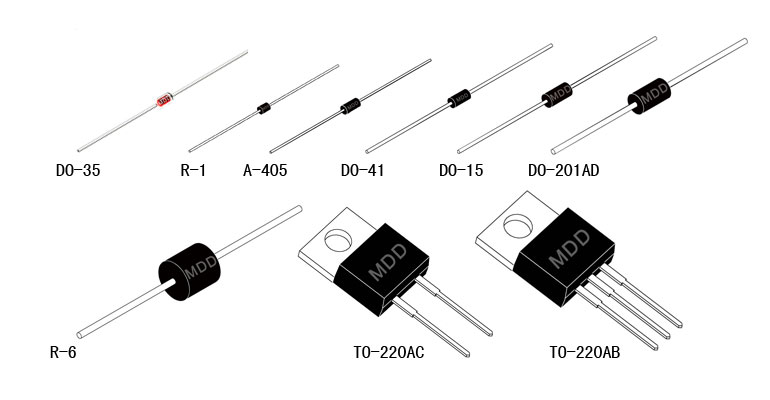
\includegraphics[width=.9\textwidth]{images/empaquetados_diodos.jpg}
      \caption{Diferentes empaquetados de diodos.}
    \end{figure}

    Para la identificacion de pines, utilizamos dos diodos 1N4007 y dos diodos 1N60, en empaquetados DO-15 y DO-35
    respectivamente.

    \begin{figure}[!ht]
      \centering
      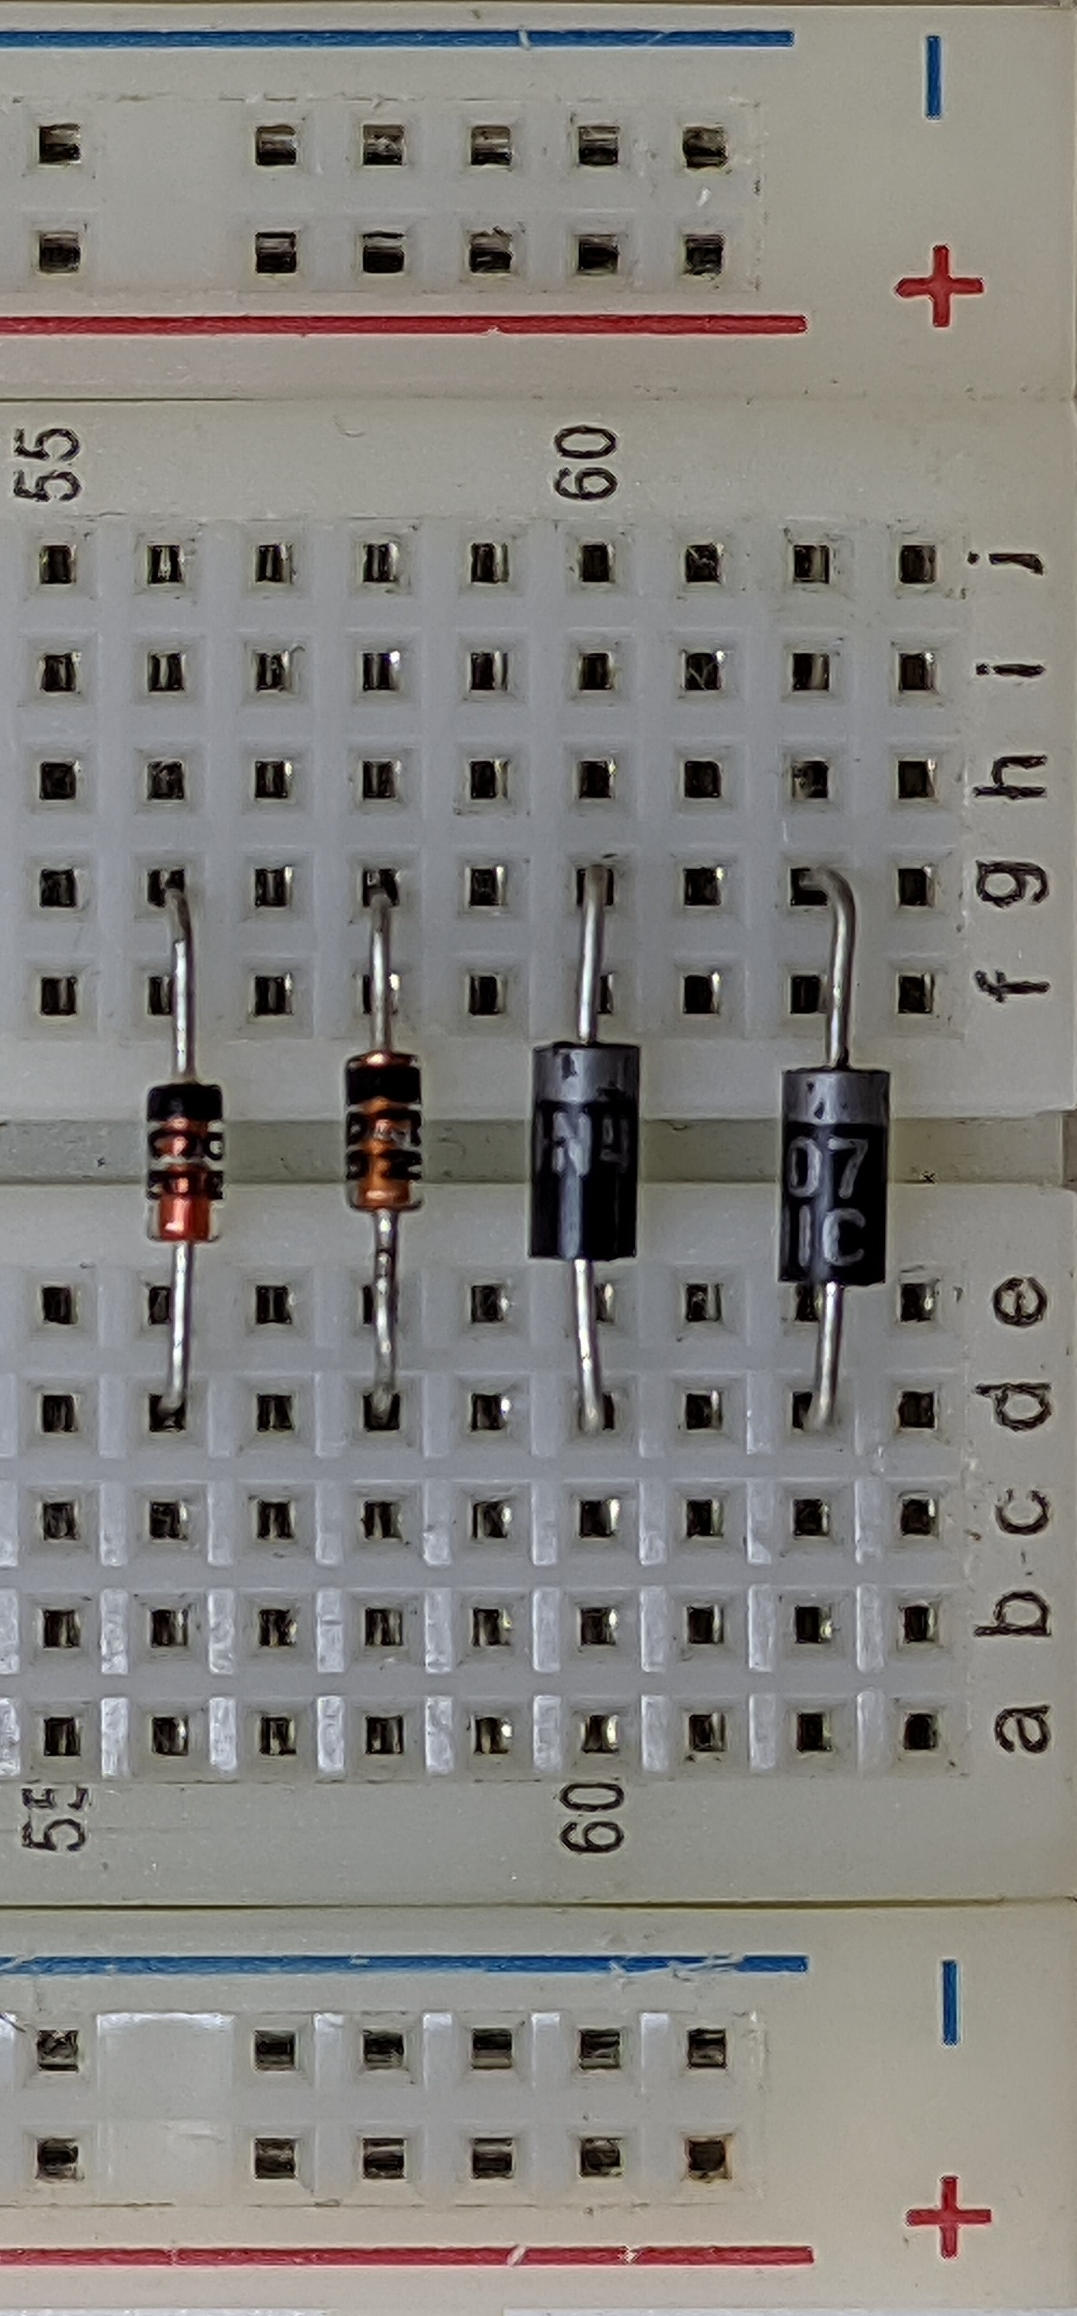
\includegraphics[angle=-90, width=.5\textwidth]{pictures/prot_diod-all.jpg}
      \caption{Diodos 1N60 (superior) y 1N4007 (inferior).}
    \end{figure}

    Se sabe que el diodo permite el paso de la corriente solo en un sentido. Si con el multimetro probamos las unicas
    dos posibilidades de circulacion de corriente, podremos identificar cual es el anodo y cual es el catodo:
    \begin{figure}[!ht]
      \begin{subfigure}[b]{1\textwidth}
        \centering
        \caption{Diodos polarizados en directa y sus caidas.}
        \begin{minipage}[b]{0.24\textwidth}
          \centering
          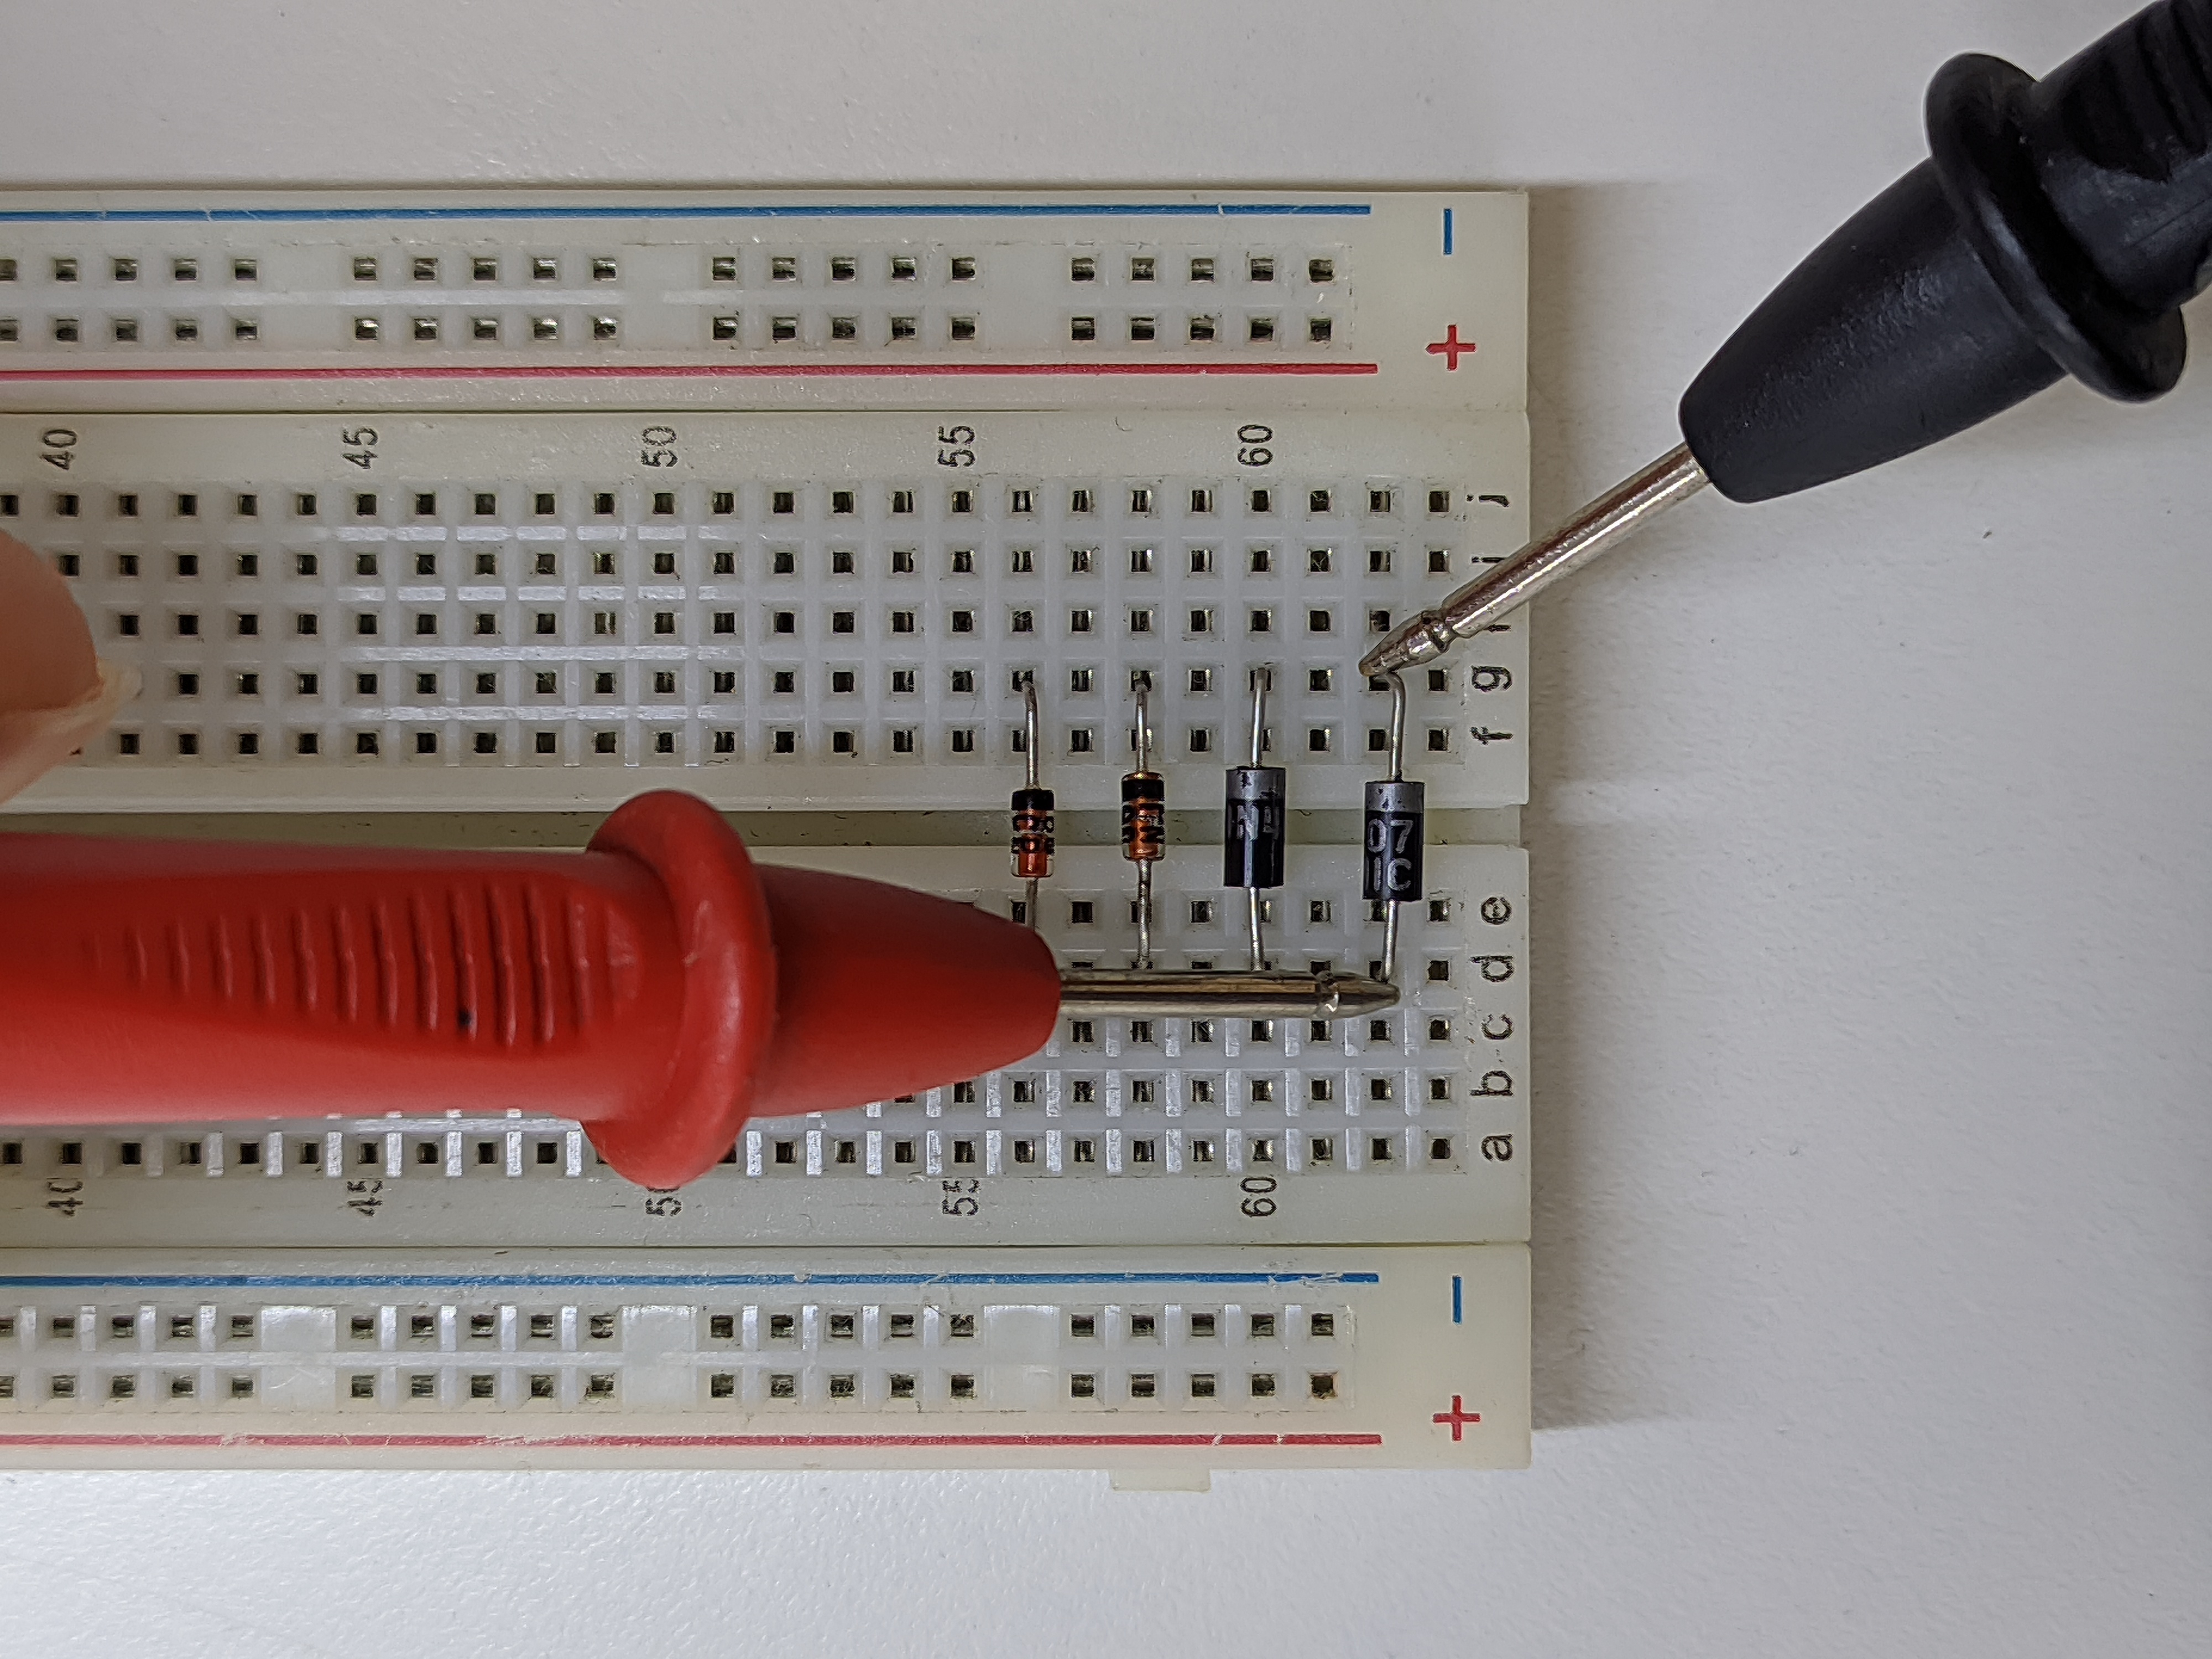
\includegraphics[angle=-90, width=1\textwidth]{pictures/prot_diod-1d.jpg}
          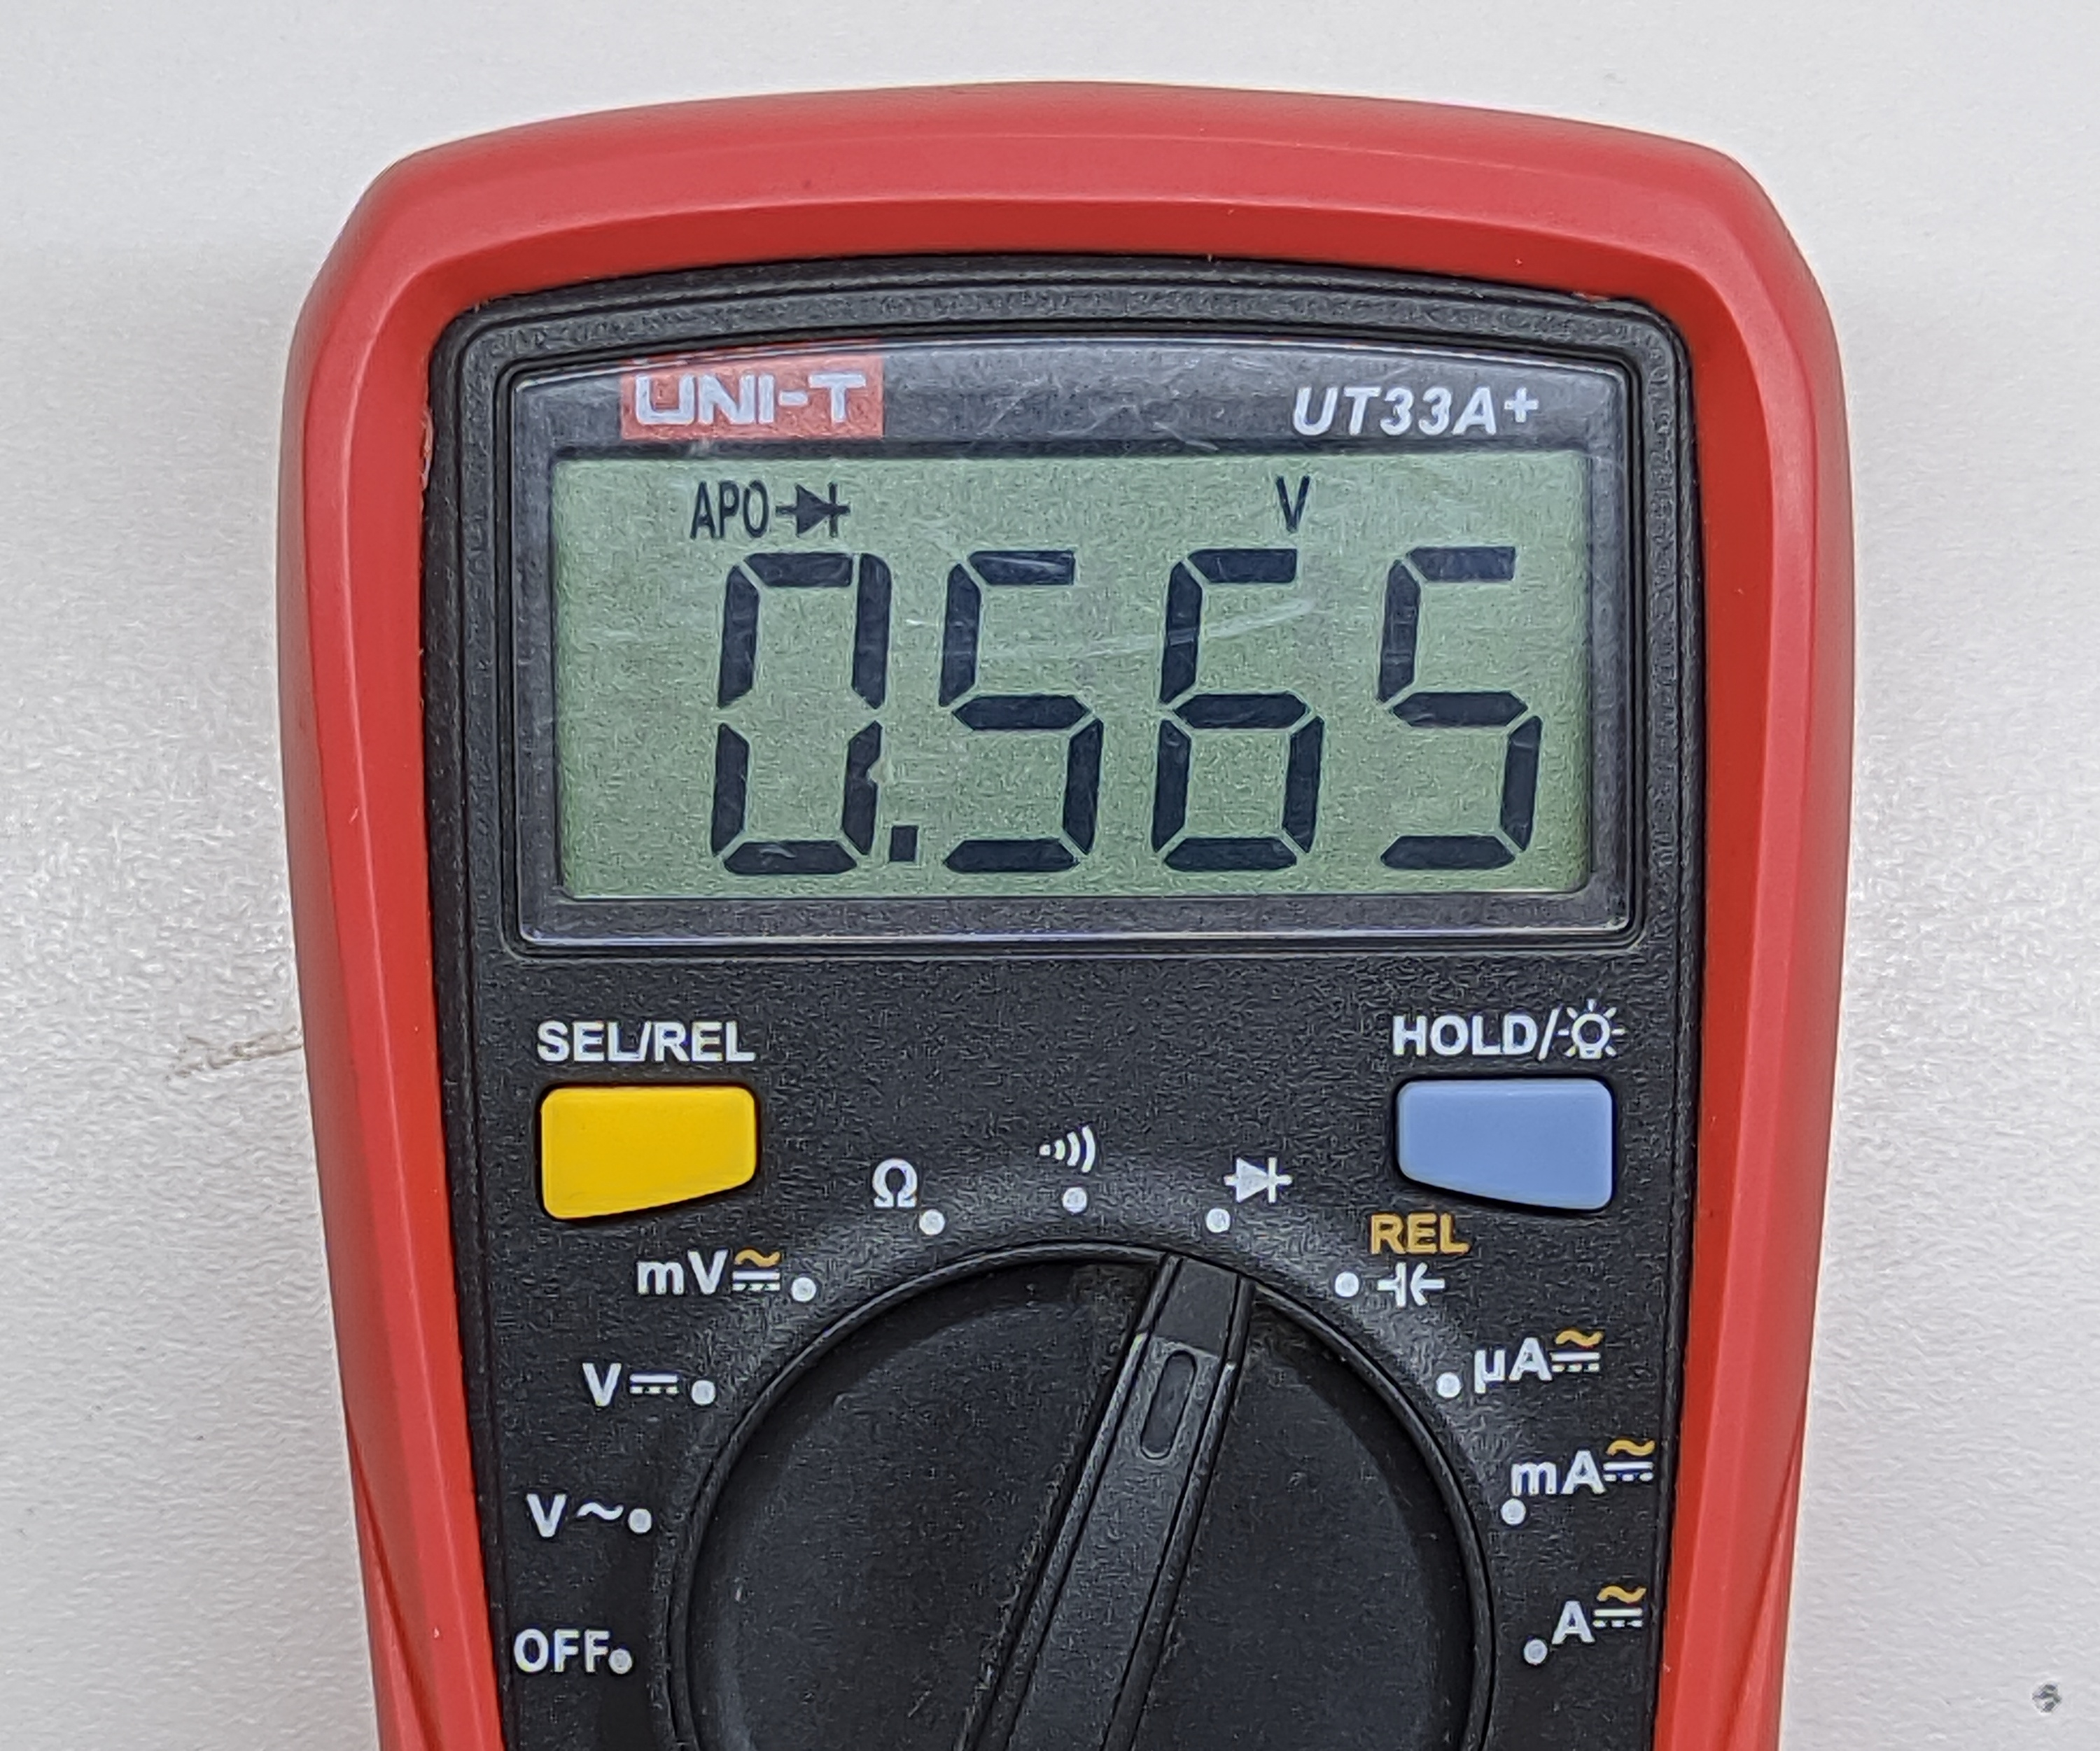
\includegraphics[width=1\textwidth]{pictures/mult_diod-1d.jpg}
        \end{minipage}
        \begin{minipage}[b]{0.24\textwidth}
          \centering
          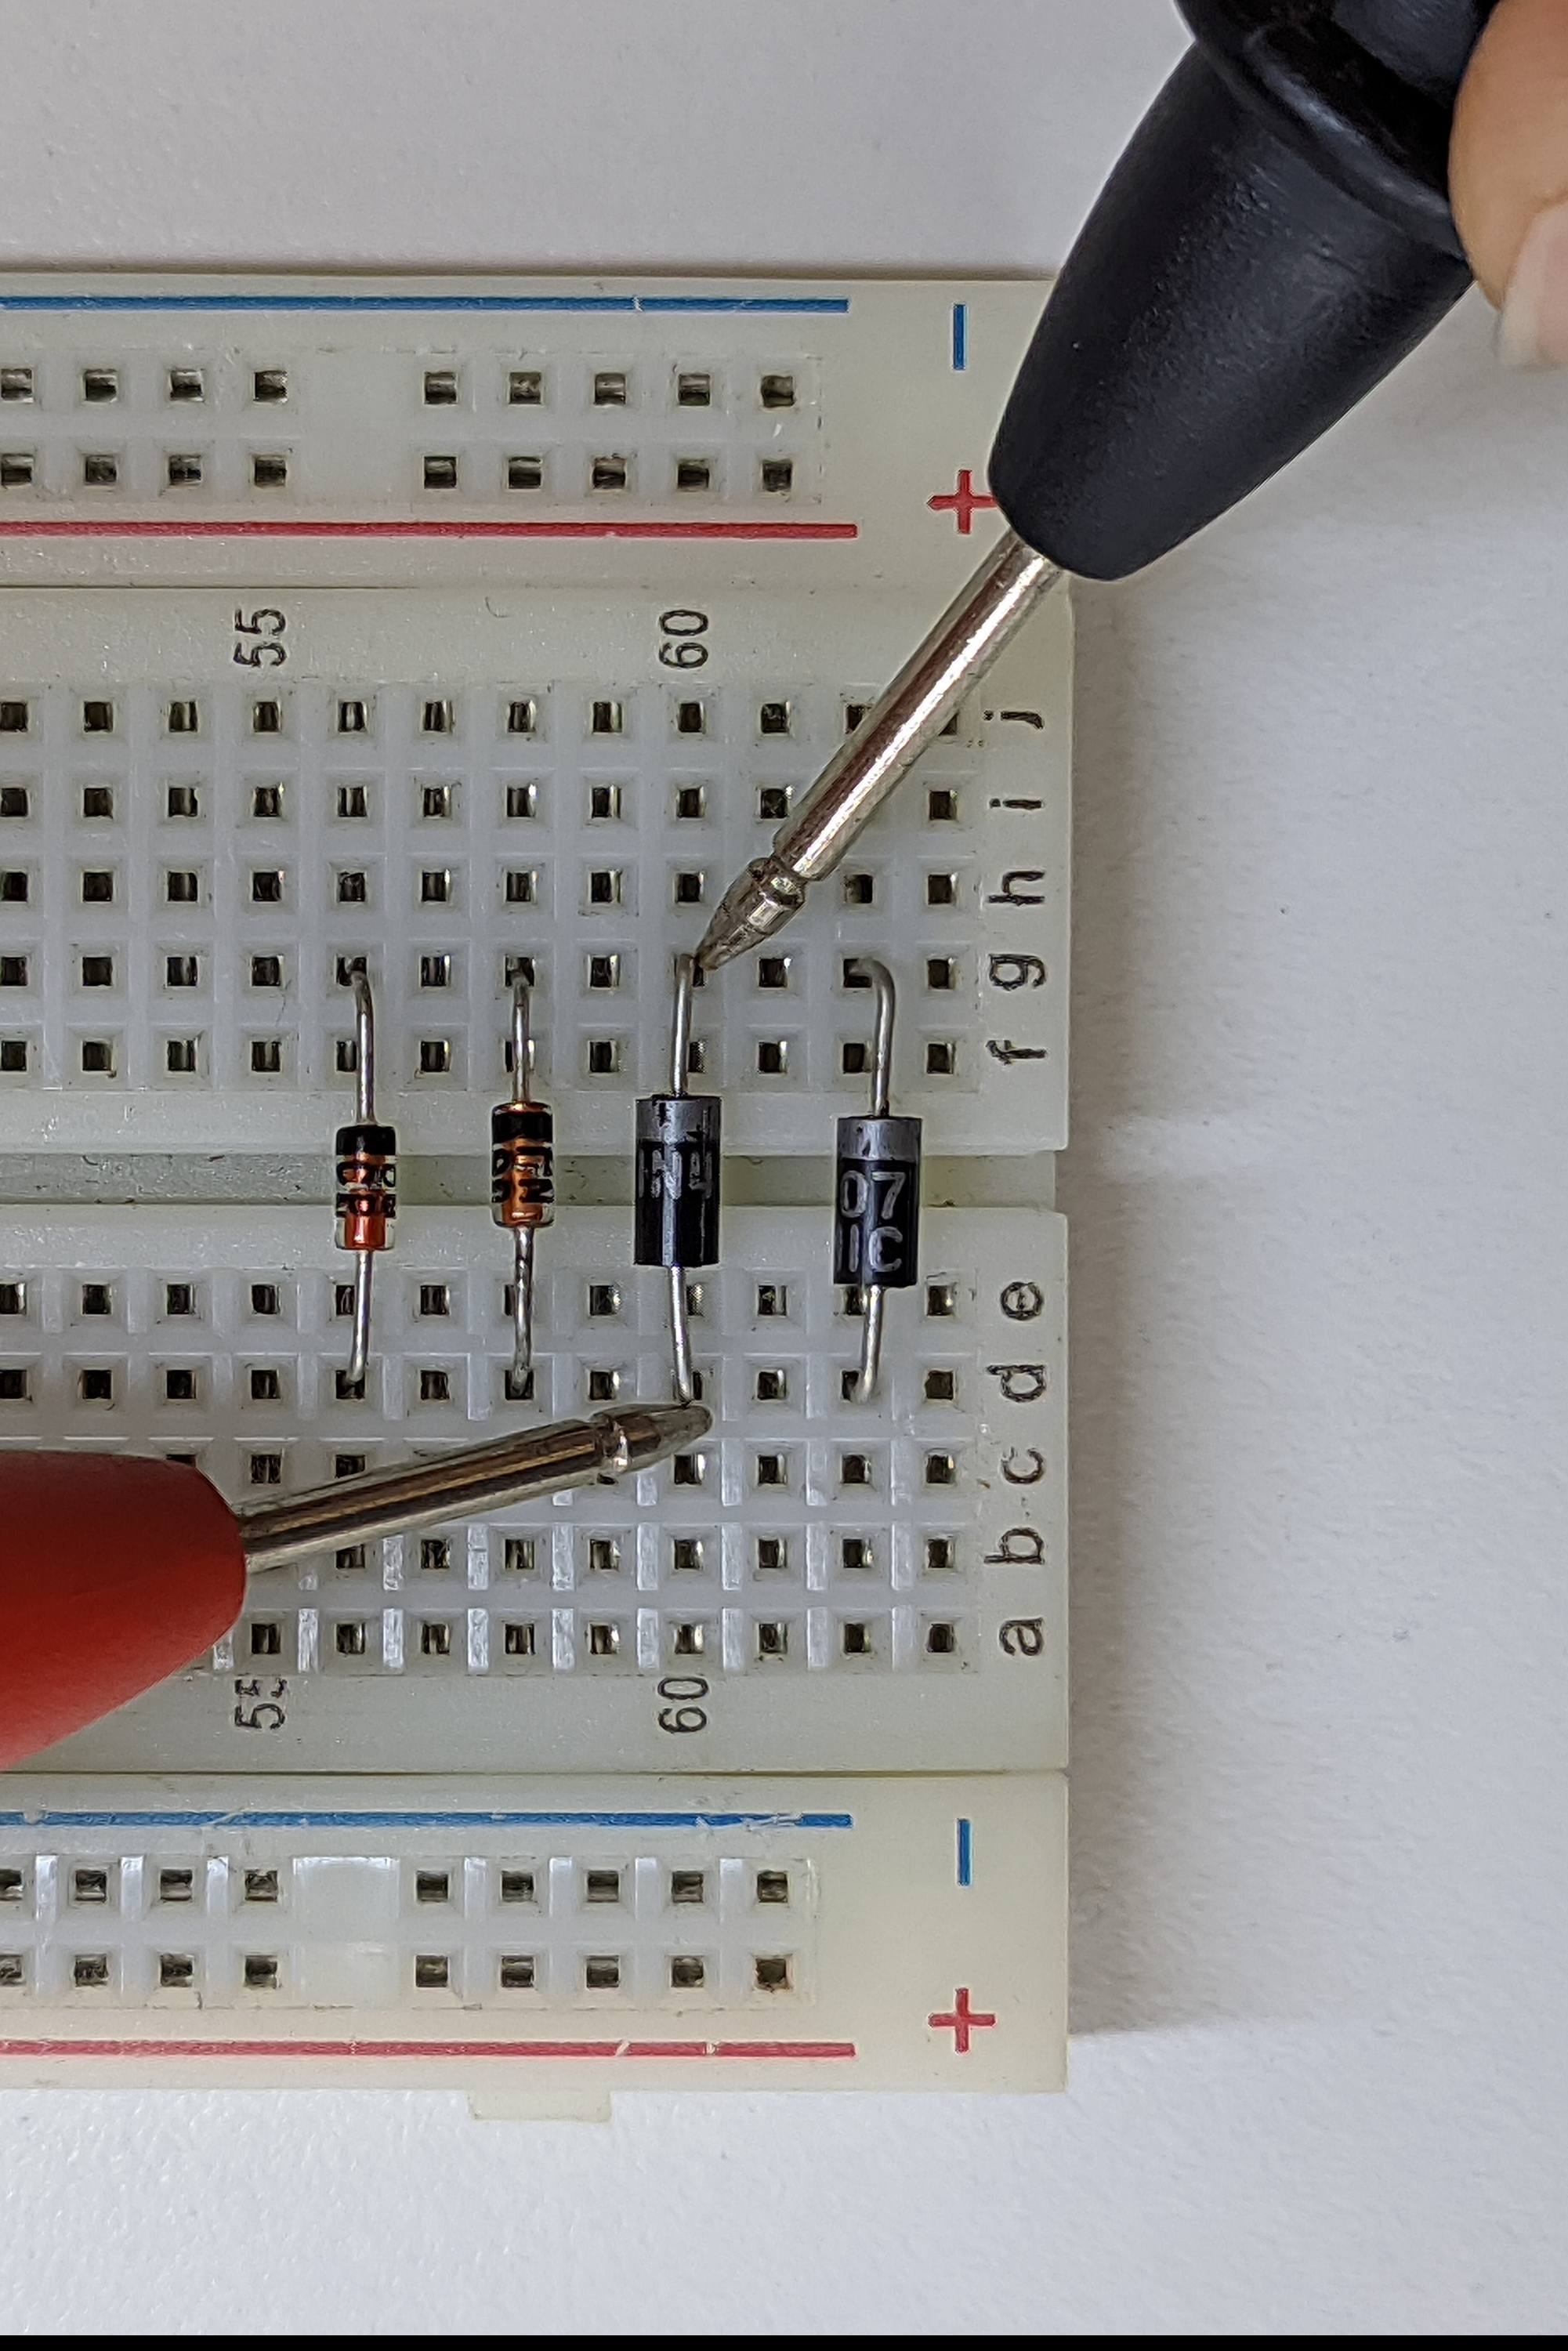
\includegraphics[angle=-90, width=1\textwidth]{pictures/prot_diod-2d.jpg}
          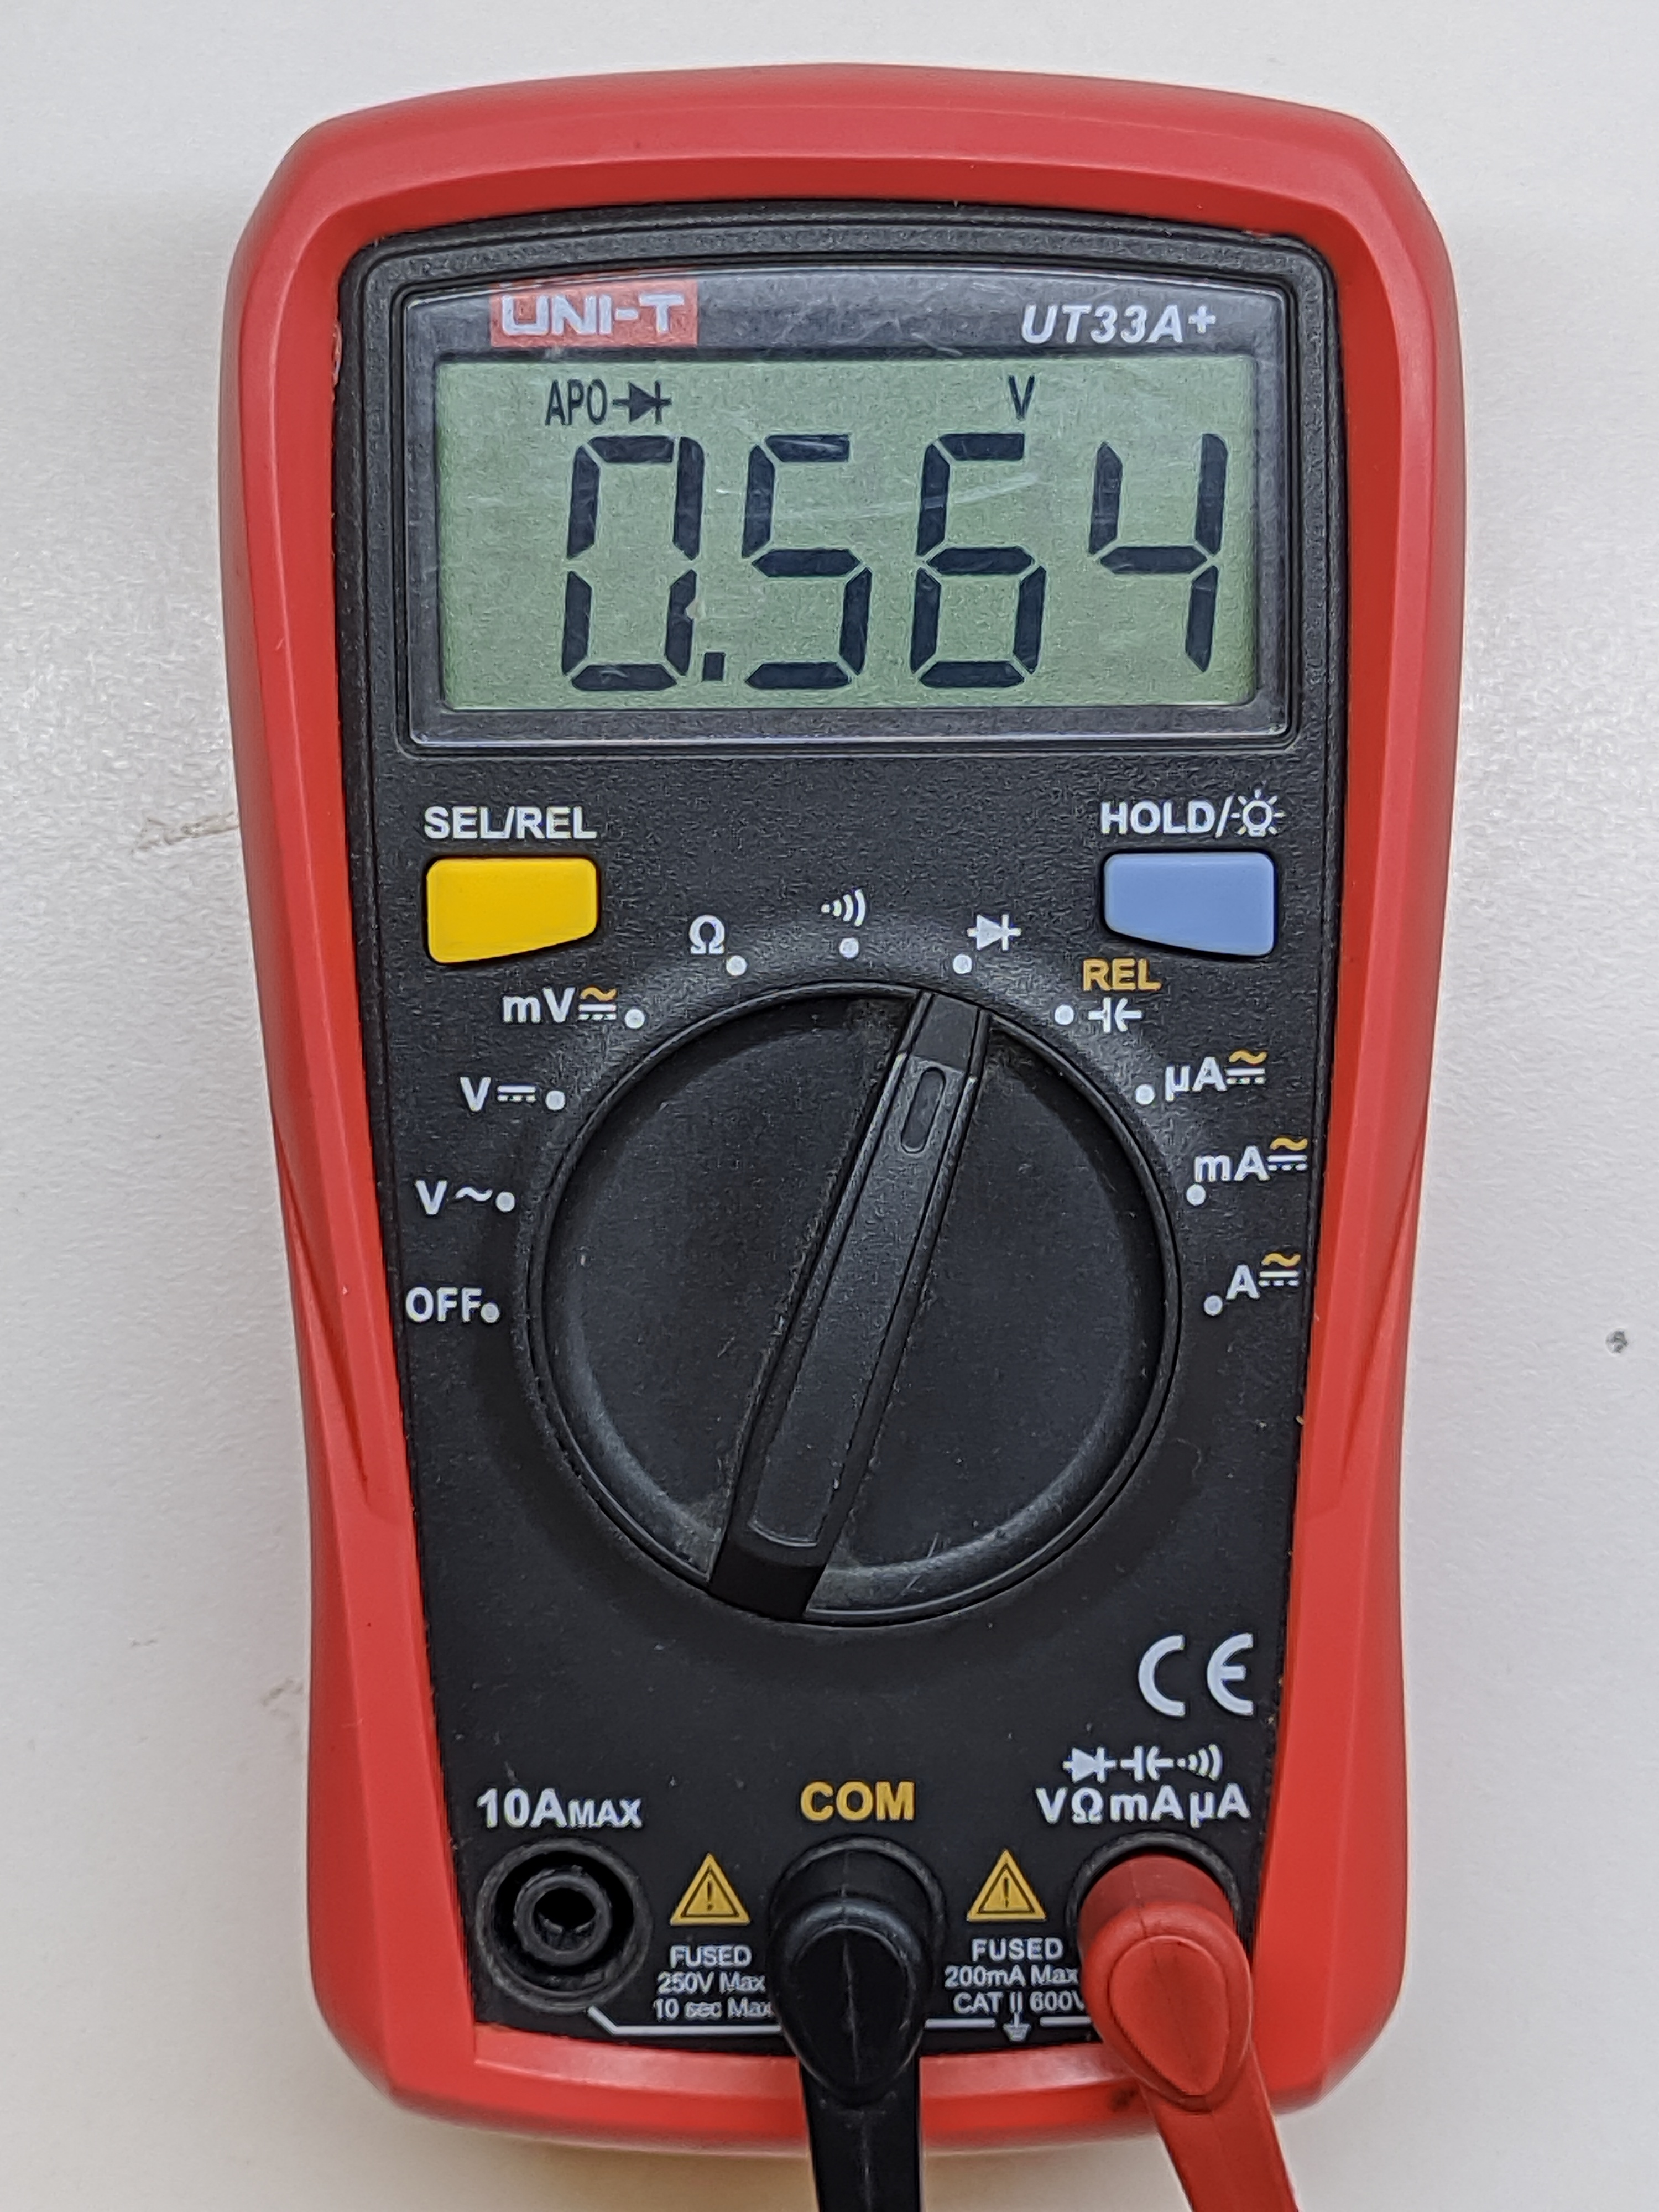
\includegraphics[width=1\textwidth]{pictures/mult_diod-2d.jpg}
        \end{minipage}
        \begin{minipage}[b]{0.24\textwidth}
          \centering
          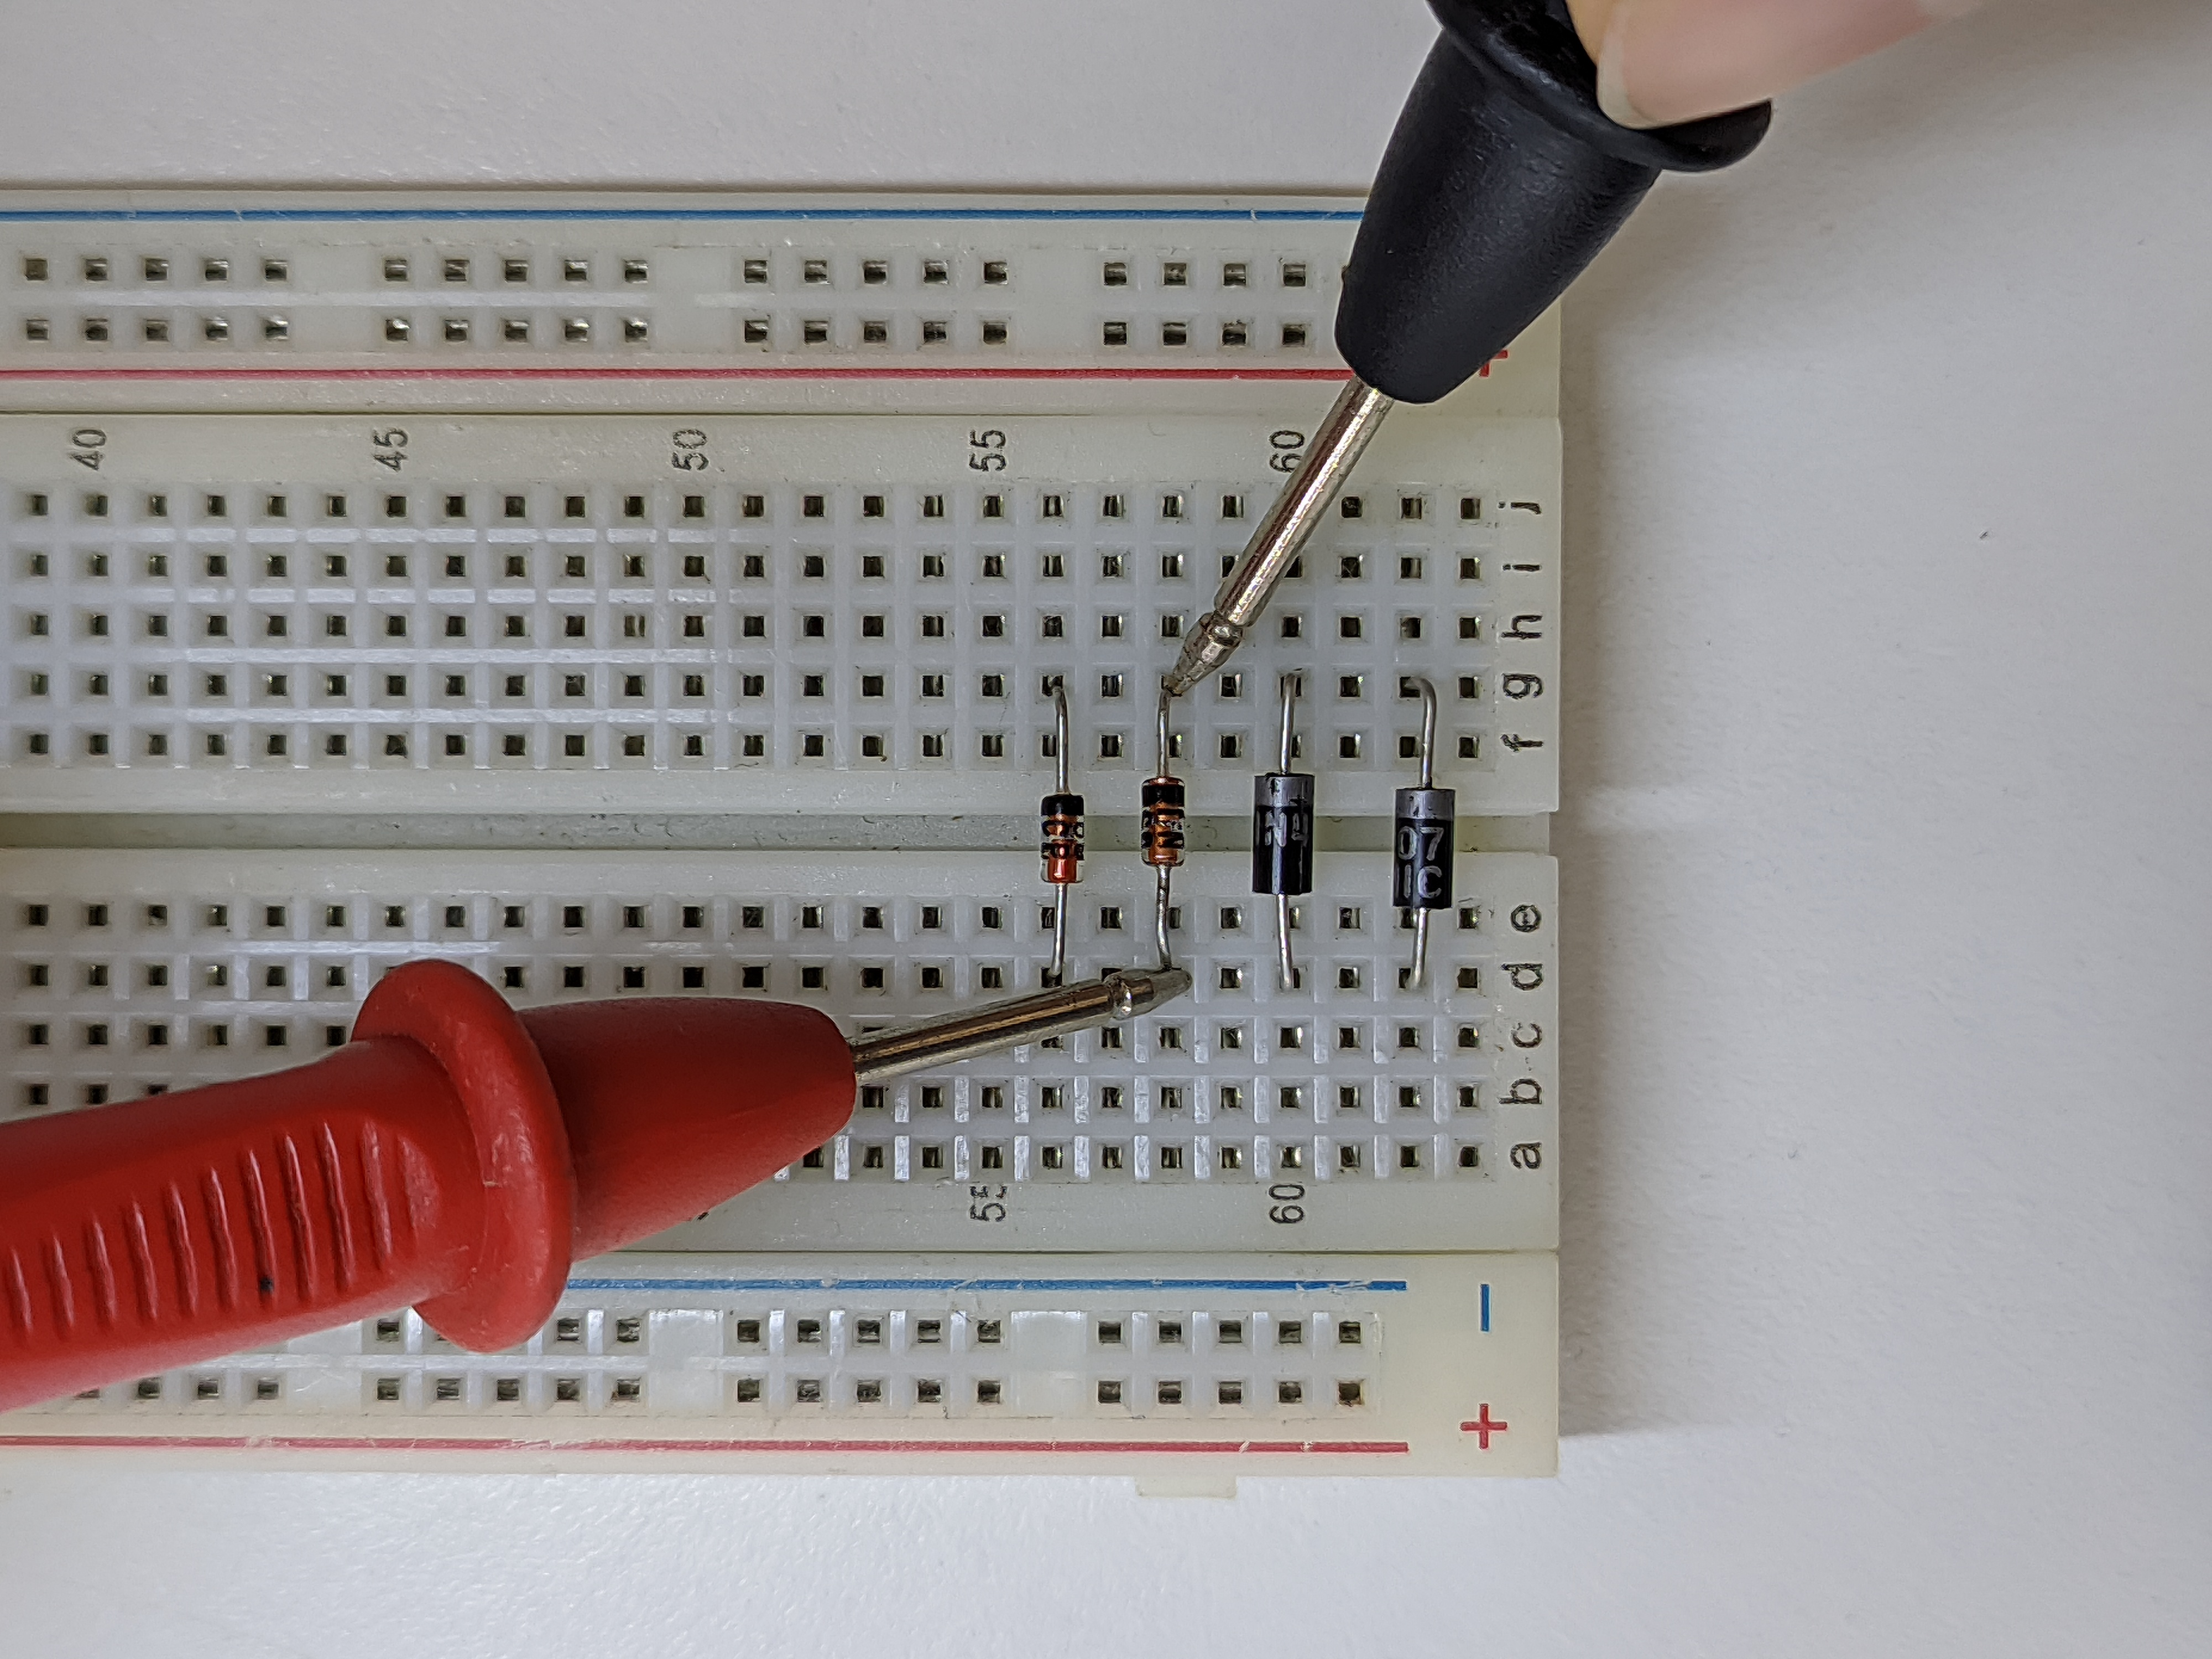
\includegraphics[angle=-90, width=1\textwidth]{pictures/prot_diod-3d.jpg}
          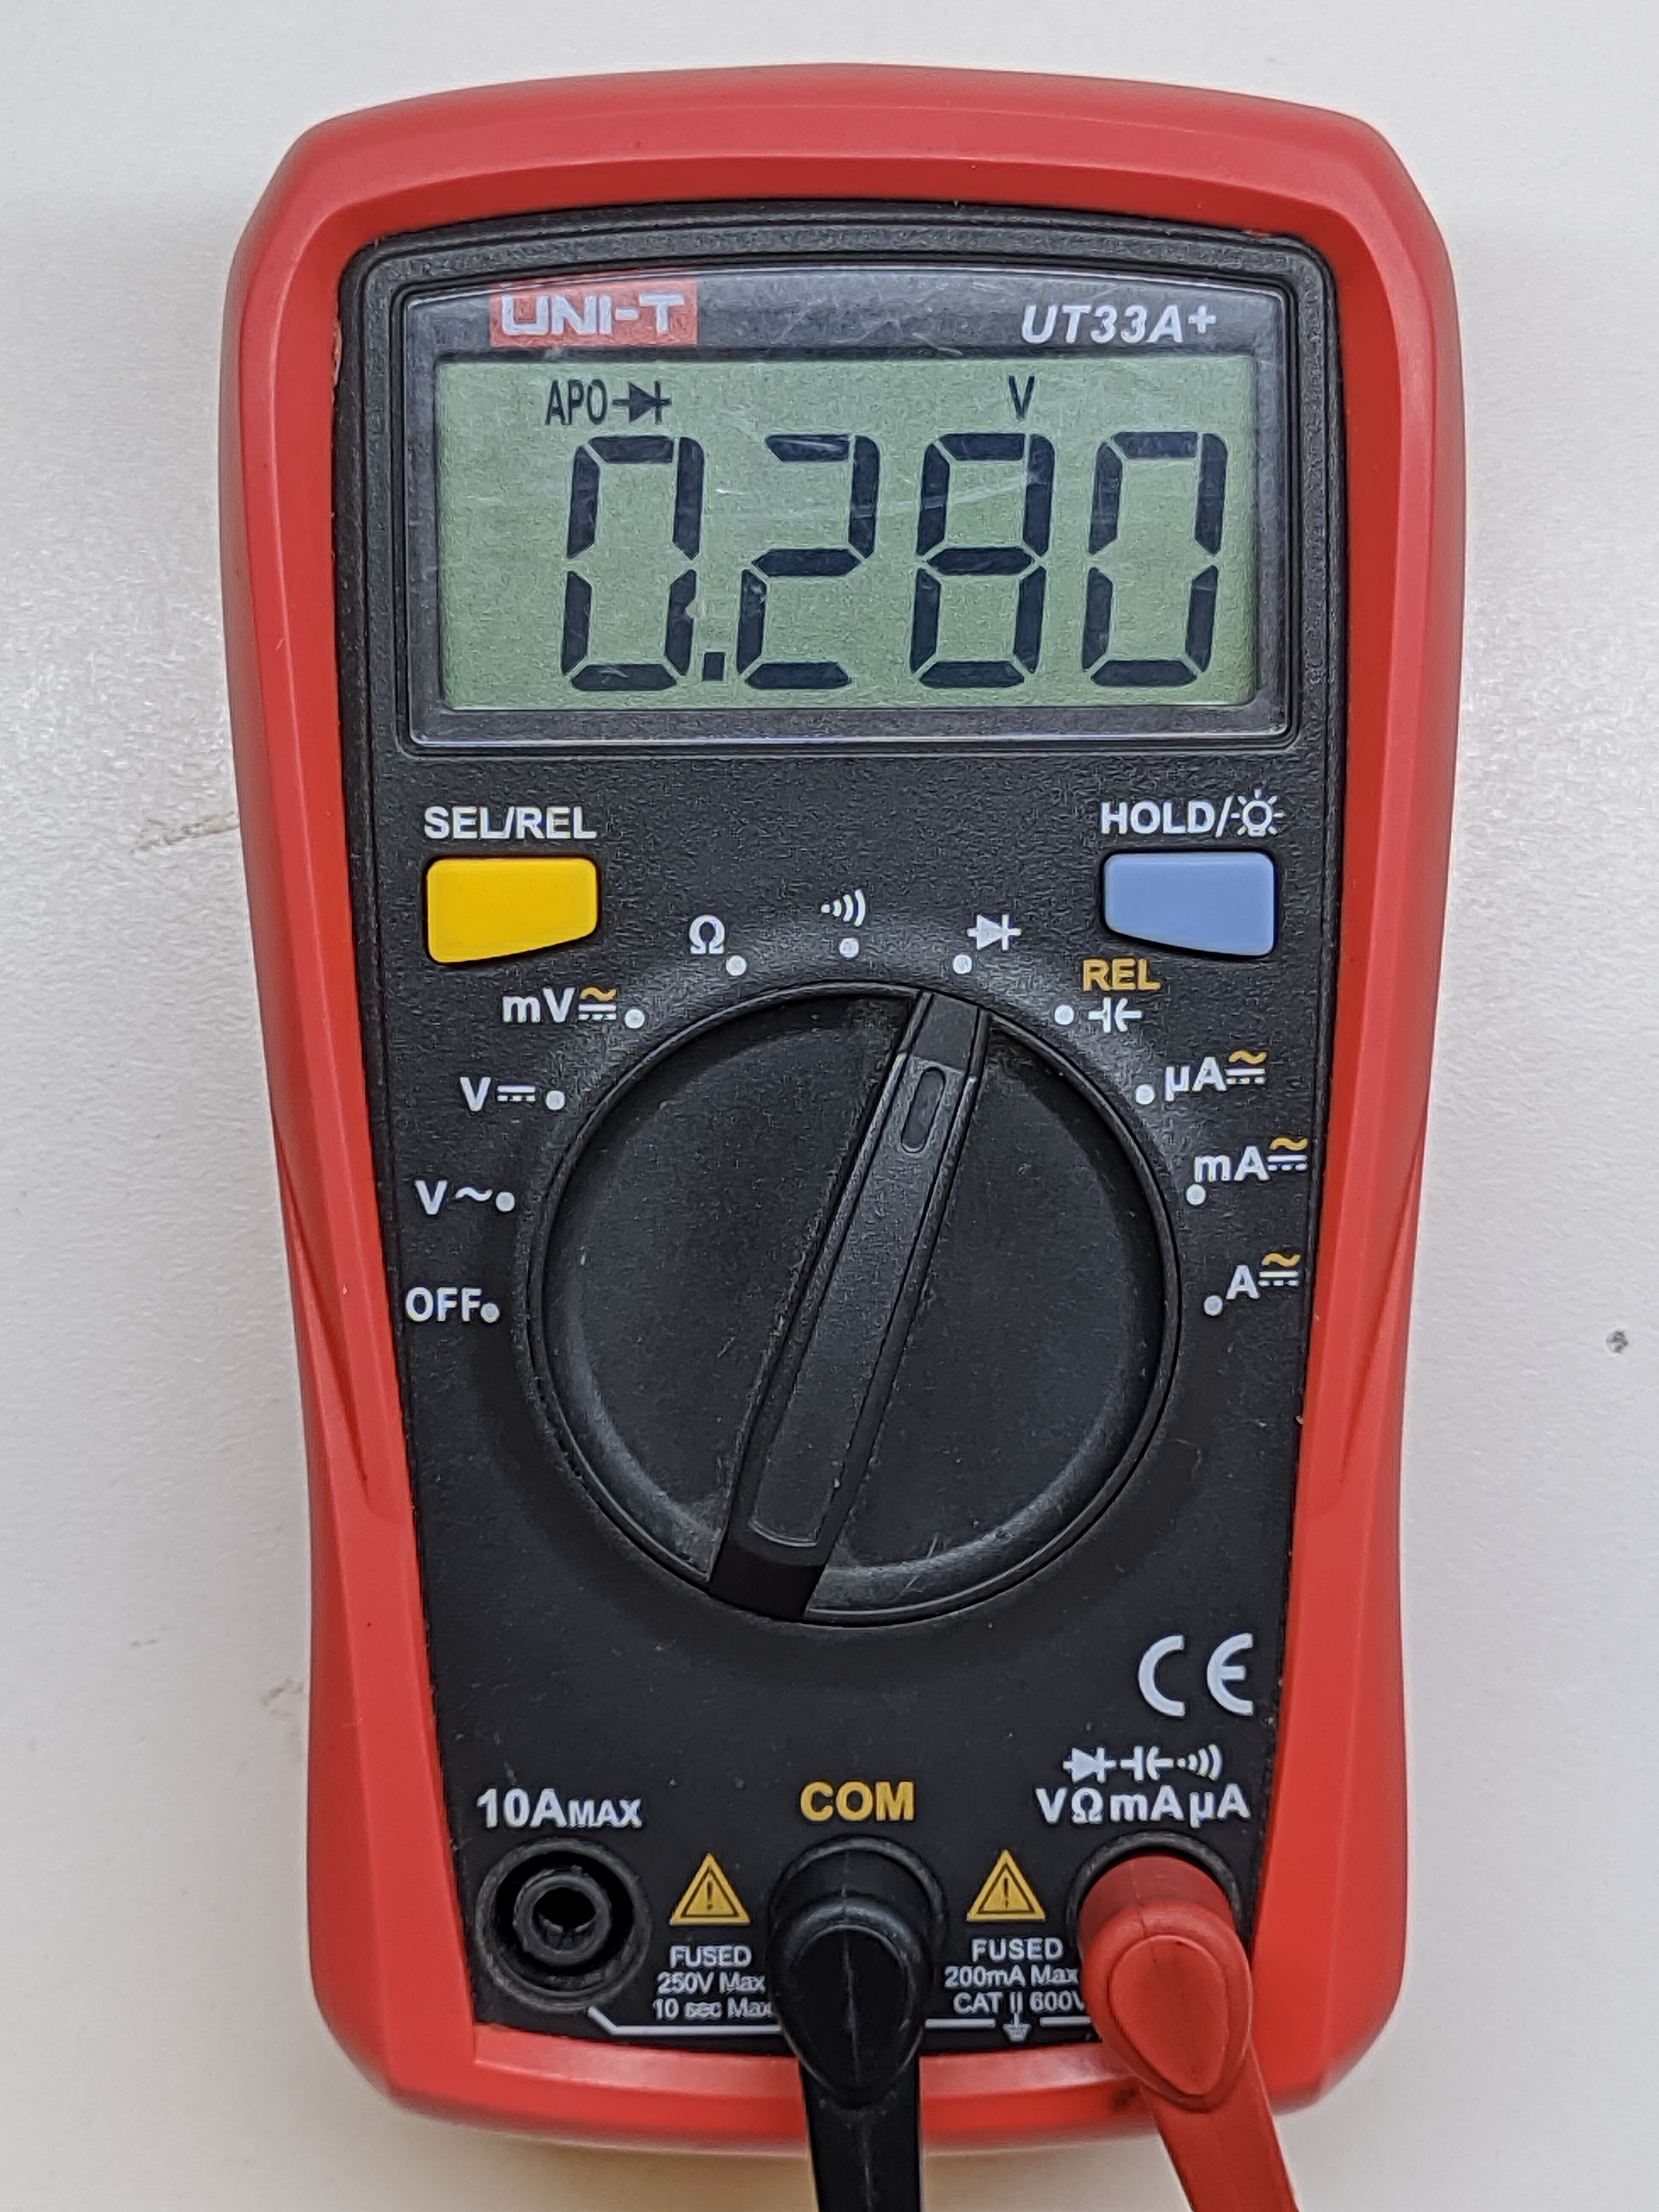
\includegraphics[width=1\textwidth]{pictures/mult_diod-3d.jpg}
        \end{minipage}
        \begin{minipage}[b]{0.24\textwidth}
          \centering
          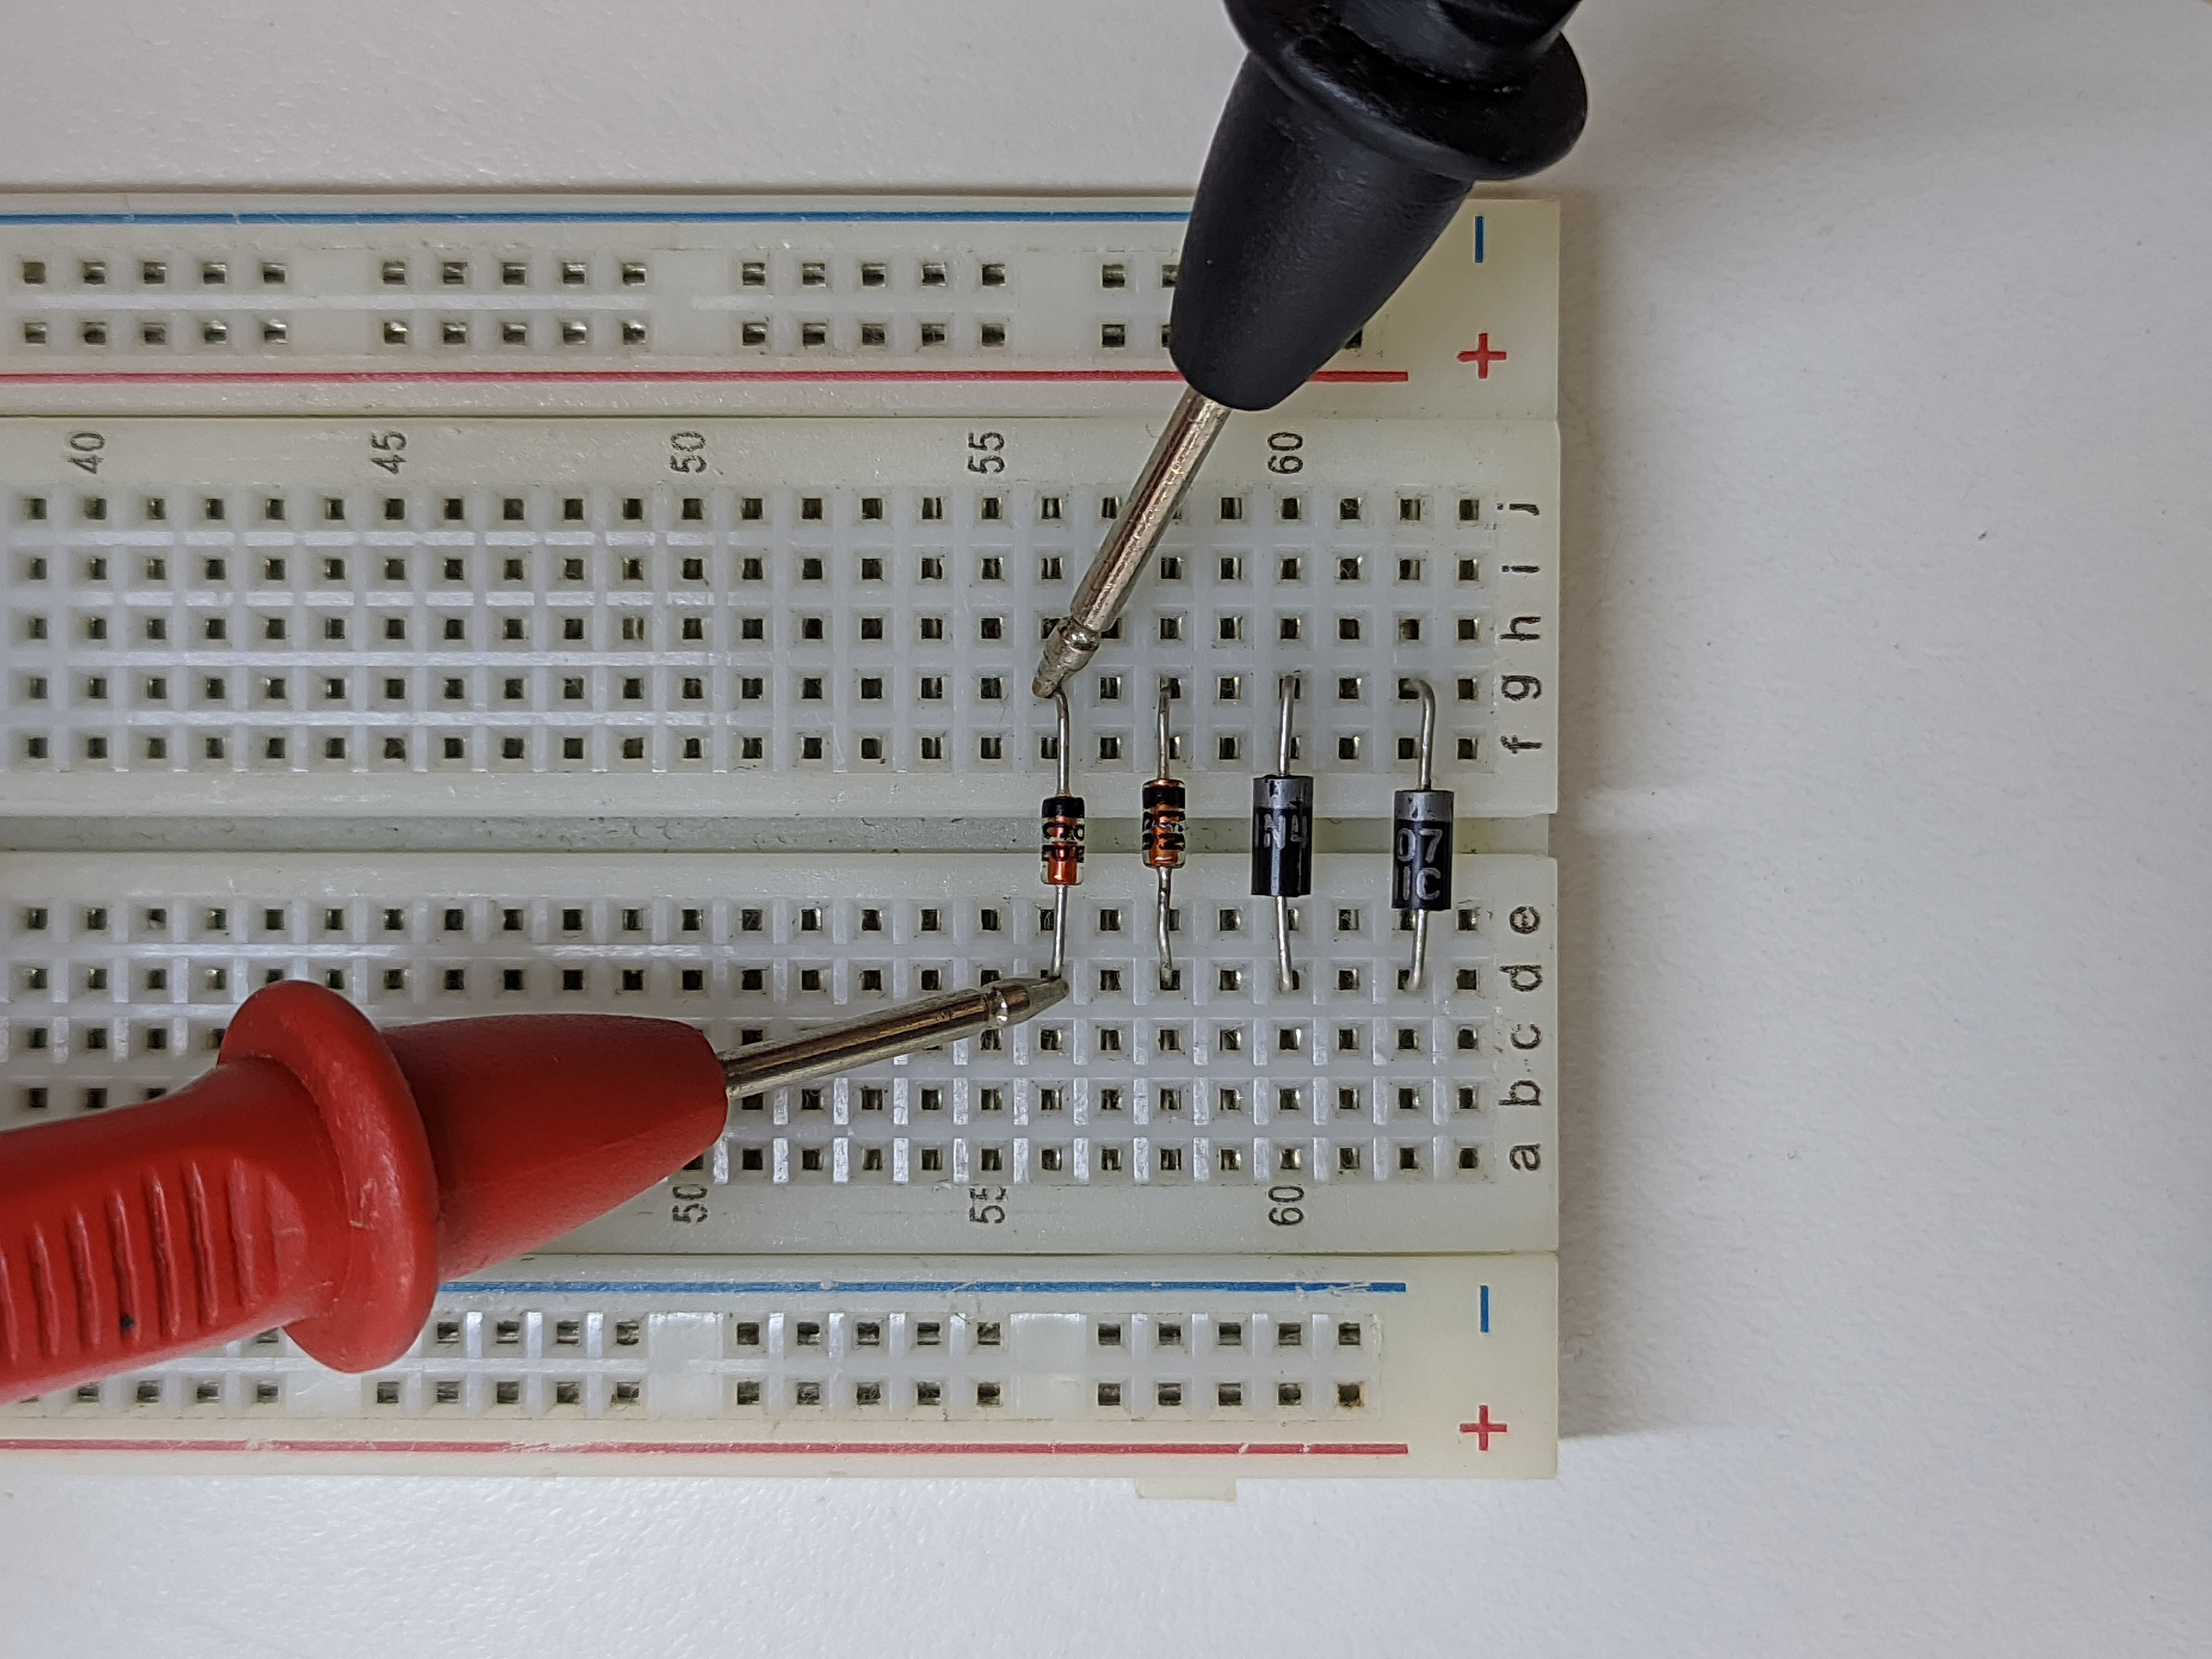
\includegraphics[angle=-90, width=1\textwidth]{pictures/prot_diod-4d.jpg}
          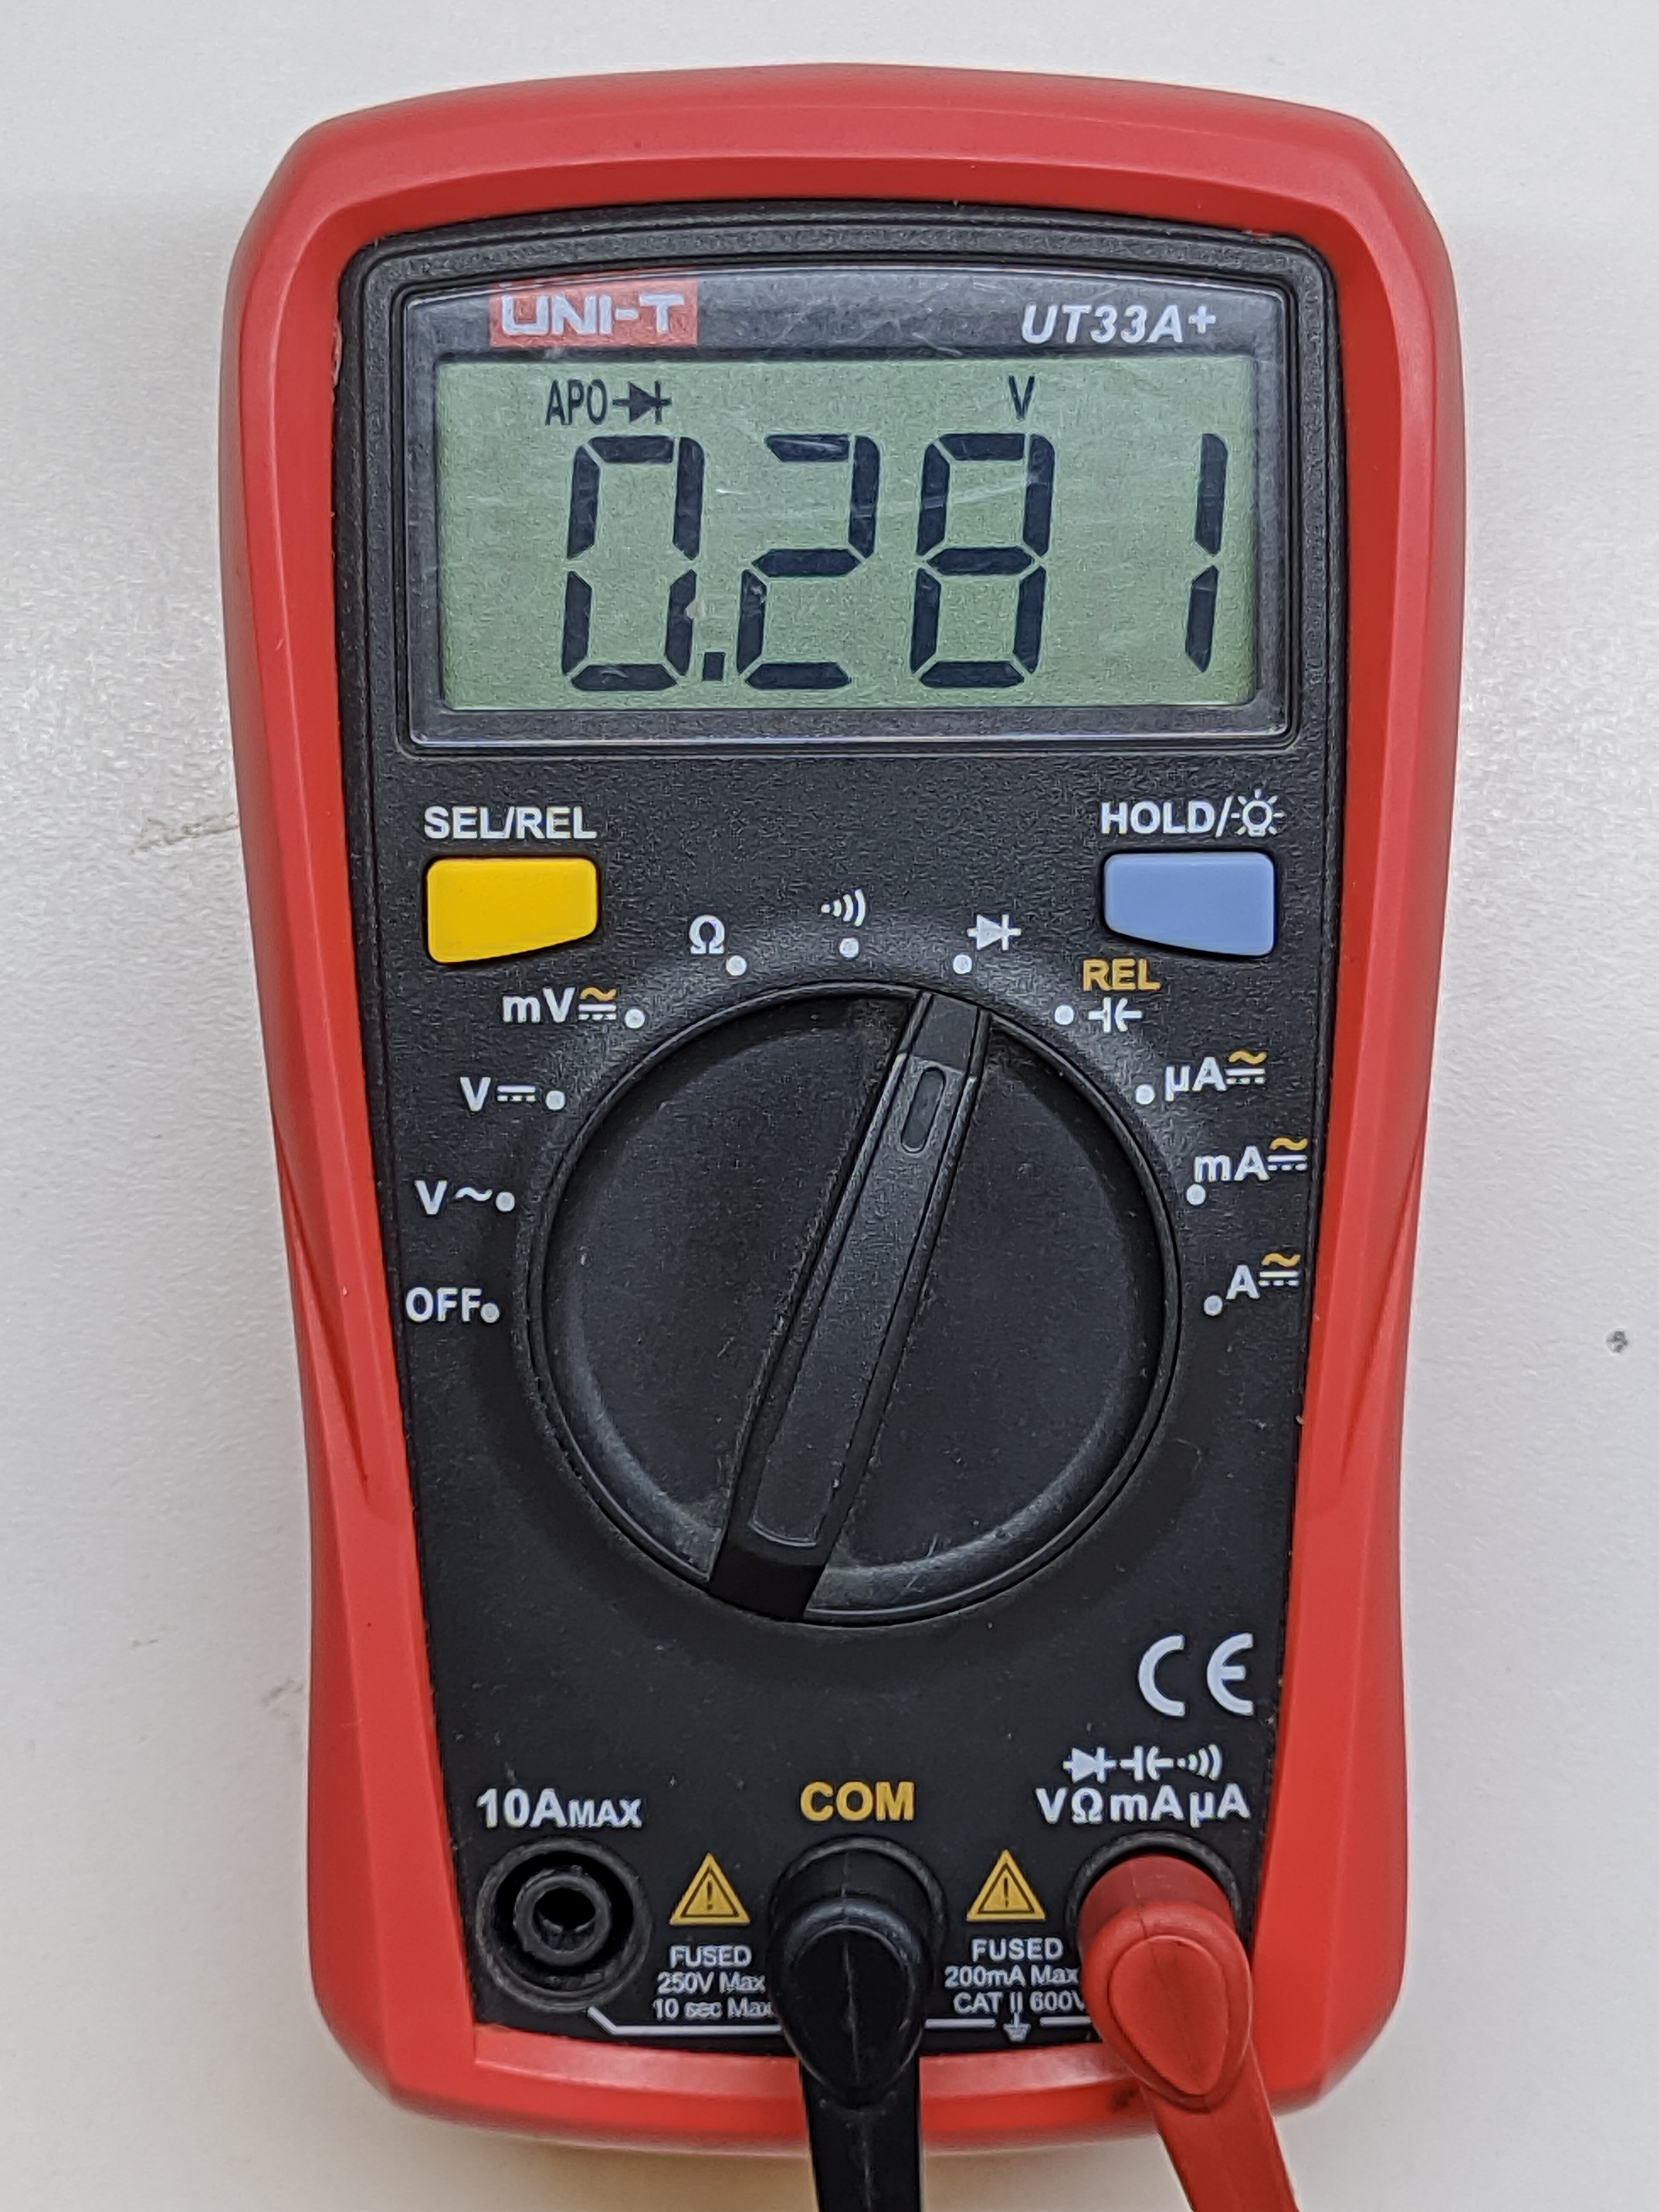
\includegraphics[width=1\textwidth]{pictures/mult_diod-4d.jpg}
        \end{minipage}
      \end{subfigure}
      \begin{subfigure}[b]{1\textwidth}
        \centering
        \caption{Diodos polarizados en inversa y sus caidas.}
        \begin{minipage}[b]{0.24\textwidth}
          \centering
          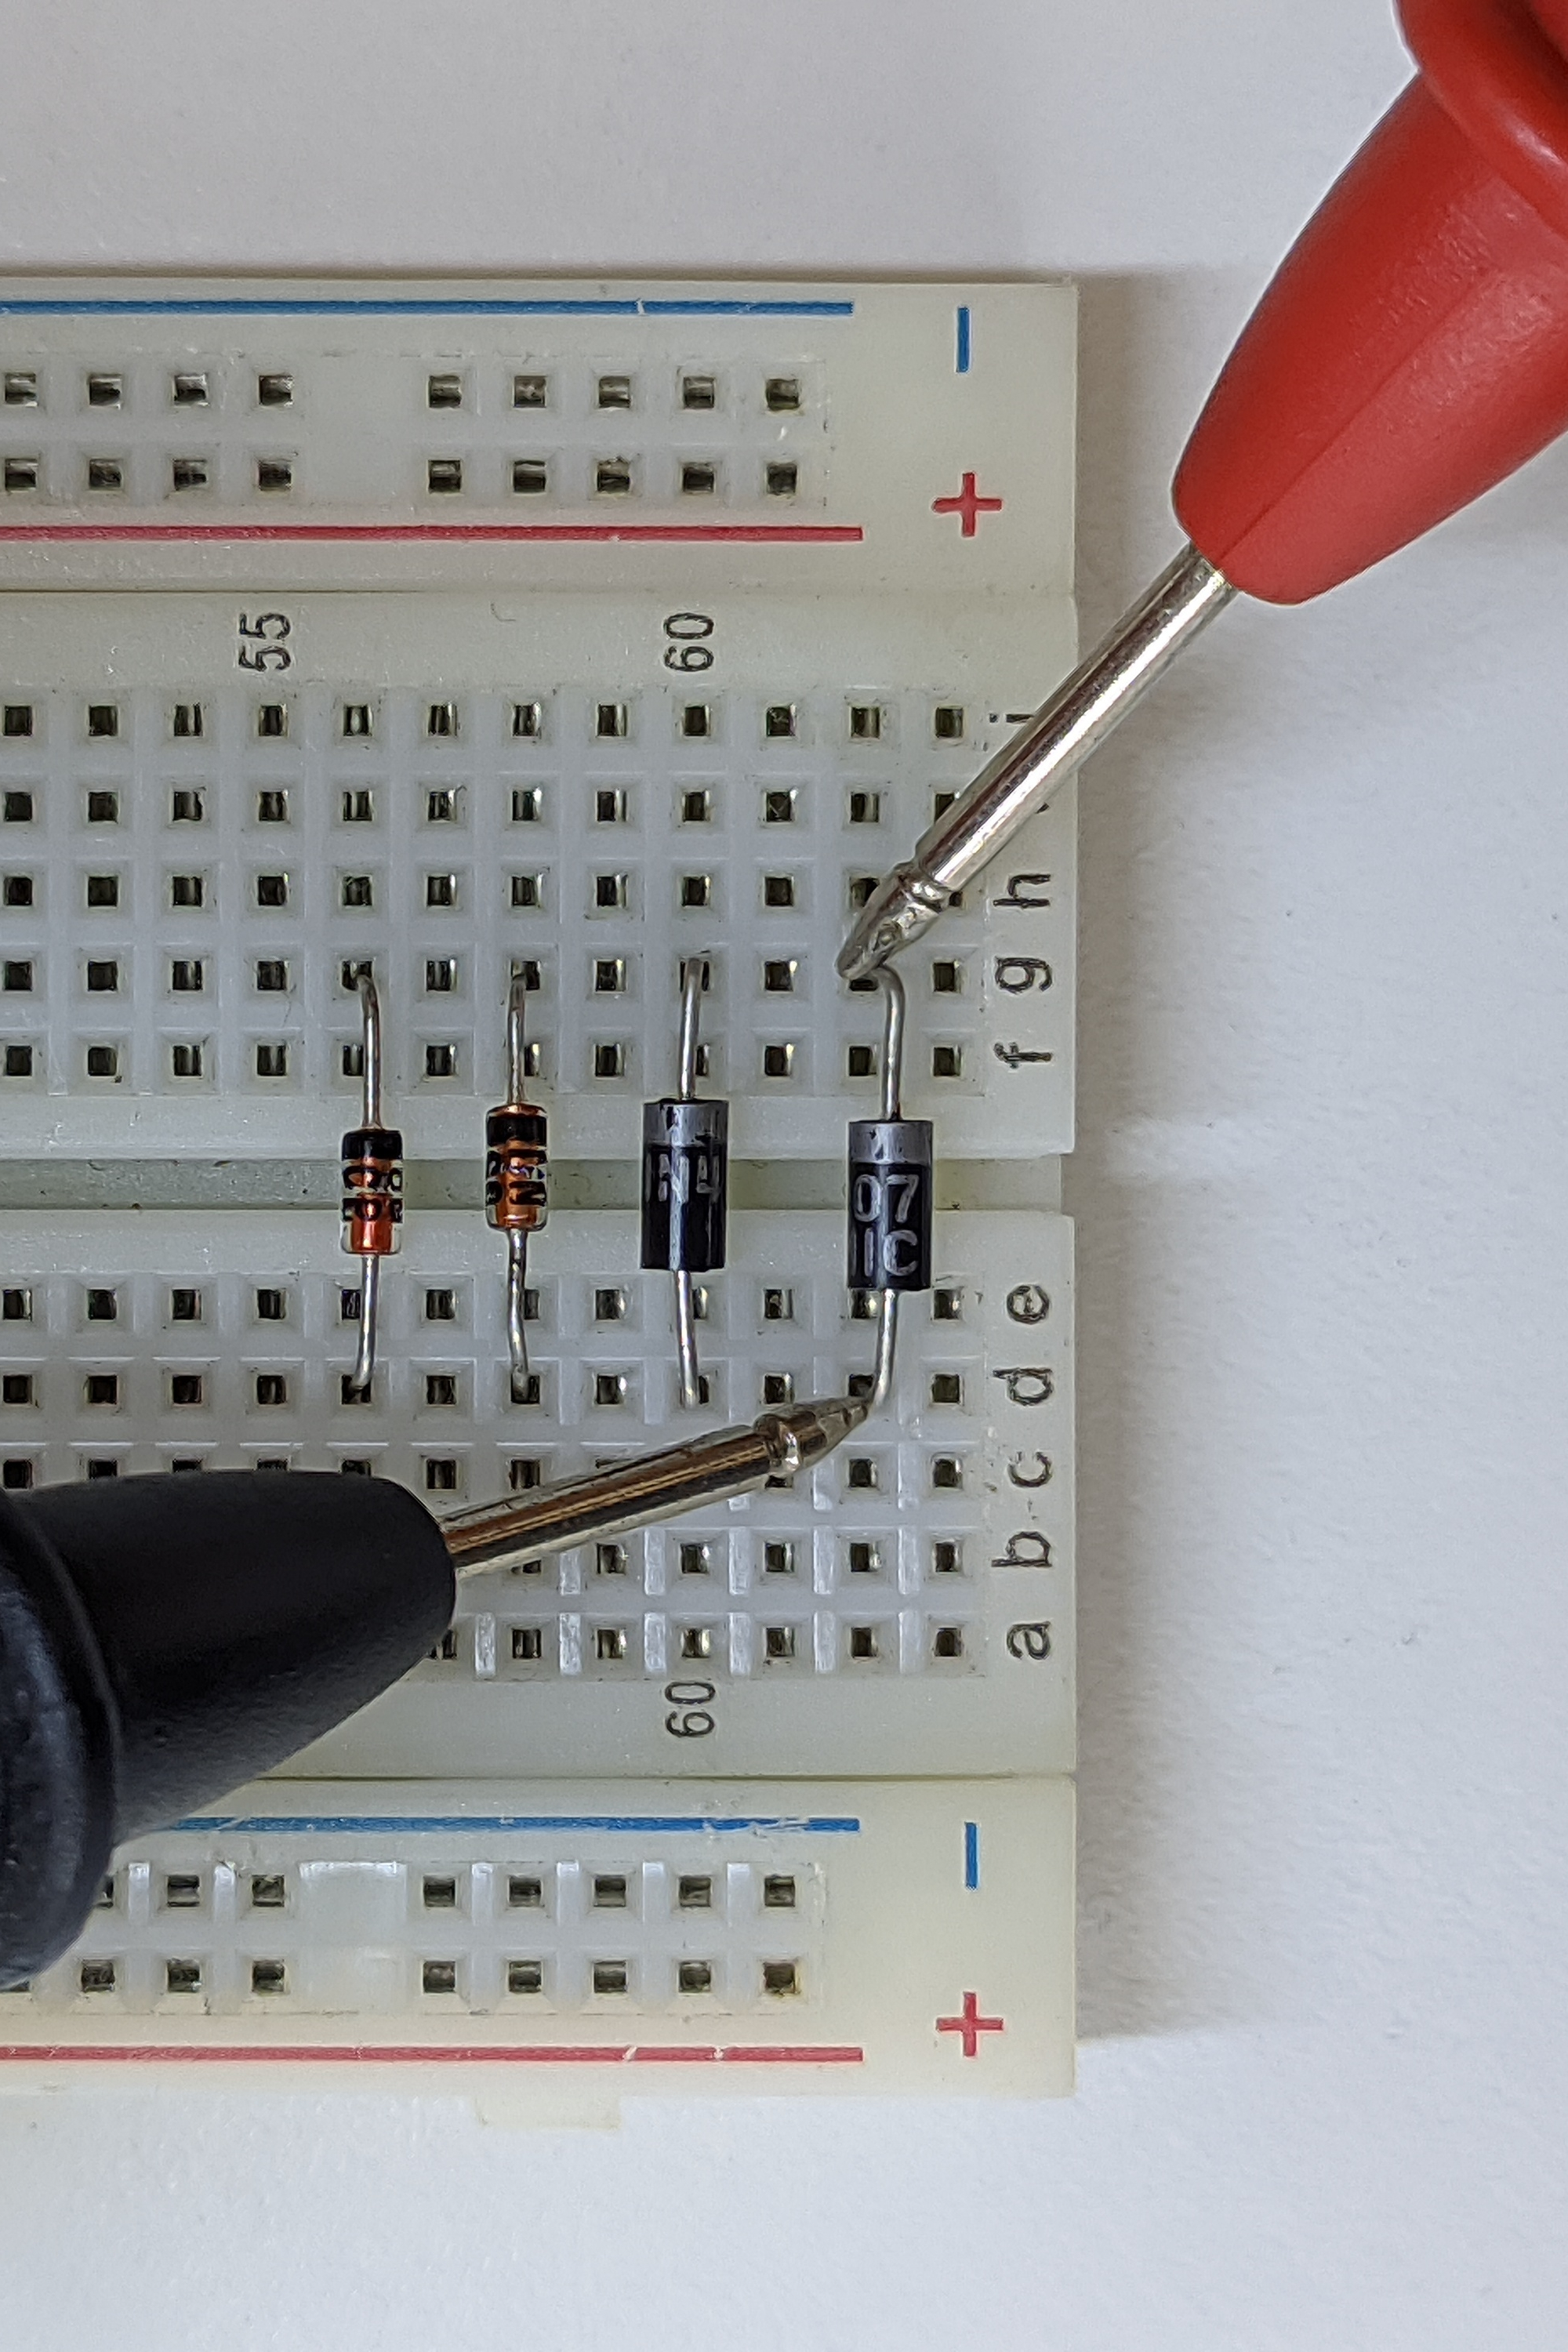
\includegraphics[angle=-90, width=1\textwidth]{pictures/prot_diod-1i.jpg}
          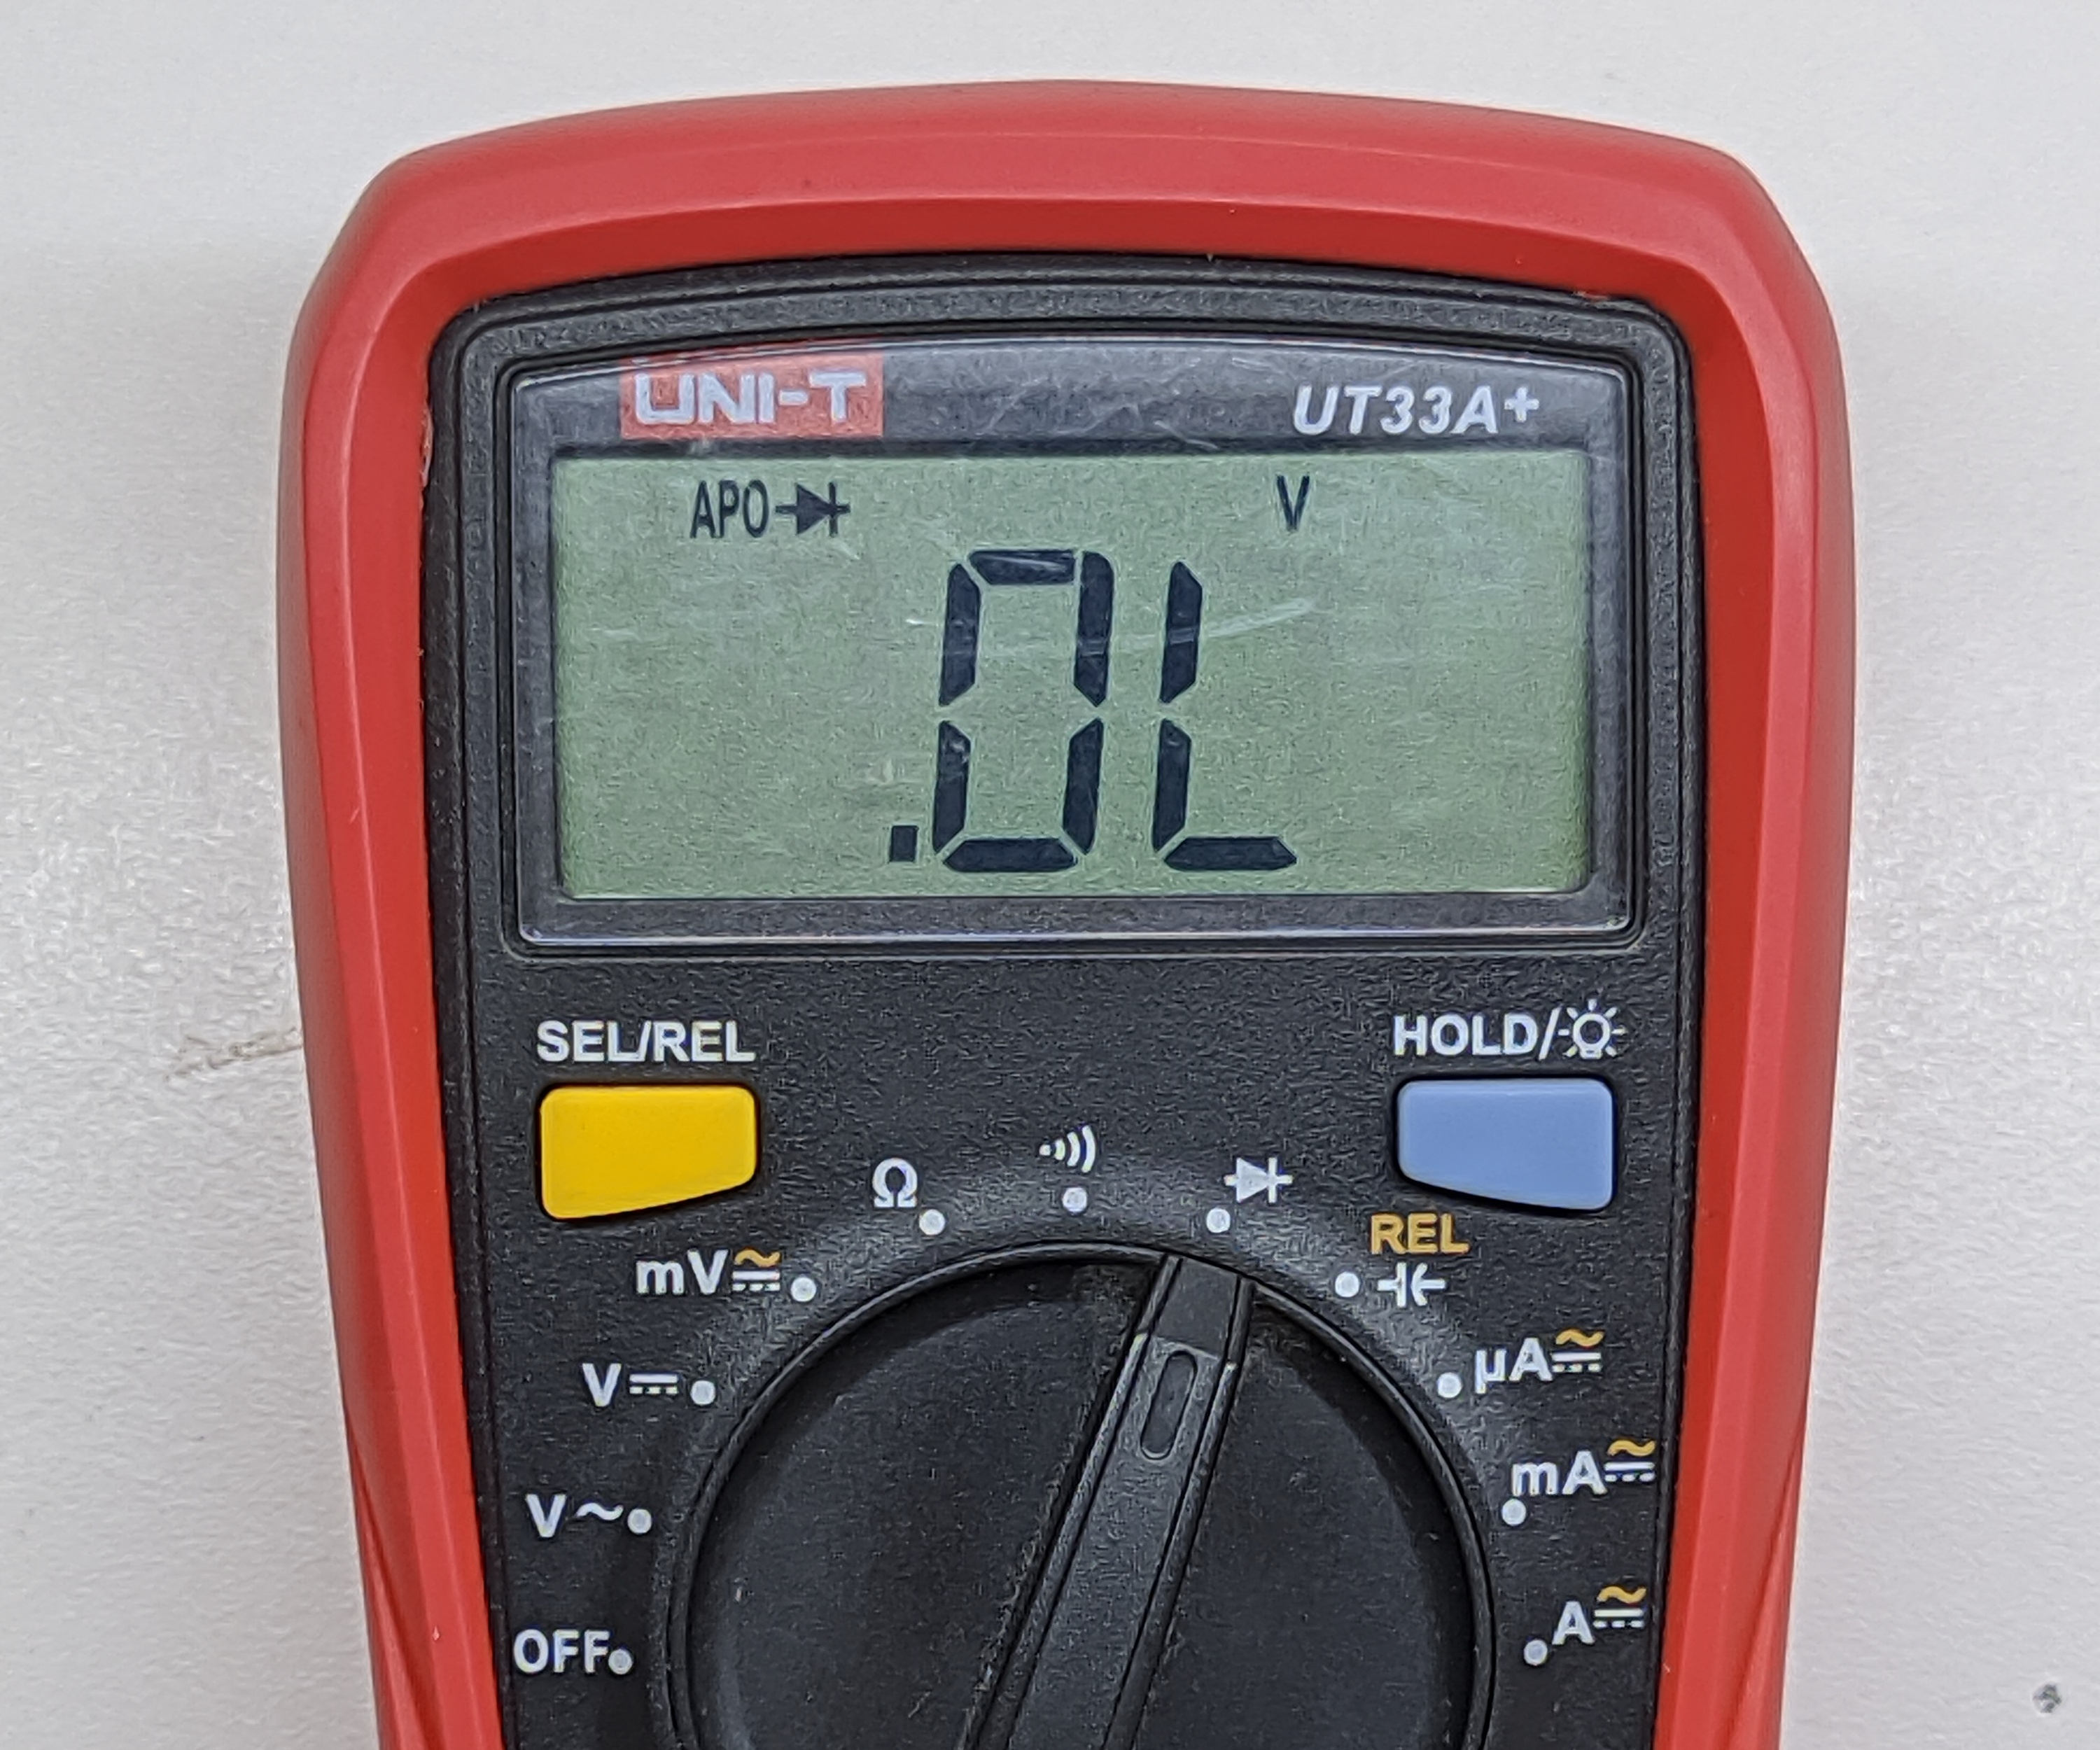
\includegraphics[width=1\textwidth]{pictures/mult_diod-i.jpg}
        \end{minipage}
        \begin{minipage}[b]{0.24\textwidth}
          \centering
          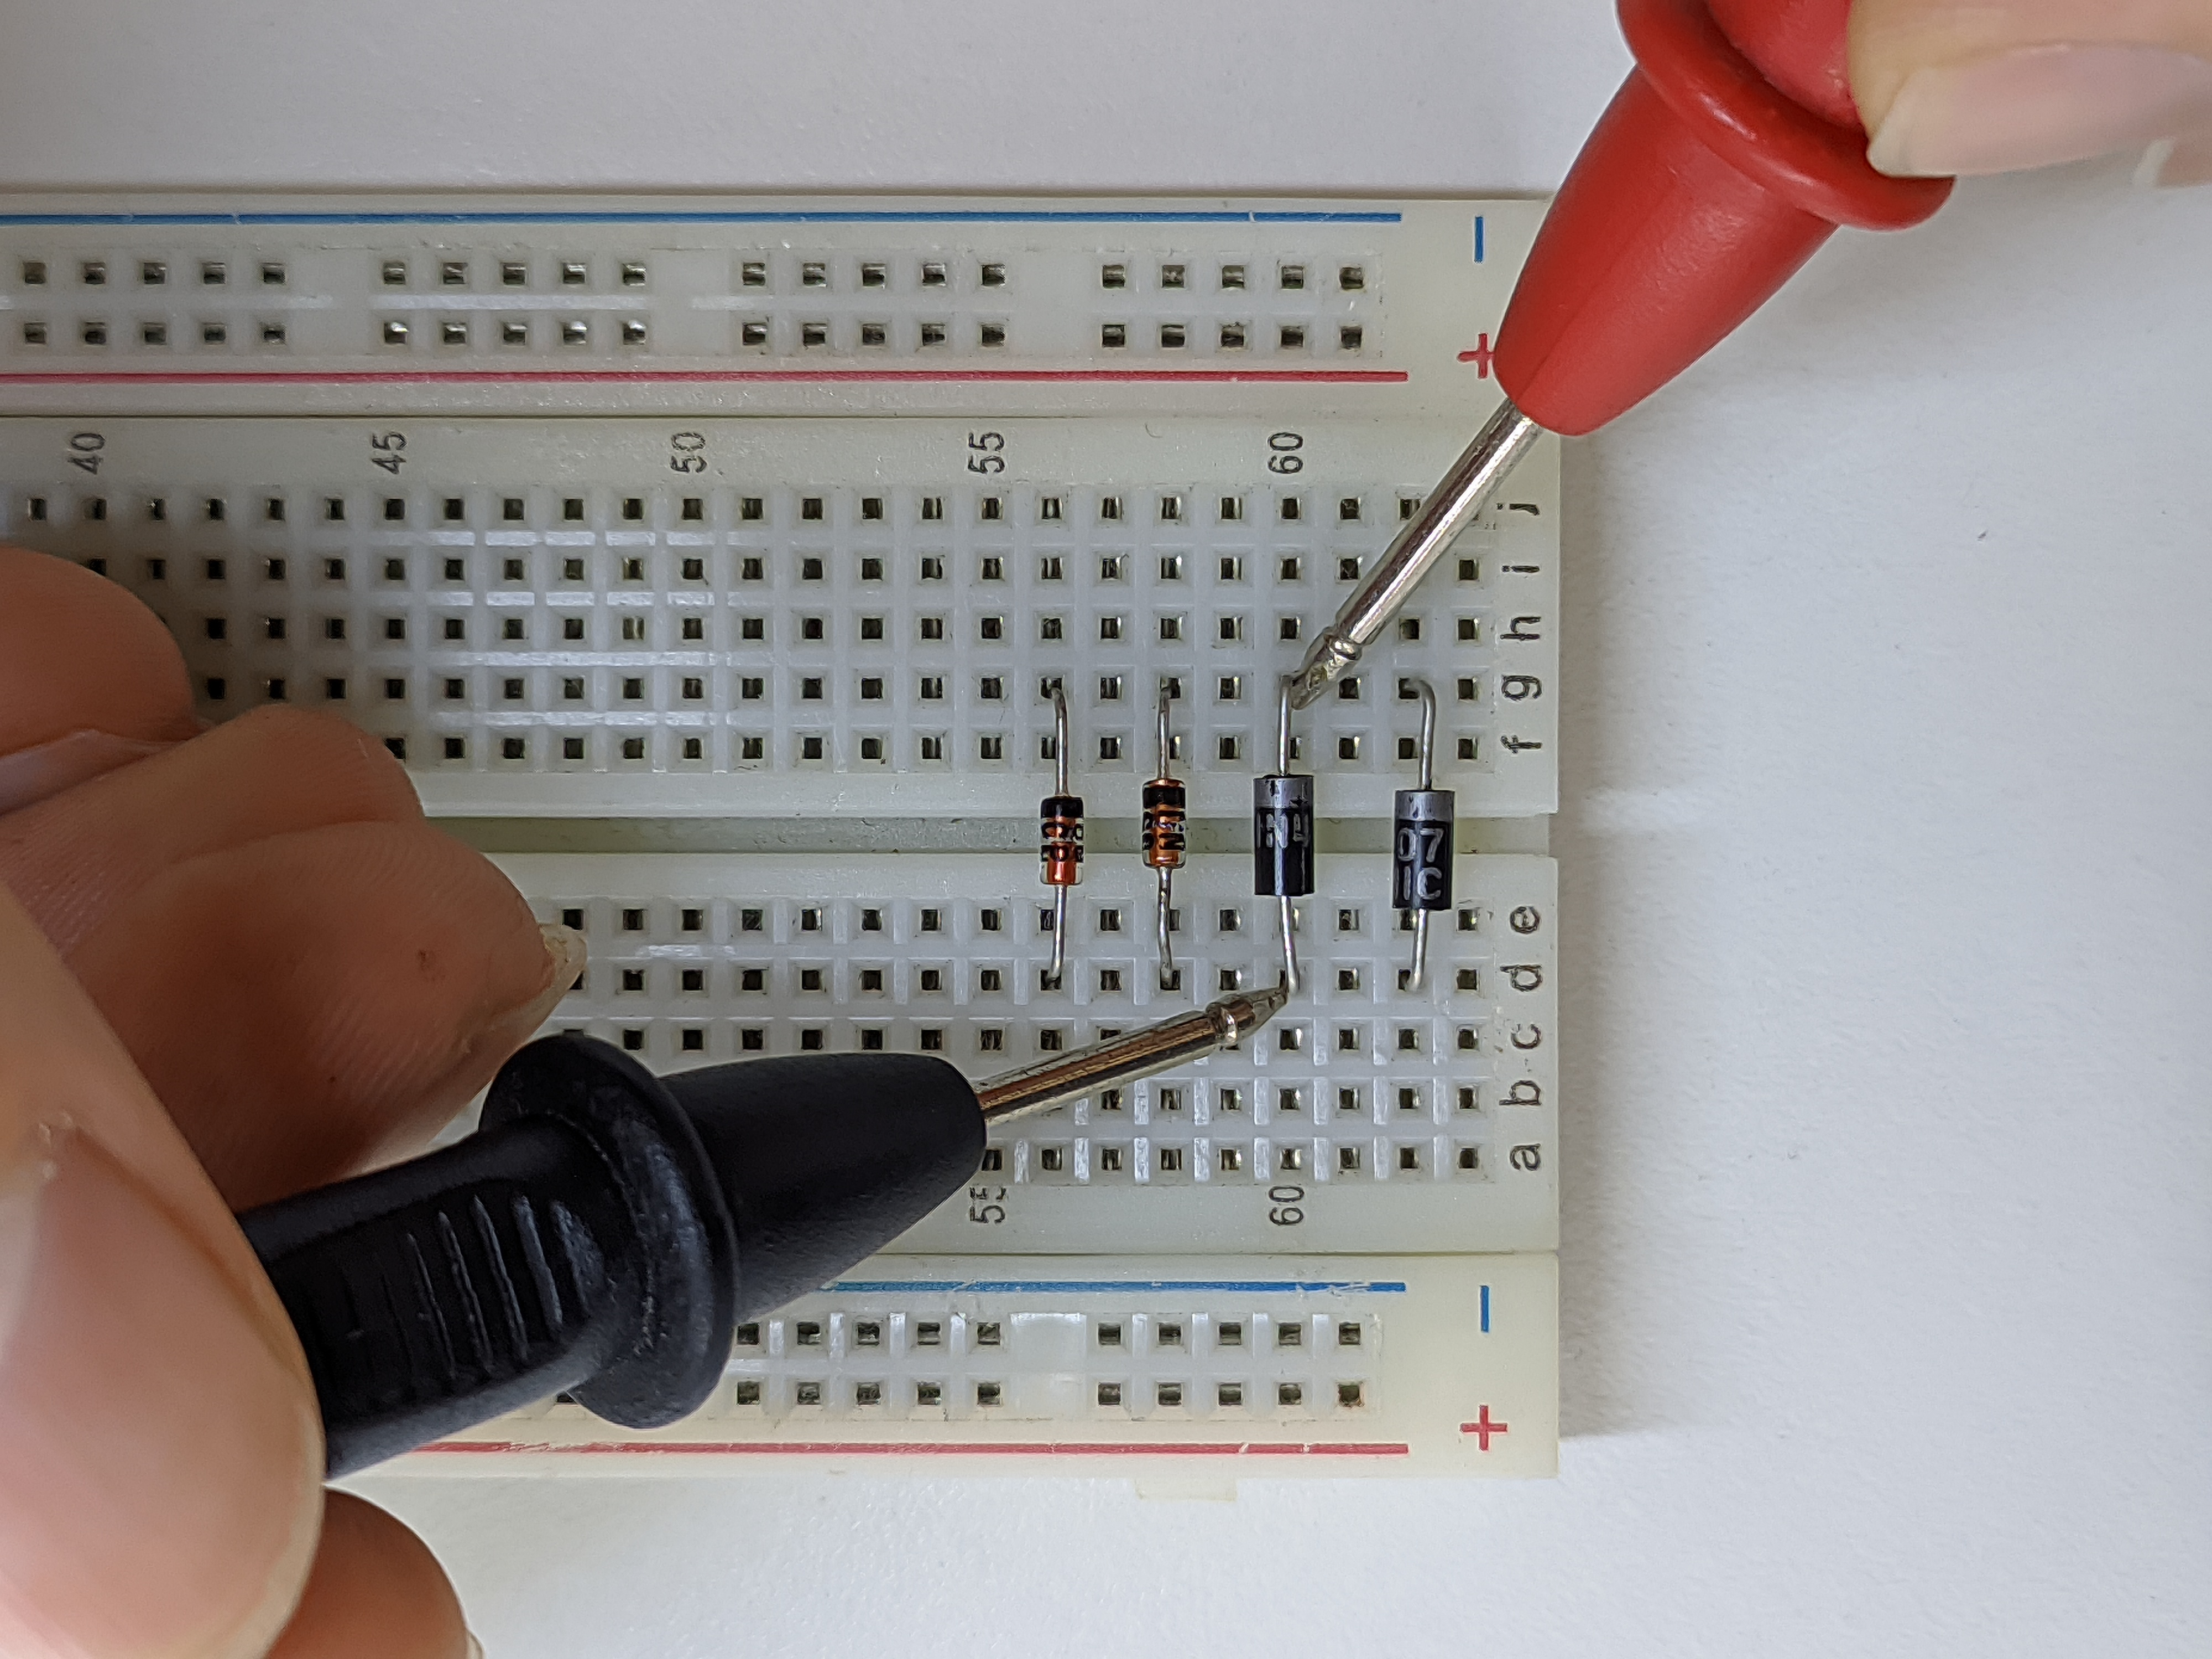
\includegraphics[angle=-90, width=1\textwidth]{pictures/prot_diod-2i.jpg}
          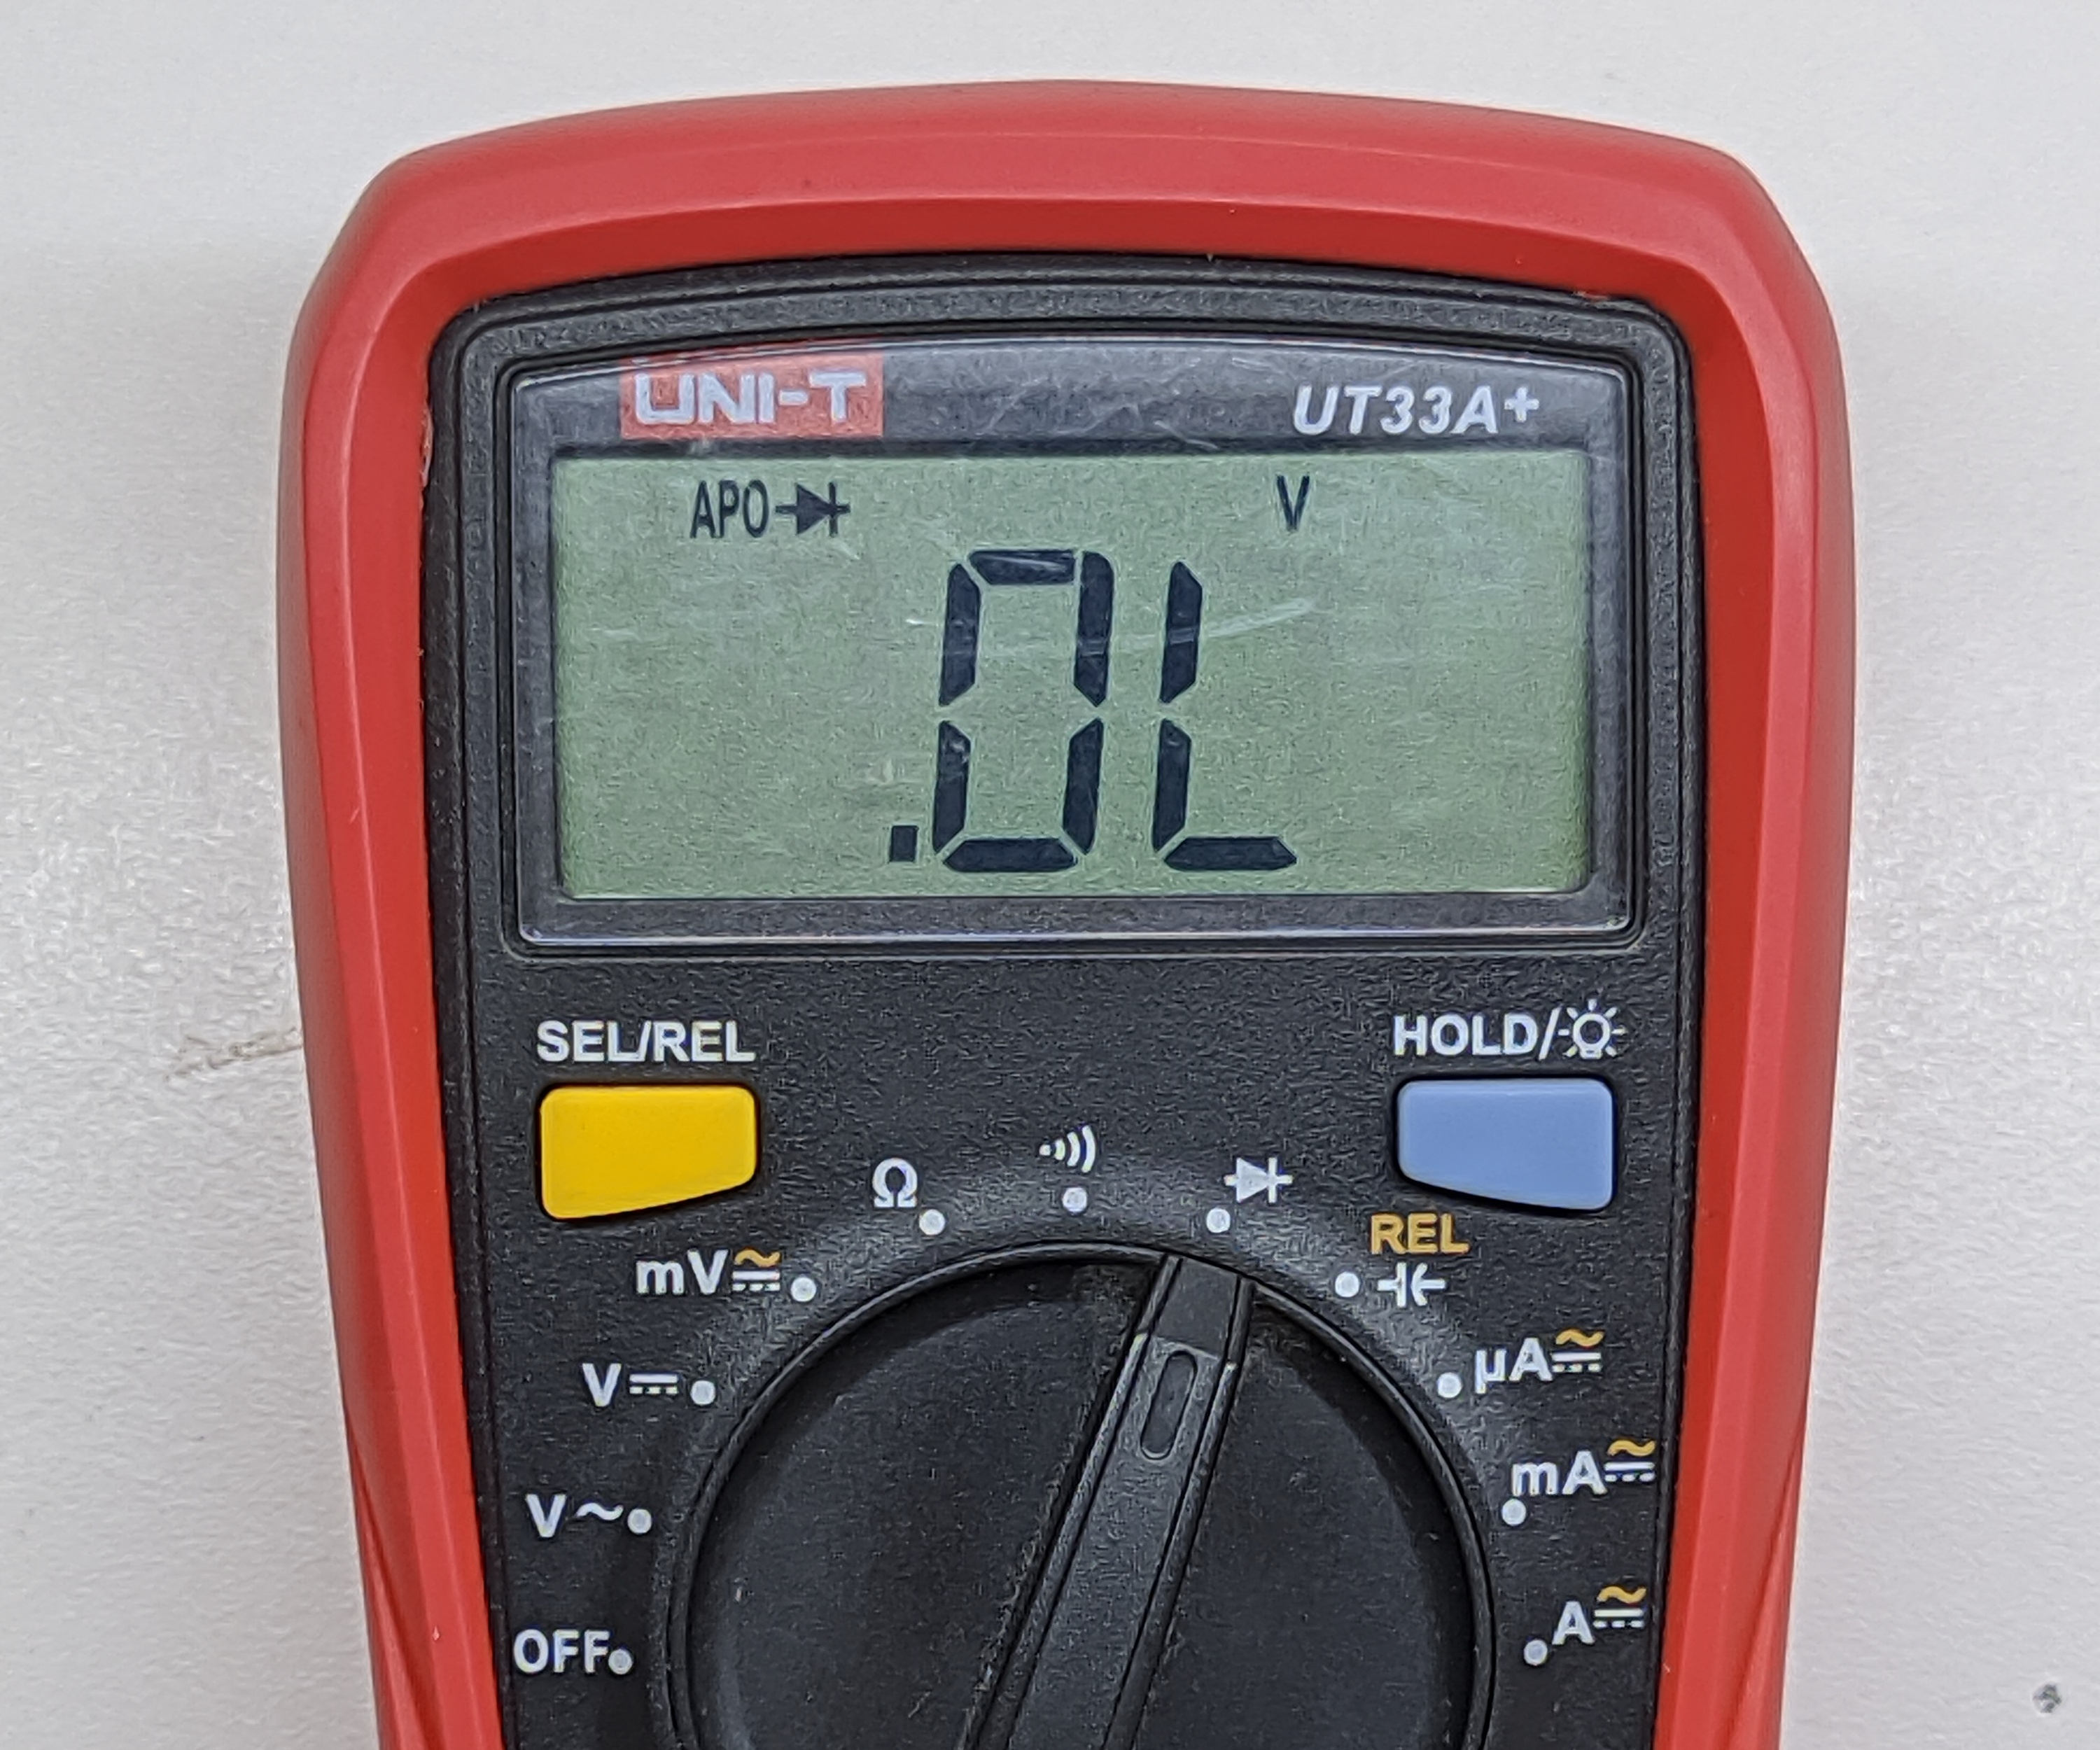
\includegraphics[width=1\textwidth]{pictures/mult_diod-i.jpg}
        \end{minipage}
        \begin{minipage}[b]{0.24\textwidth}
          \centering
          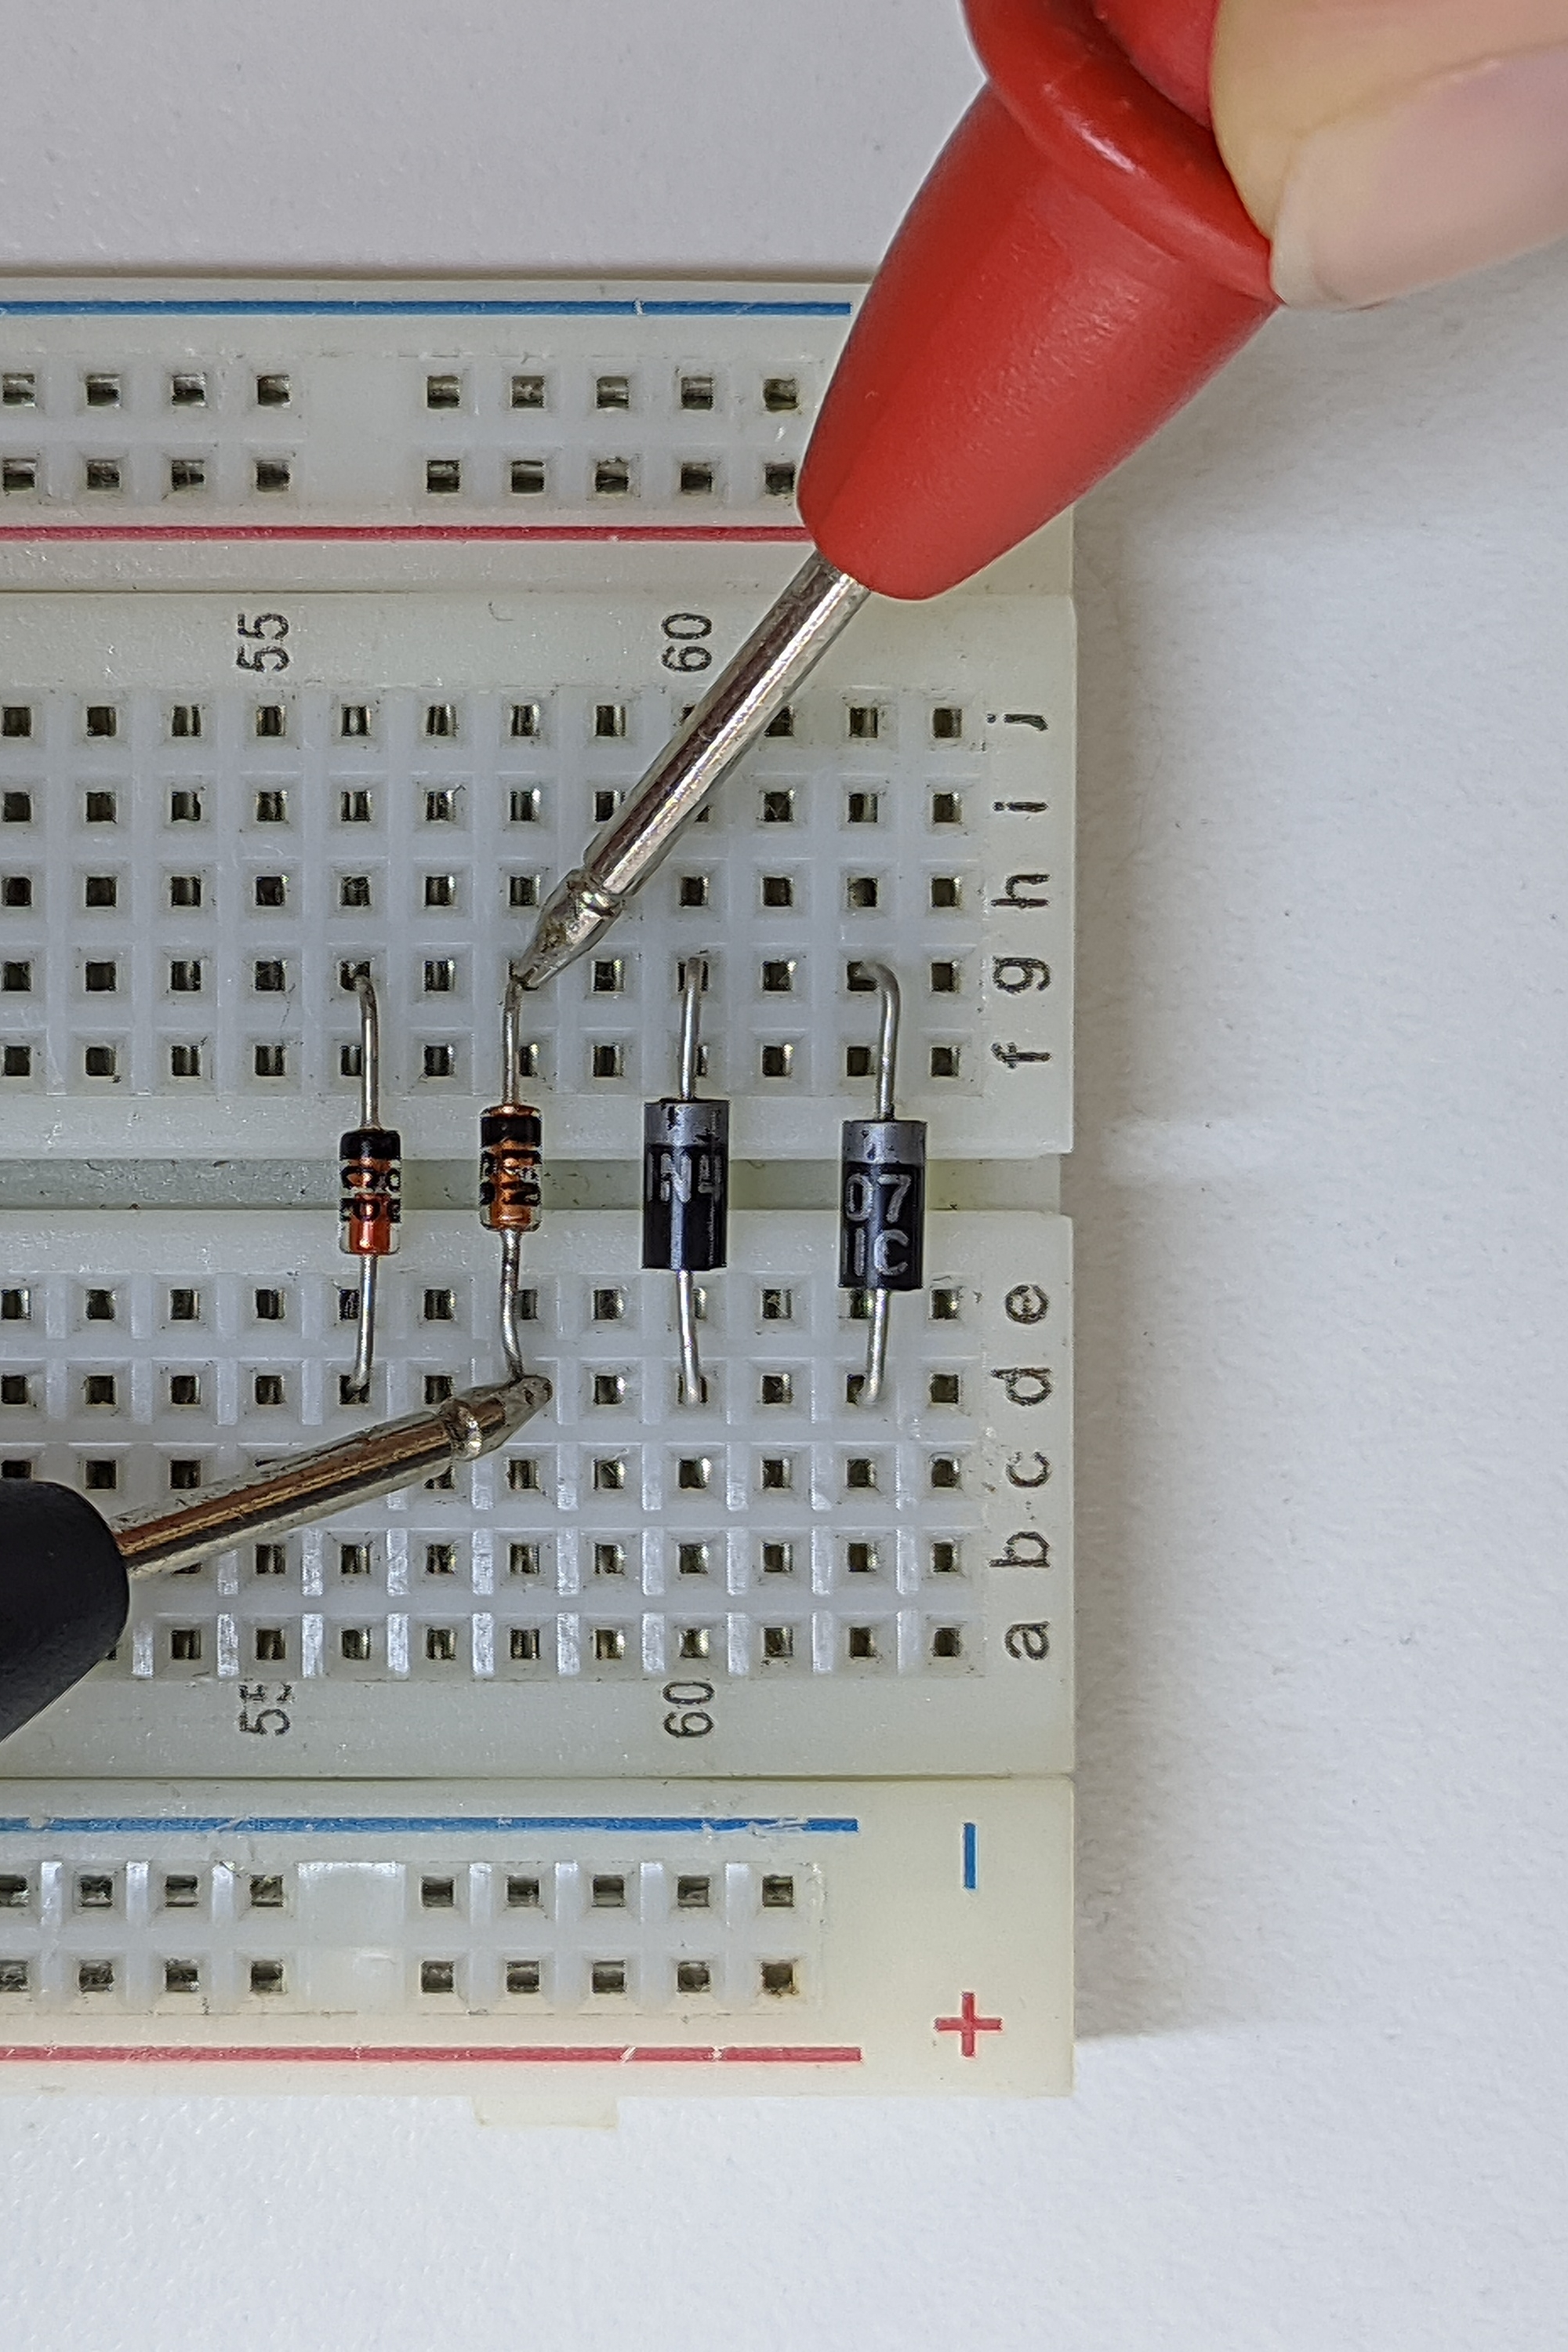
\includegraphics[angle=-90, width=1\textwidth]{pictures/prot_diod-3i.jpg}
          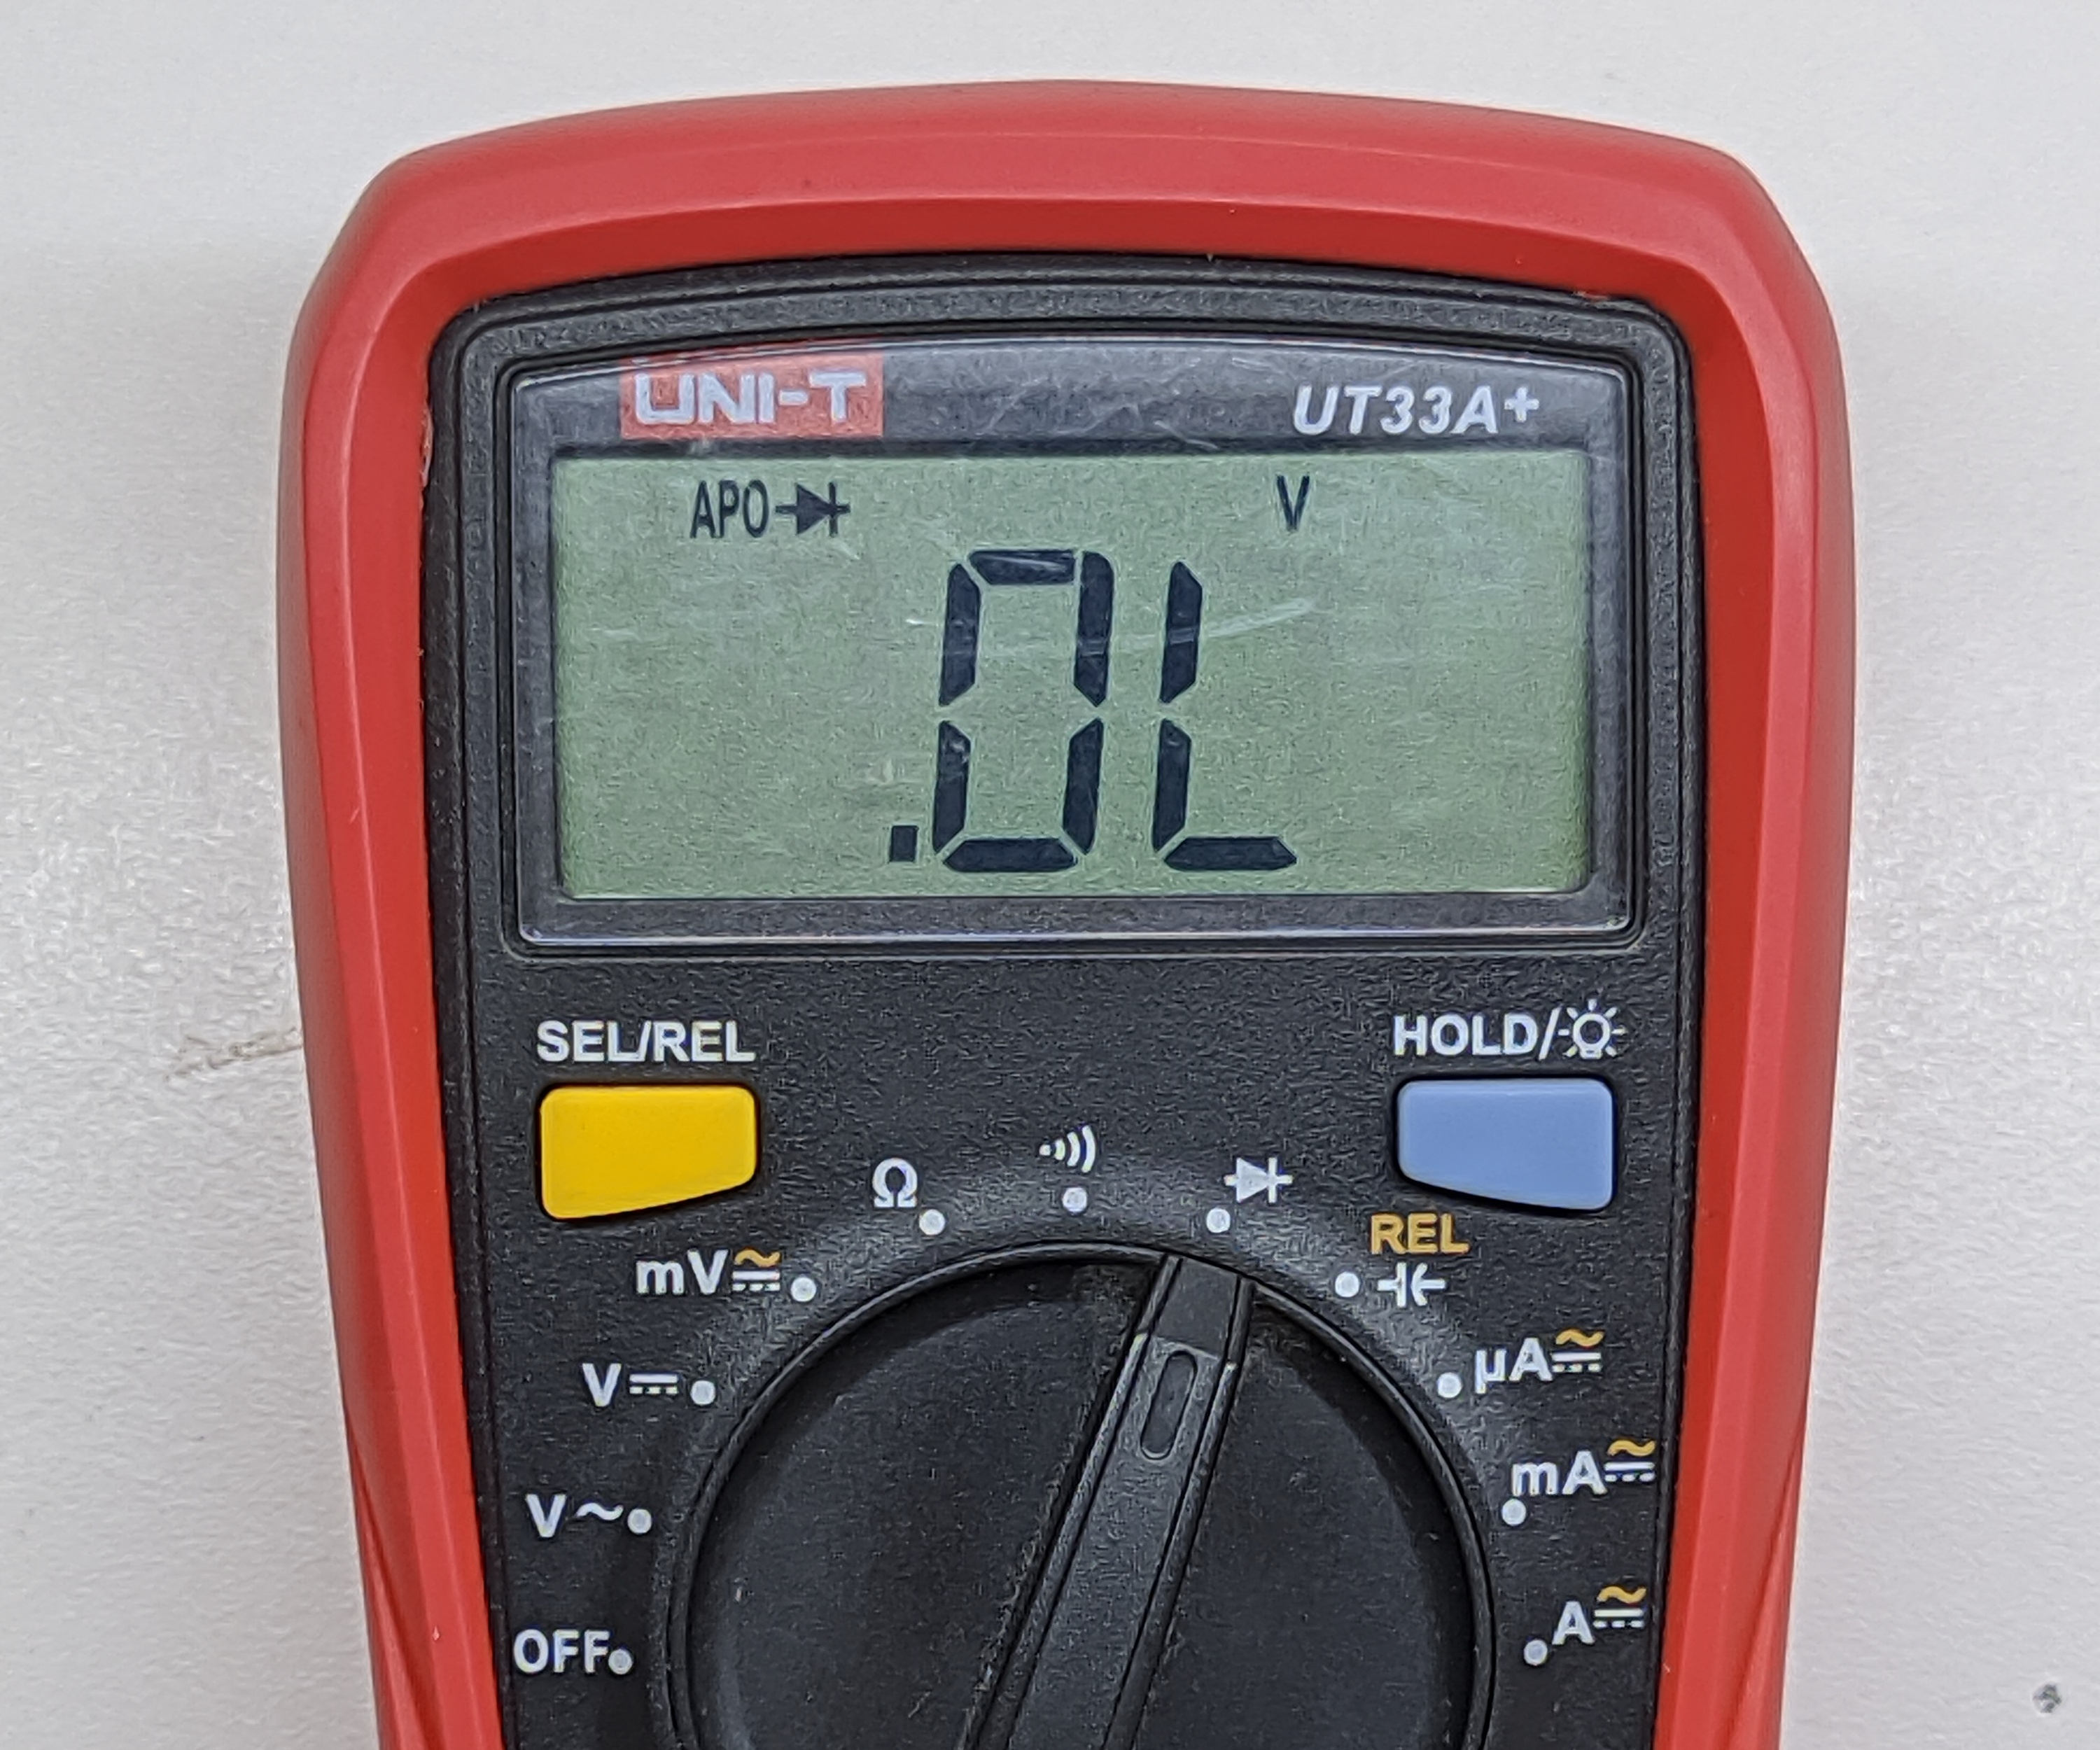
\includegraphics[width=1\textwidth]{pictures/mult_diod-i.jpg}
        \end{minipage}
        \begin{minipage}[b]{0.24\textwidth}
          \centering
          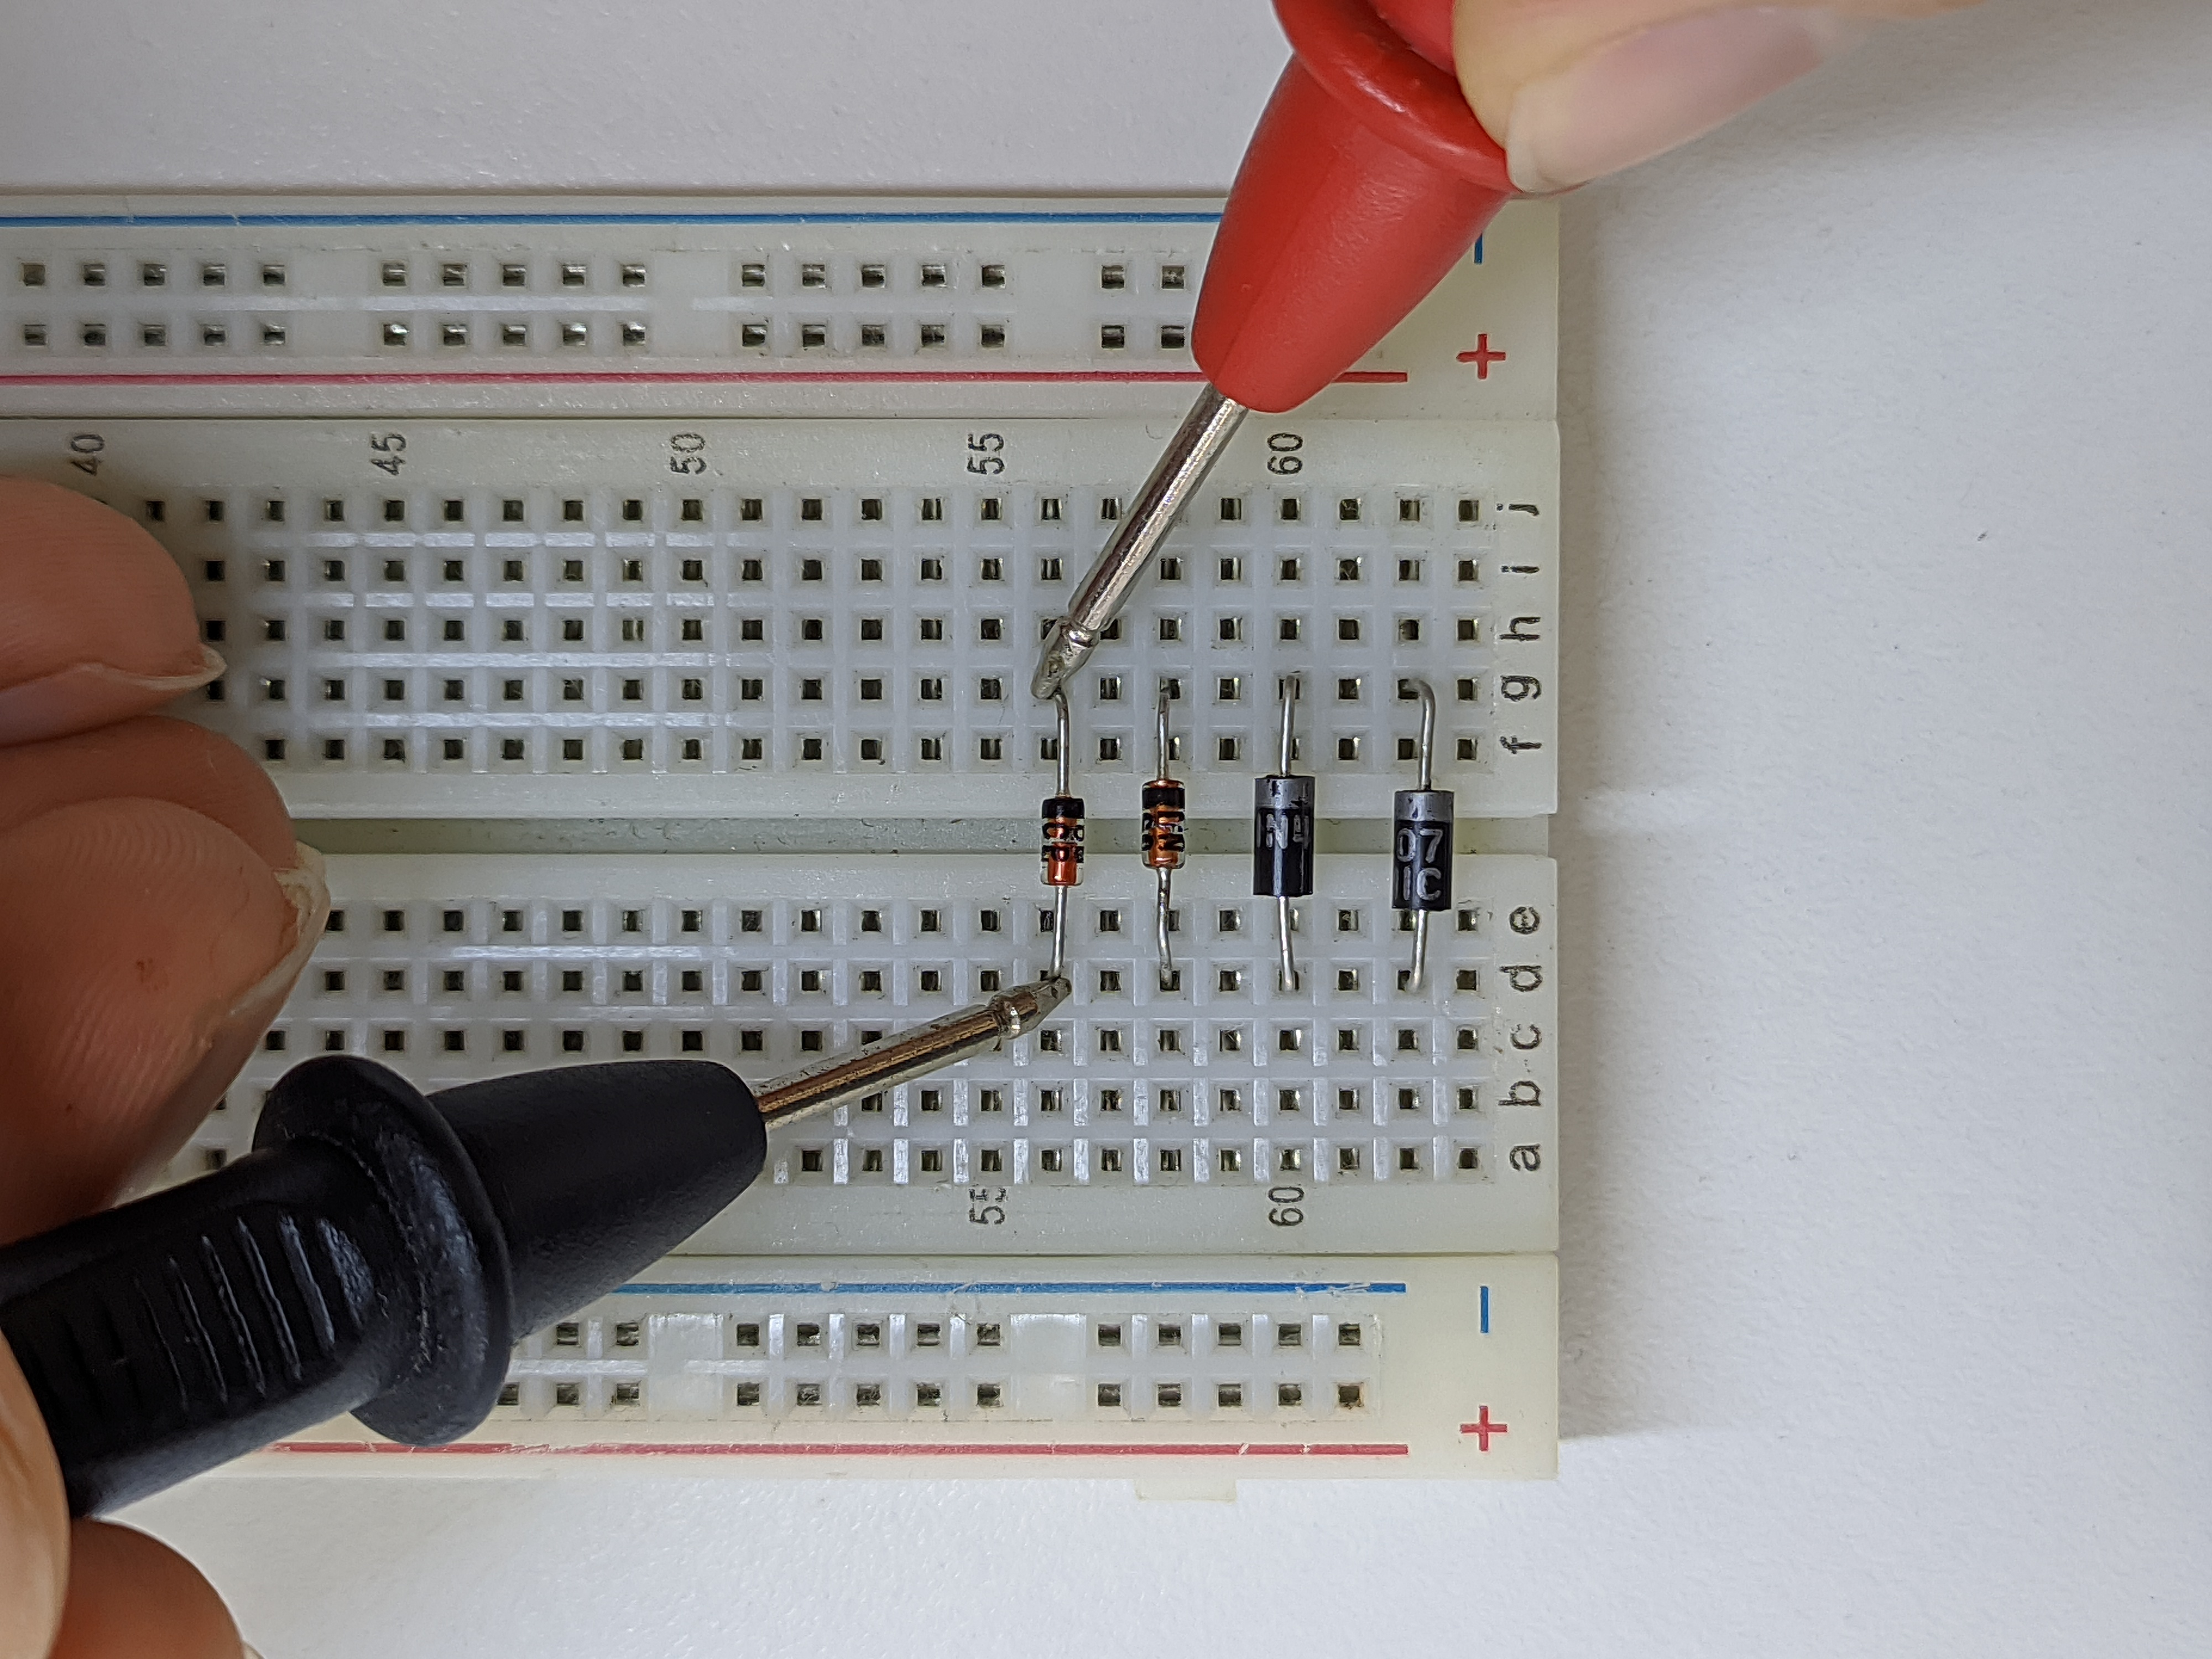
\includegraphics[angle=-90, width=1\textwidth]{pictures/prot_diod-4i.jpg}
          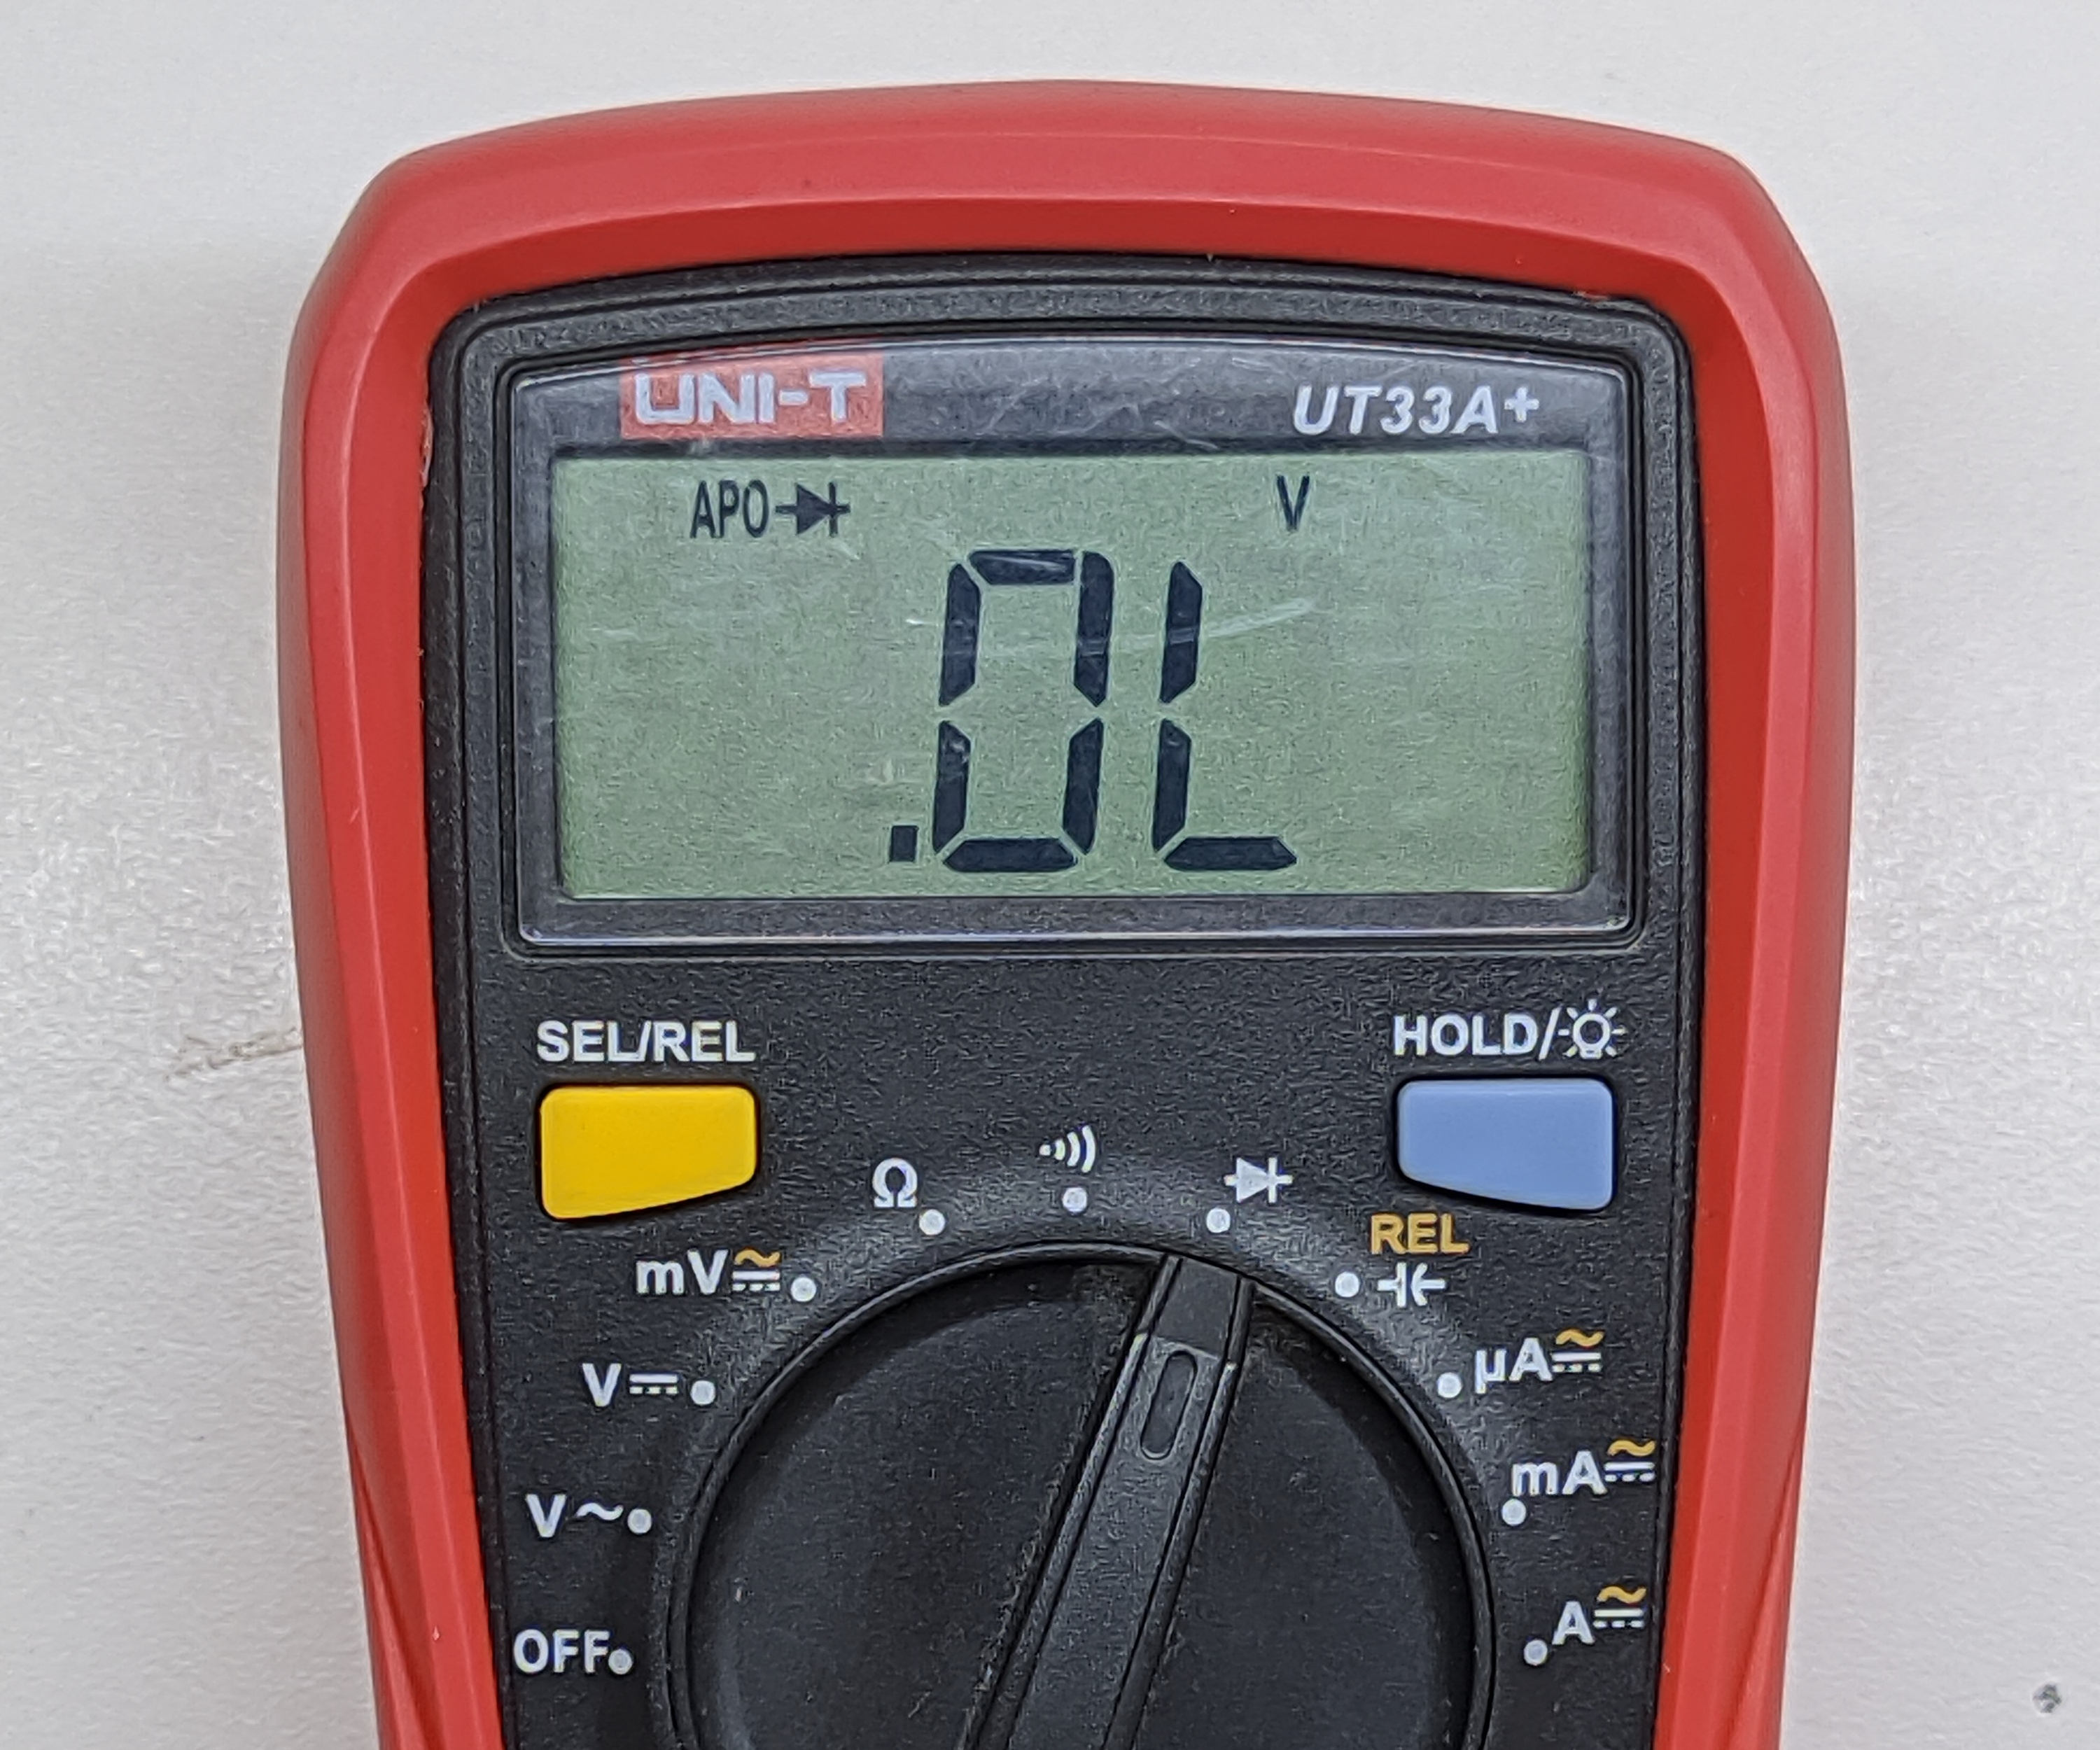
\includegraphics[width=1\textwidth]{pictures/mult_diod-i.jpg}
        \end{minipage}
      \end{subfigure}
    \end{figure}

    Despues de haber hecho todas las pruebas, se puede confeccionar la siguiente tabla:
    \begin{table}[H]
      \centering
      \begin{tabular}{|>{\centering\arraybackslash}m{3cm}|*{4}{>{\centering\arraybackslash}m{2cm}|}}
        \hline
        \textbf{Sentido de las puntas del multimetro} & \multicolumn{2}{c|}{\textbf{Diodo de germanio}} & \multicolumn{2}{c|}{\textbf{Diodo de silicio}} \\
        \cline{2-5}
        & \textbf{D1} & \textbf{D2} & \textbf{D1} & \textbf{D2} \\
        \hline

        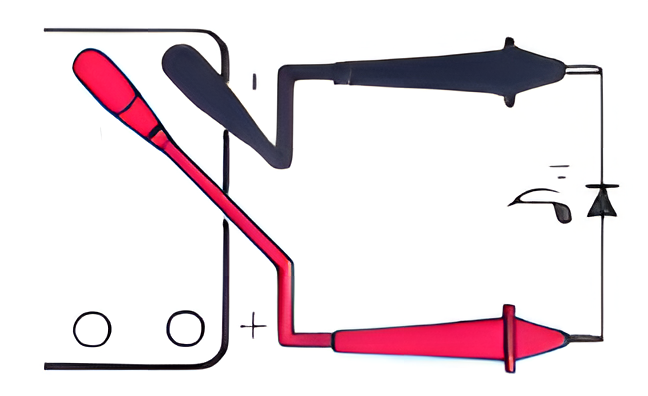
\includegraphics[height=1.8cm]{images/punta1.png} & $280\mV$ & $281\mV$ & $565\mV$ & $564\mV$ \\
        \hline
        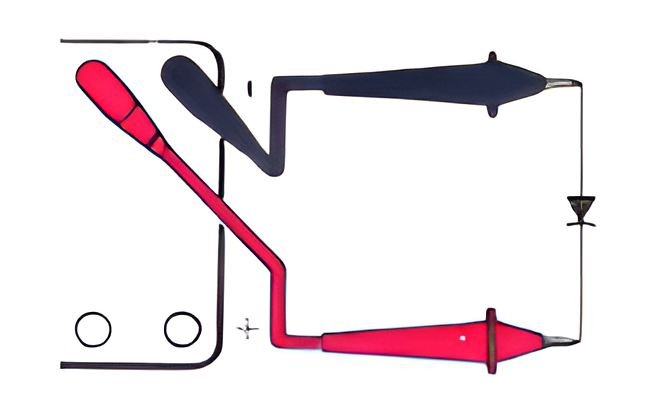
\includegraphics[height=1.8cm]{images/punta2.png} & OL & OL & OL & OL \\
        \hline
      \end{tabular}
      \caption{Mediciones con el multimetro en diferentes polaridades}
    \end{table}

    Queda claro que la marca negra en el empaquetado DO-35 y la marca plateada en el empaquetado DO-15 indican el
    catodo del diodo, y la parte que no tiene nada indica el anodo. Es importante destacar que, a pesar de que el
    procedimiento de dopado del diodo puede parecer un proceso totalmente controlado, esto no suele ser asi. El
    multimetro utilizado posiblemente no tiene buena resolucion para sacar estos desperfectos a flote, pero
    generalmente las caidas de tension suelen variar mas de un diodo a otro. Es posible que tambien hayamos tenido
    suerte, y que nos hayan tocado dos diodos de cada uno de los modelos, adyacentes uno de otro en la materia prima
    de la cual se fabricaron.

    Por otro lado, se puede apreciar que cuando polarizamos el diodo en inversa, el multimetro marcaba OL. Esto es la
    abreviatura para "carga abierta" (open load), lo que significa que para el multimetro, lo que estamos midiendo es
    lo mismo que un circuito que no esta cerrado.

    En cualquier caso, queda claramente definido cuales son los pines del diodo y cual es el comportamiento esperado
    de aqui en adelante.


  \chapter{Curva caracteristica del Diodo: Simulacion}
    La curva caracteristica del diodo permite establecer una relacion facil de entender entre la corriente que circula
    por el diodo y la caida de tension que se genera. Diferentes diodos tienen diferentes curvas caracteristicas, pero
    casi todas siguen la curva exponencial definida como:

    \begin{equation}
      i_D = I_0 \left(e^{\frac{v_d}{V_T}} - 1 \right)
      \label{eq.caracteristica}
    \end{equation}

    Las variaciones suelen estar en el termino $I_0$ que es la corriente de polarizacion en inversa, y el termino $V_T$
    que es la variacion de voltaje por grado celsius.

    \section{Polarizacion en directa}
      La polarizacion en directa del diodo implica que la region de empobrecimiento del diodo se contraiga a causa del
      potencial colocado en el diodo. Este potencial, que tiene un flujo de corriente convencional que ingresa por la
      region P y egresa por la region N (en flujo no convencional, los $e^-$ ingresan por N y egresan por P). Este
      flujo de corriente provoca que haya un exceso de portadores mayoritarios en la region P, haciendo que aquellos
      que tienen suficiente energia potencial puedan sobrepasar la region de empobrecimiento, recombinandose con los
      portadores mayoritarios de la region N y generando un movimiento de cargas. Esto pasa tambien en la region N.

      A medida que mas portadores mayoritarios fluyen, mas se contrae la region de empobrecimiento, causando que los
      portadores mayoritarios requieran menos potencial para sobrepasar la barrera. Este fenomeno es por el cual el
      diodo va teniendo menos "resistencia equivalente" a medida que el voltaje o la corriente aumentan.

      \subsection{Diodo de Silicio}
        Para corroborar la curva caracteristica del diodo de silicio, y como esta responde a los cambios de voltaje, se
        creo un circuito en el software LTSpice muy basico para probar la polarizacion del diodo de silicio.

        El programa, de manera automatica, genera un barrido de tension que arranca en los $-2V$ y termina en los $10V$,
        haciendo pasos de $100mV$ por muestra. De esta forma hay suficiente resolucion para considerarla una buena
        aproximacion de la curva caracteristica del diodo.

        Se selecciono el diodo 1N4007 como diodo de pruebas de silicio y $R_1 = 1K\Omega$. El circuito armado en
        LTSpice se puede ver en figura (\ref{crkt.Si.directa}) y se han empleado las directivas mostradas en el
        listado (\ref{list.Si.directa}) para la simulacion.

        \begin{figure}[H]
          \centering
          \begin{minipage}{0.45\textwidth}
            \begin{circuitikz}[american voltages]
              \draw (0, -1) to [V=$V_1$, invert]             (0, 3)
                            to [short, -, i>^=$i_D$]         (1, 3)
                            to [R=$R_1$, v=$V_{R_1}$]        (4, 3)
                            to [short, -]                    (5, 3)
                            to [D=$1N4007$, v=$v_D$]         (5, -1)
                            to [short, -]                    (5, -1)
                            to [short, -]                    (0, -1)
                            ;
            \end{circuitikz}
            \caption{Circuito con diodo de silicio 1N4007.}
            \label{crkt.Si.directa}
          \end{minipage}
          \hfill
          \begin{minipage}{0.45\textwidth}
            \begin{lstlisting}[style=ltspice, caption={Parámetros de simulación LTspice}, label=list.Si.directa]
              .dc V1 -2 10 100m
            \end{lstlisting}
          \end{minipage}
        \end{figure}

        Habiendo simulado el circuito anterior, se extrayeron los resultados para ser mostrados en la figura
        (\ref{graph.simulation.Si.directa}).

        \begin{figure}[!ht]
          \centering
          \begin{minipage}{0.45\textwidth}
            \begin{tikzpicture}
              \begin{axis}[
                width=7cm,
                height=5.5cm,
                xlabel={$v_D$ [V]},
                ylabel={$i_D$ [mA]},
                grid=both,
                minor tick num=1,
                scale only axis,
                enlargelimits=false,
                extra x ticks={0.7},
                extra x tick style={
                  grid style={red, thick, dashed},
                  tick style={red},
                  tick label style={red}
                 },
                scaled ticks=false,
                restrict x to domain=0:4,
              ]
              \addplot[
                color=blue,
                mark=none,
                thick,
              ] table[
                col sep=tab,
                header=true,
                x=V(d1),
                y expr=\thisrow{I(D1)}*1000
              ] {simulations/TP2_1_graph.txt};
              \end{axis}
            \end{tikzpicture}
            \caption{Grafico de la curva caracteristica del simulador.}
            \label{graph.simulation.Si.directa}
          \end{minipage}
          \hfill
          \begin{minipage}{0.45\textwidth}
            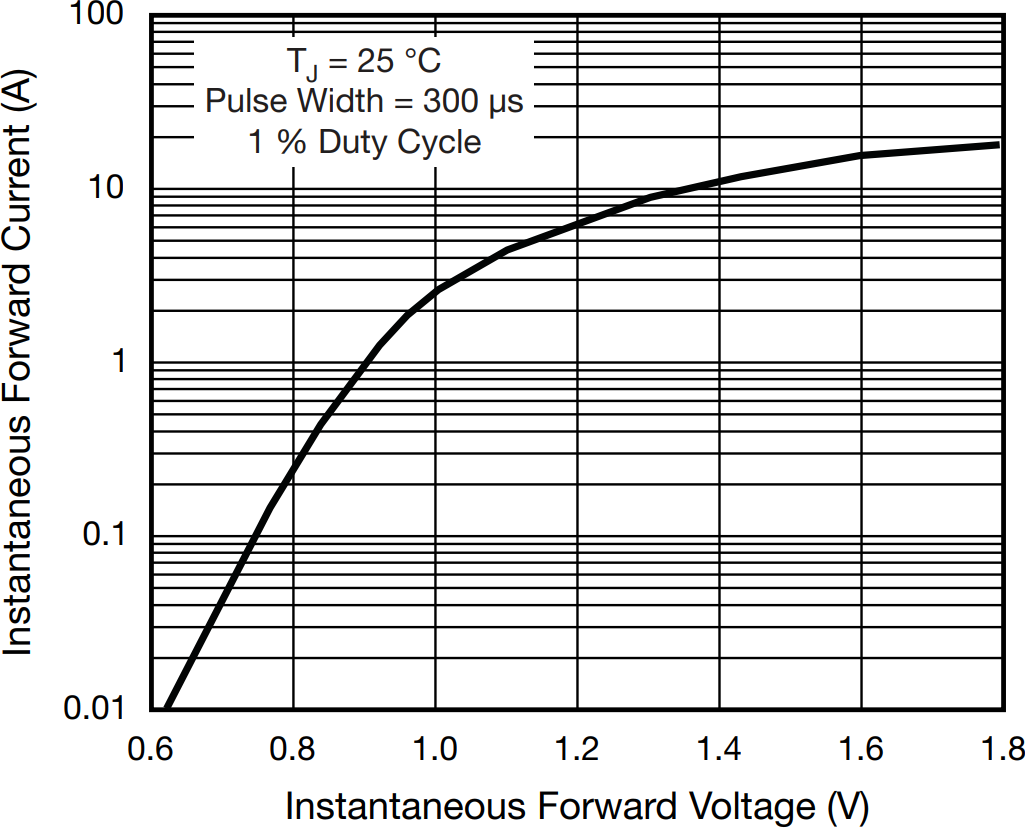
\includegraphics[width=1\textwidth]{images/Curva_Datash_Si_dir.png}
            \caption{Grafico de la curva caracteristica de la hoja de datos.}
            \label{graph.datasheet.Si.directa}
          \end{minipage}
        \end{figure}

        Se puede observar que la grafica proveniente de la hoja de datos del diodo de silicio \cite{DS0} es muy poco
        similar a la obtenida con la simulacion. Esto se debe a que el analisis de baja corriente/voltaje que se esta
        haciendo para este trabajo practico no suele ser importante (por lo menos para el diodo seleccionado) debido a
        que el rango operativo esta a mas de 100 veces la corriente (por eso la escala es logaritmica) a la que se
        sometido el diodo en la simulacion.

        De todas formas, se puede apreciar que el "codo de conmutacion" efectivamente ocurre a los 0.7V en ambas
        graficas. Se puede apreciar con mayor presicion en el grafico simulado la curva de corriente la cual
        el diodo experimenta cuando pasa de no estar polarizado a cuando conduce. En la grafica del fabricante, se
        puede apreciar mejor, como es que lo que se ve en la simulacion como una rampa lineal, en altas
        corrientes en realidad no es tan lineal, y empieza a experimentar un aumento de la "resistencia equivalente"
        debido a la proximidad con el limite operativo del diodo.

      \subsection{Diodo de Germanio}
        Para corroborar la curva caracteristica del diodo de germanio, y como esta responde a los cambios de voltaje,
        nuevamente se creo un circuito en el software LTSpice muy basico para probar la polarizacion del diodo de
        germanio. El programa, realiza el mismo barrido que para el circuito del diodo de silicio con la misma
        resolucion.

        Se selecciono el diodo 1N60 como diodo de pruebas de germanio y $R_1 = 1K\Omega$. El circuito armado en
        LTSpice se puede ver en figura (\ref{crkt.Ge.directa}) y se han empleado las directivas mostradas en el
        listado (\ref{list.Ge.directa}) para la simulacion.

        \begin{figure}[!ht]
          \centering
          \begin{minipage}{0.45\textwidth}
            \begin{circuitikz}[american voltages]
              \draw (0, -1) to [V=$V_1$, invert]             (0, 3)
                            to [short, -, i>^=$i_D$]         (1, 3)
                            to [R=$R_1$, v=$V_{R_1}$]        (4, 3)
                            to [short, -]                    (5, 3)
                            to [D=$1N60$, v=$v_D$]           (5, -1)
                            to [short, -]                    (5, -1)
                            to [short, -]                    (0, -1)
                            ;
            \end{circuitikz}
            \caption{Circuito con diodo de silicio 1N4007.}
            \label{crkt.Ge.directa}
          \end{minipage}
          \hfill
          \begin{minipage}{0.45\textwidth}
            \begin{lstlisting}[style=ltspice, caption={Parámetros de simulación LTspice}, label=list.Ge.directa]
              .dc V1 -2 10 100m
              .model 1N60 D (RS=50.0559 EG=1.11 XTI=3 VJ=0.8 M=0.1 FC=0.5 BV=40 CJO=1.75p IS=1.37773u N=2 TT=100n type=germanium)
            \end{lstlisting}
          \end{minipage}
        \end{figure}

        Los resultados de la simulacion estan presentes en la figura (\ref{graph.simulation.Ge.directa}).

        \begin{figure}[!ht]
          \centering
          \begin{minipage}{0.45\textwidth}
            \begin{tikzpicture}
              \begin{axis}[
                width=7cm,
                height=5.5cm,
                xlabel={$v_D$ [V]},
                ylabel={$i_D$ [mA]},
                grid=both,
                minor tick num=1,
                scale only axis,
                enlargelimits=false,
                extra x ticks={0.3},
                extra x tick style={
                  grid style={red, thick, dashed},
                  tick style={red},
                  tick label style={red}
                 },
                scaled ticks=false,
                restrict x to domain=0:4,
              ]
              \addplot[
                color=blue,
                mark=none,
                thick,
              ] table[
                col sep=tab,
                header=true,
                x=V(d1),
                y expr=\thisrow{I(D1)}*1000
              ] {simulations/TP2_2_graph.txt};
              \end{axis}
            \end{tikzpicture}
            \caption{Grafico de la curva caracteristica del simulador.}
            \label{graph.simulation.Ge.directa}
          \end{minipage}
          \hfill
          \begin{minipage}{0.45\textwidth}
            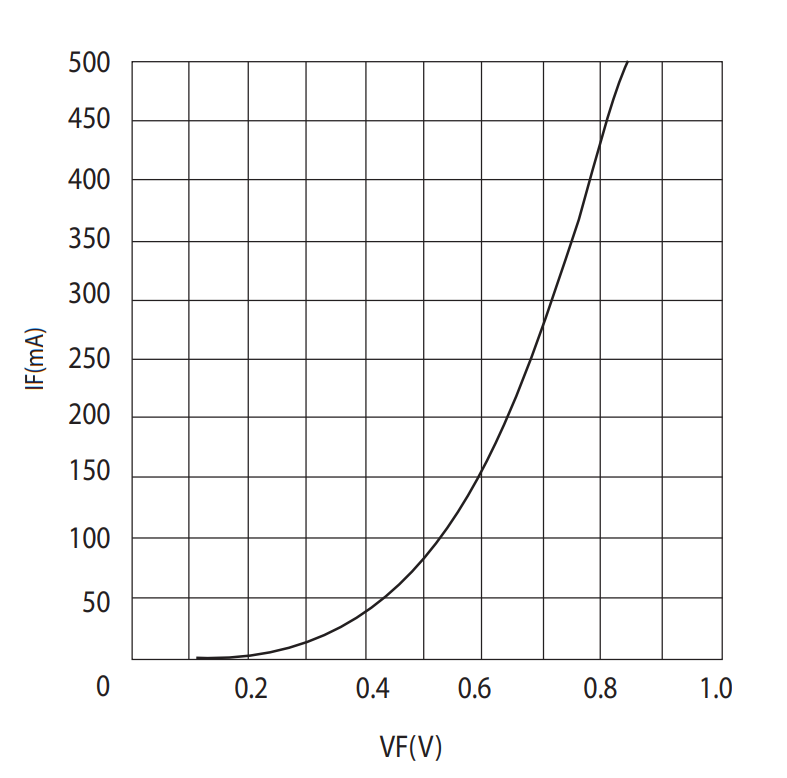
\includegraphics[width=1\textwidth]{images/Curva_Datash_Ge_dir.png}
            \caption{Grafico de la curva caracteristica de la hoja de datos.}
            \label{graph.datasheet.Ge.directa}
          \end{minipage}
        \end{figure}

        Se puede observar que, a diferencia del diodo de silicio, la grafica provista por la hoja de datos del diodo de
        germanio \cite{DS1} tiene mas correlacion con los datos simulados. Se puede apreciar que el "codo de
        conmutacion" ocurre mas o menos a los $0.3V$ en ambos graficos. Ademas, debido a que el diodo es de menor
        potencia, la grafica tiene valores un poco mas proximos a los que realizamos en las pruebas con el simulador
        respecto al 1N4007.

      \subsection{Comparacion de ambas simulaciones}

        \begin{figure}[!ht]
          \centering
          \begin{tikzpicture}
            \begin{axis}[
              width=14cm,
              height=7cm,
              xlabel={$v_D$ [V]},
              ylabel={$i_D$ [mA]},
              grid=both,
              minor tick num=1,
              scale only axis,
              enlargelimits=false,
              scaled ticks=false,
              restrict x to domain=-0.2:1.4,
            ]
            \addplot[
              color=blue,
              mark=none,
              thick,
            ] table[
              col sep=tab,
              header=true,
              x=V(d1),
              y expr=\thisrow{I(D1)}*1000
            ] {simulations/TP2_1_graph.txt};
            \addlegendentry{Si}
            \addplot[
              color=red,
              mark=none,
              thick,
            ] table[
              col sep=tab,
              header=true,
              x=V(d1),
              y expr=\thisrow{I(D1)}*1000
            ] {simulations/TP2_2_graph.txt};
            \addlegendentry{Ge}
            \end{axis}
          \end{tikzpicture}
          \caption{Grafico de las curvas caracteristicas simuladas de los diodos de Silicio y Germanio utilizados.}
          \label{graph.simulation.comparativa.directa}
        \end{figure}

        En la figura (\ref{graph.simulation.comparativa.directa}) se puede apreciar una clara diferencia en cuanto al voltaje
        necesario para lograr poner los diodos en conduccion, siendo la de Germanio alrededor de los $0.2V$ a $0.3V$
        mientras que el de Silicio se encuentra entre $0.6V$ a $0.7V$. Esta diferencia en el codo de conmutacion se
        debe principalmente al potencial de umbral impuesto por la region de empobrecimiento. Los portadores
        mayoritarios de cada region pueden estar circulando libremente por su region, pero mientras que su energia
        sea menor a la energia potencial umbral, estos no seran recombinados en su region opuesta y no habra flujo de
        portadores. La variacion del potencial umbral es debido a la energia necesaria para que un electron en la capa
        de valencia sea repelido de su atomo.

        El menor requerimiento de energia en los diodos de Germanio, implica que el potencial que se debe aplicar en los
        terminales del diodo es menor, lo que puede significar un beneficio en polarizacion directa, pero como se vera
        mas adelante, puede implicar una complicacion en polarizacion inversa.

    \section{Polarizacion en inversa}
      La polarizacion en inversa del diodo implica que la region de empobrecimiento del mismo se dilate a causa del
      potencial aplicado a los terminales del diodo. Este potencial genera que los portadores mayoritarios en vez de
      querer acercarce a la region de empobrecimiento, quieran acercarse a los terminales de cada region. Esto, en
      efecto produce que la region de empobrecimiento se ensanche debido a la fuerza de atraccion causada por la
      diferencia de potencial de signo opuesto.

      A medida que se aumente el potencial inverso, mayor va a ser la atraccion que perciben los portadores
      mayoritarios a los terminales respectivos, y mayor va a ser el ensanchamiento de la region de empobrecimiento.
      A pesar de que practicamente no va a haber flujo de portadores mayoritarios en el diodo, hay un flujo de
      portadores minoritarios. Ese flujo esta dictado por la ecuacion (\ref{eq.caracteristica}), que si consideramos
      el termino exponencial proximo a cero por el exponente negativo, quedaria:
      \begin{equation*}
        i_D = -I_0
      \end{equation*}

      Llega un momento en el que el potencial inverso sobrepasa las capacidades fisicas del diodo, generando la
      ruptura de la union PN y destruyendo el diodo.

      \subsection{Diodo de Silicio}
        Para corroborar la curva caracteristica en inversa del diodo de silicio, y como esta responde a los cambios de
        voltaje, se creo un circuito en el software LTSpice muy basico para probar la polarizacion del diodo de
        silicio.

        El programa, de manera automatica, genera un barrido de tension que arranca en los $-1200V$ y termina en los
        $10V$, haciendo pasos de $100mV$ por muestra. De esta forma hay suficiente resolucion para considerarla una
        buena aproximacion de la curva caracteristica en inversa del diodo.

        Se selecciono nuevamente el diodo 1N4007 como diodo de pruebas de silicio y $R_1 = 1K\Omega$. El circuito
        armado en LTSpice se puede ver en figura (\ref{crkt.Si.inversa}) y se han empleado las directivas mostradas
        en el listado (\ref{list.Si.inversa}) para la simulacion.

        \begin{figure}[!ht]
          \centering
          \begin{minipage}{0.45\textwidth}
            \begin{circuitikz}[american voltages]
              \draw (0, -1) to [V=$V_1$]                     (0, 3)
                            to [short, -, i<^=$i_D$]         (1, 3)
                            to [R=$R_1$, v<=$V_{R_1}$]       (4, 3)
                            to [short, -]                    (5, 3)
                            to [D=$1N4007$, v<=$v_D$]        (5, -1)
                            to [short, -]                    (5, -1)
                            to [short, -]                    (0, -1)
                            ;
            \end{circuitikz}
            \caption{Circuito con diodo de silicio 1N4007 en inversa.}
            \label{crkt.Si.inversa}
          \end{minipage}
          \hfill
          \begin{minipage}{0.45\textwidth}
            \begin{lstlisting}[style=ltspice, caption={Parámetros de simulación LTspice}, label=list.Si.inversa]
              .dc V1 -1200 10 100m
              .model 1N4007 D (IS=76.9p RS=42.0m BV=1.00k IBV=5.00u CJO=26.5p  M=0.333 N=1.45 TT=4.32u)
            \end{lstlisting}
          \end{minipage}
        \end{figure}

        Los resultados de la simulacion estan presentes en la figura (\ref{graph.simulation.Si.inversa}).

        \begin{figure}[!ht]
          \centering
          \begin{minipage}{0.45\textwidth}
            \begin{tikzpicture}
              \begin{axis}[
                width=6cm,
                height=5.5cm,
                xlabel={$v_D$ [V]},
                ylabel={$i_D$ [mA]},
                grid=both,
                minor tick num=1,
                scale only axis,
                enlargelimits=false,
                scaled ticks=false,
                extra x ticks={-1000},
                extra x tick style={
                  grid style={red, thick, dashed},
                  tick style={red},
                  tick label style={opacity=0}
                 },
                restrict x to domain=-1200:10,
                xtick distance=300,
                xmin=-1200, xmax=10,
              ]
              \addplot[
                color=blue,
                mark=none,
                thick,
              ] table[
                col sep=tab,
                header=true,
                x=V(d1),
                y expr=\thisrow{I(D1)}*1000
              ] {simulations/TP2_1_graph_inv.txt};
              \end{axis}
            \end{tikzpicture}
            \caption{Grafico de la curva caracteristica del simulador.}
            \label{graph.simulation.Si.inversa}
          \end{minipage}
          \hfill
          \begin{minipage}{0.45\textwidth}
            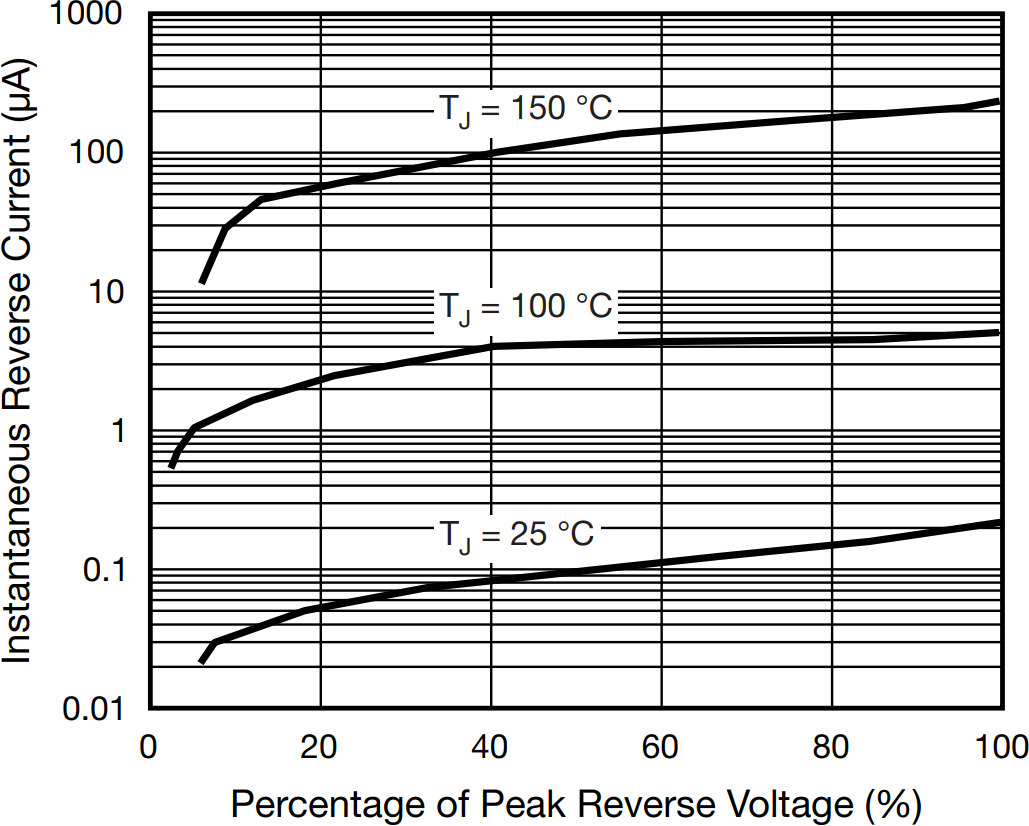
\includegraphics[width=1\textwidth]{images/Curva_Datash_Si_inv.png}
            \caption{Grafico de la curva caracteristica de la hoja de datos.}
            \label{graph.datasheet.Si.inversa}
          \end{minipage}
        \end{figure}

        En la hoja de datos del diodo de silicio \cite{DS0}, se especifica que el voltaje maximo de polarizacion en
        inversa esta en los $1000V$ para el 1N4007. Como se puede ver en la grafica simulada, el punto de ruptura esta
        exactamente al voltaje especificado por el fabricante. Despues de ese voltaje, el diodo entra en region zener,
        y empieza a dejar pasar corriente en inversa, generando una caida de tension especifica. La limitacion de la
        simulacion es que no indica exactamente cuando el diodo va a romperse, por lo que no serviria como una
        aproximacion valida para determinar las condiciones maximas de trabajo.

        Por otro lado, la grafica provista por el fabricante no se parece en nada a la grafica obtenida. Si se observa
        el eje independiente, este indica que dado un porcentaje de corriente de polarizacion inversa, hay una
        corriente de polarizacion inversa asociada, y al mismo tiempo esta corriente depende de la temperatura de la
        juntura. A $25°C$, y al 100\% del voltaje de polarizacion inversa, el diodo deberia dejar pasar aproximadamente
        $200\mu A$ de corriente. Esa corriente no es apreciable en el grafico simulado, pero mas adelante, en la
        comparacion de diodos se va a poder apreciar mejor.

      \subsection{Diodo de Germanio}
        Para corroborar la curva caracteristica en inversa del diodo de germanio, y como esta responde a los cambios de
        voltaje, nuevamente se creo un circuito en el software LTSpice muy basico para probar la polarizacion del diodo
        de germanio.

        El programa, realiza el mismo tipo de barrido que para el diodo de silicio, solamente que ahora el rango es
        desde $-60V$ hasta $10V$.

        Se selecciono nuevamente el diodo 1N60 como diodo de pruebas de germanio y $R_1 = 1K\Omega$. El circuito
        armado en LTSpice se puede ver en figura (\ref{crkt.Ge.inversa}) y se han empleado las directivas mostradas
        en el listado (\ref{list.Ge.inversa}) para la simulacion.

        \begin{figure}[!ht]
          \centering
          \begin{minipage}{0.45\textwidth}
            \begin{circuitikz}[american voltages]
              \draw (0, -1) to [V=$V_1$]                     (0, 3)
                            to [short, -, i<^=$i_D$]         (1, 3)
                            to [R=$R_1$, v<=$V_{R_1}$]       (4, 3)
                            to [short, -]                    (5, 3)
                            to [D=$1N60$, v<=$v_D$]          (5, -1)
                            to [short, -]                    (5, -1)
                            to [short, -]                    (0, -1)
                            ;
            \end{circuitikz}
            \caption{Circuito con diodo de silicio 1N60 en inversa.}
            \label{crkt.Ge.inversa}
          \end{minipage}
          \hfill
          \begin{minipage}{0.45\textwidth}
            \begin{lstlisting}[style=ltspice, caption={Parámetros de simulación LTspice}, label=list.Ge.inversa]
              .dc V1 -60 10 100m
              .model 1N60 D (RS=50.0559 EG=1.11 XTI=3 VJ=0.8 M=0.1 FC=0.5 BV=40 CJO=1.75p IS=1.37773u N=2 TT=100n type=germanium)
            \end{lstlisting}
          \end{minipage}
        \end{figure}

        Los resultados de la simulacion estan presentes en la figura (\ref{graph.simulation.Ge.inversa}).

        \begin{figure}[!ht]
          \centering
          \begin{minipage}{0.45\textwidth}
            \begin{tikzpicture}
              \begin{axis}[
                width=6cm,
                height=5.5cm,
                xlabel={$v_D$ [V]},
                ylabel={$i_D$ [mA]},
                grid=both,
                minor tick num=1,
                scale only axis,
                enlargelimits=false,
                scaled ticks=false,
                extra x ticks={-40},
                extra x tick style={
                  grid style={red, thick, dashed},
                  tick style={red},
                  tick label style={opacity=0}
                 },
                restrict x to domain=-60:11,
                xmin=-60, xmax=10,
              ]
              \addplot[
                color=blue,
                mark=none,
                thick,
              ] table[
                col sep=tab,
                header=true,
                x=V(d1),
                y expr=\thisrow{I(D1)}*1000
              ] {simulations/TP2_2_graph_inv.txt};
              \end{axis}
            \end{tikzpicture}
            \caption{Grafico de la curva caracteristica del simulador.}
            \label{graph.simulation.Ge.inversa}
          \end{minipage}
          \hfill
          \begin{minipage}{0.45\textwidth}
            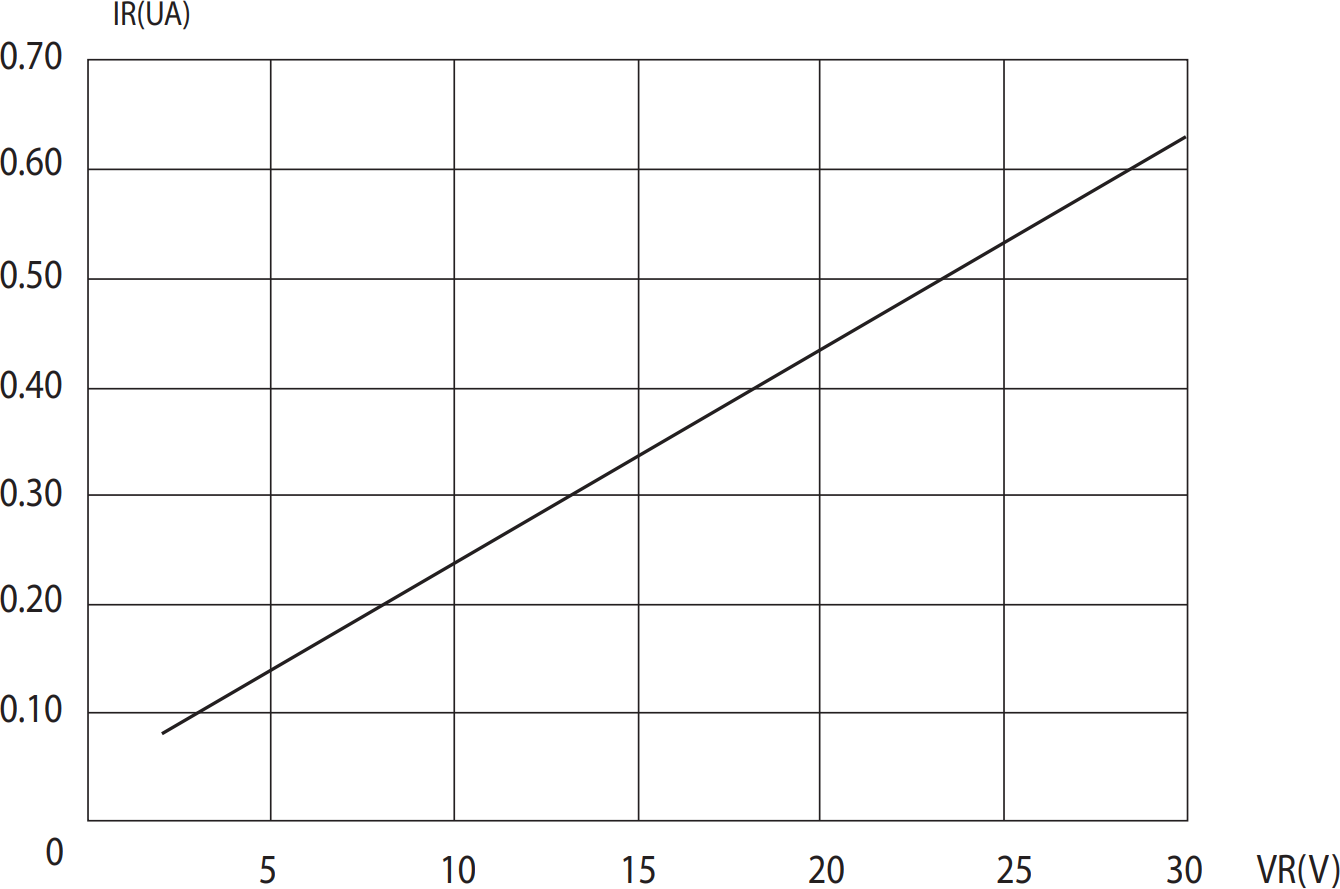
\includegraphics[width=1\textwidth]{images/Curva_Datash_Ge_inv.png}
            \caption{Grafico de la curva caracteristica de la hoja de datos.}
            \label{graph.datasheet.Ge.inversa}
          \end{minipage}
        \end{figure}

        En la hoja de datos del diodo de germanio \cite{DS1}, se especifica que el voltaje maximo de polarizacion en
        inversa esta en los $40V$ para el 1N60. Como se puede ver en la grafica simulada, el punto de ruptura esta
        exactamente al voltaje especificado por el fabricante. Despues de ese voltaje, el diodo entra en region zener,
        y empieza a dejar pasar corriente en inversa, generando una caida de tension especifica. La limitacion de la
        simulacion es que no indica exactamente cuando el diodo va a romperse, por lo que no serviria como una
        aproximacion valida para determinar las condiciones maximas de trabajo.

        Por otro lado, la grafica provista por el fabricante no se parece en nada a la grafica obtenida. La grafica
        indica que a $-30V$ del voltaje de polarizacion inversa, el diodo deberia dejar pasar aproximadamente
        $0.6\mu A$ de corriente. Esa corriente no es apreciable en el grafico simulado, pero mas adelante, en la
        comparacion de diodos se va a poder apreciar mejor.

      \subsection{Comparacion de ambas simulaciones}
        \begin{figure}[!ht]
          \centering
          \begin{minipage}{0.45\textwidth}
            \begin{tikzpicture}
              \begin{axis}[
                width=6cm,
                height=5.5cm,
                xlabel={$v_D$ [V]},
                ylabel={$i_D$ [nA]},
                grid=both,
                minor tick num=1,
                scale only axis,
                enlargelimits=false,
                scaled ticks=false,
                extra x ticks={-1000},
                extra x tick style={
                  grid style={red, thick, dashed},
                  tick style={red},
                  tick label style={opacity=0}
                 },
                restrict x to domain=-1005:-995,
                restrict y to domain=-100:100,
                ymin=-2, ymax=0.5,
                xmin=-1003, xmax=-997,
              ]
              \addplot[
                color=blue,
                mark=none,
                thick,
              ] table[
                col sep=tab,
                header=true,
                x=V(d1),
                y expr=\thisrow{I(D1)}*1000000000
              ] {simulations/TP2_1_graph_inv.txt};
                \addlegendentry{Si}
              \end{axis}
            \end{tikzpicture}
          \end{minipage}
          \hfill
          \begin{minipage}{0.45\textwidth}
            \begin{tikzpicture}
              \begin{axis}[
                width=6cm,
                height=5.5cm,
                xlabel={$v_D$ [V]},
                ylabel={$i_D$ [$\mu A$]},
                grid=both,
                minor tick num=1,
                scale only axis,
                enlargelimits=false,
                scaled ticks=false,
                extra x ticks={-40},
                extra x tick style={
                  grid style={red, thick, dashed},
                  tick style={red},
                  tick label style={opacity=0}
                 },
                restrict x to domain=-45:-35,
                restrict y to domain=-100:100,
                ymin=-5, ymax=2,
                xmin=-43, xmax=-37,
              ]
              \addplot[
                color=blue,
                mark=none,
                thick,
              ] table[
                col sep=tab,
                header=true,
                x=V(d1),
                y expr=\thisrow{I(D1)}*1000000
              ] {simulations/TP2_2_graph_inv.txt};
              \addlegendentry{Ge}
              \end{axis}
            \end{tikzpicture}
          \end{minipage}
          \caption{Grafico de las curvas caracteristicas simuladas de los diodos de Silicio y Germanio utilizados.}
          \label{graph.simulation.comparativa.inversa}
        \end{figure}

        Se puede apreciar las diferencias principales de los diodos de germanio contra los diodos de silicio con mucha
        claridad. El diodo de germanio, a pesar de tener una tension de polarizacion baja comparada con el diodo de
        silicio, tiene una corriente de fuga 1000 veces mas grande que la corriente de fuga del silicio. Esto puede
        significar un problema, ya que puede producir corrientes indeseadas en circuitos donde un diodo de silicio
        practicamente no permitiria el paso de la misma.

        Como el diodo se lo considera idealmente como un elemento que deja pasar la corriente para un lado y no para
        el otro, el diodo de silicio se comporta mejor como ese componente que el diodo de germanio.


  \chapter{Curva caracteristica del Diodo: Laboratorio}
    Se pide poner en practica y corroborar los datos conseguidos en el simulador y armar el mismo circuito
    propuesto y anotar los valores conseguidos. Para ello, se armaron los circuitos correspondientes y se tomo nota de
    los valores de caida de tension del diodo, desde 0v hasta 5v, tomando mas muestras cerca del codo de conduccion
    para el diodo de silicio y germanio.

    Como no disponemos de equipamento con la presicion necesaria para medir la corriente de polarizacion inversa, se
    omitio la prueba. Ademas, en el caso del diodo de silicio, es peligroso intentar hacer la prueba de polarizacion
    inversa debido a que el voltaje es excesivamente elevado.

    \section{Diodo de Silicio}
      Se armo el circuito de la figura (\ref{crkt.Si.directa}) para realizar las pruebas.
      \begin{figure}[!ht]
        \centering
        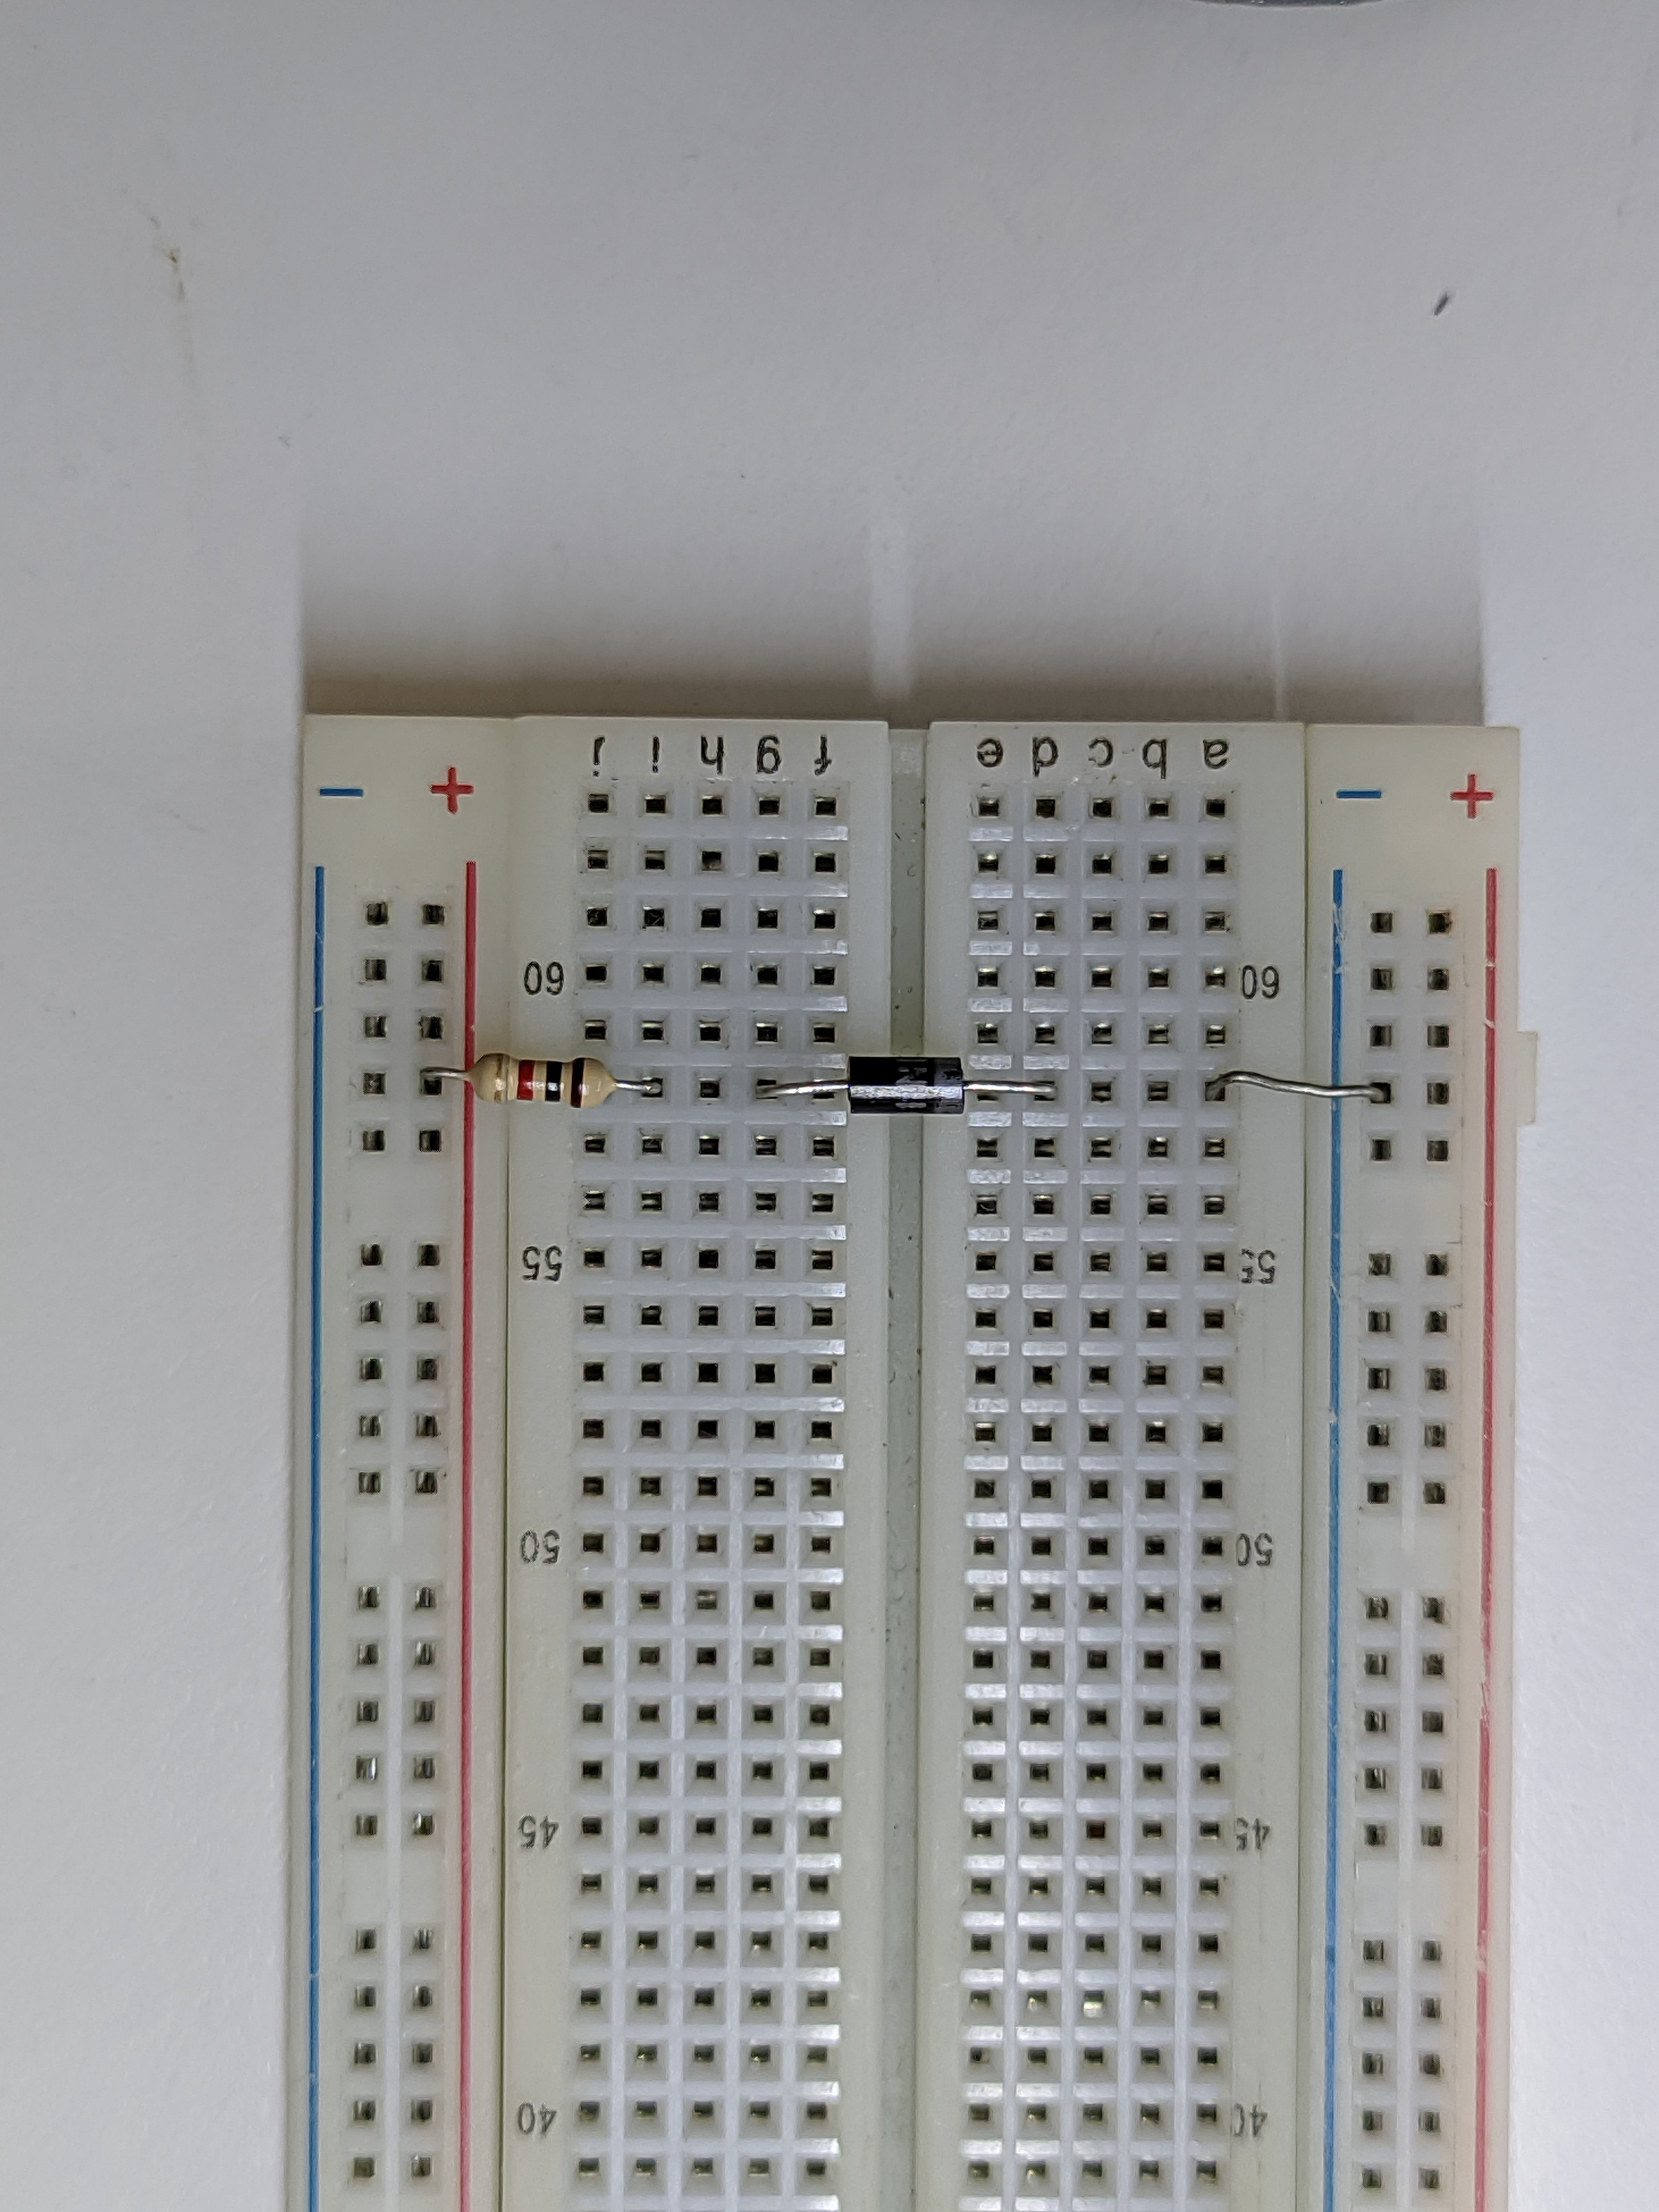
\includegraphics[angle=180, width=.8\textwidth]{pictures/prot_crkt-1.jpg}
        \caption{Circuito de prueba con el 1N4007}
        \label{crkt.Si.prot}
      \end{figure}

      Para poder realizar las mediciones de corriente, tension de entrada, y caida de tension del diodo, se utilizaron
      tres multimetros en conjunto, con sus puntas dispuestas como se ve en las figuras (\ref{crkt.Si.mult.curr}),
      (\ref{crkt.Si.mult.vi}) y (\ref{crkt.Si.mult.vd}).
      \begin{figure}[H]
        \centering
        \begin{minipage}{0.3\textwidth}
          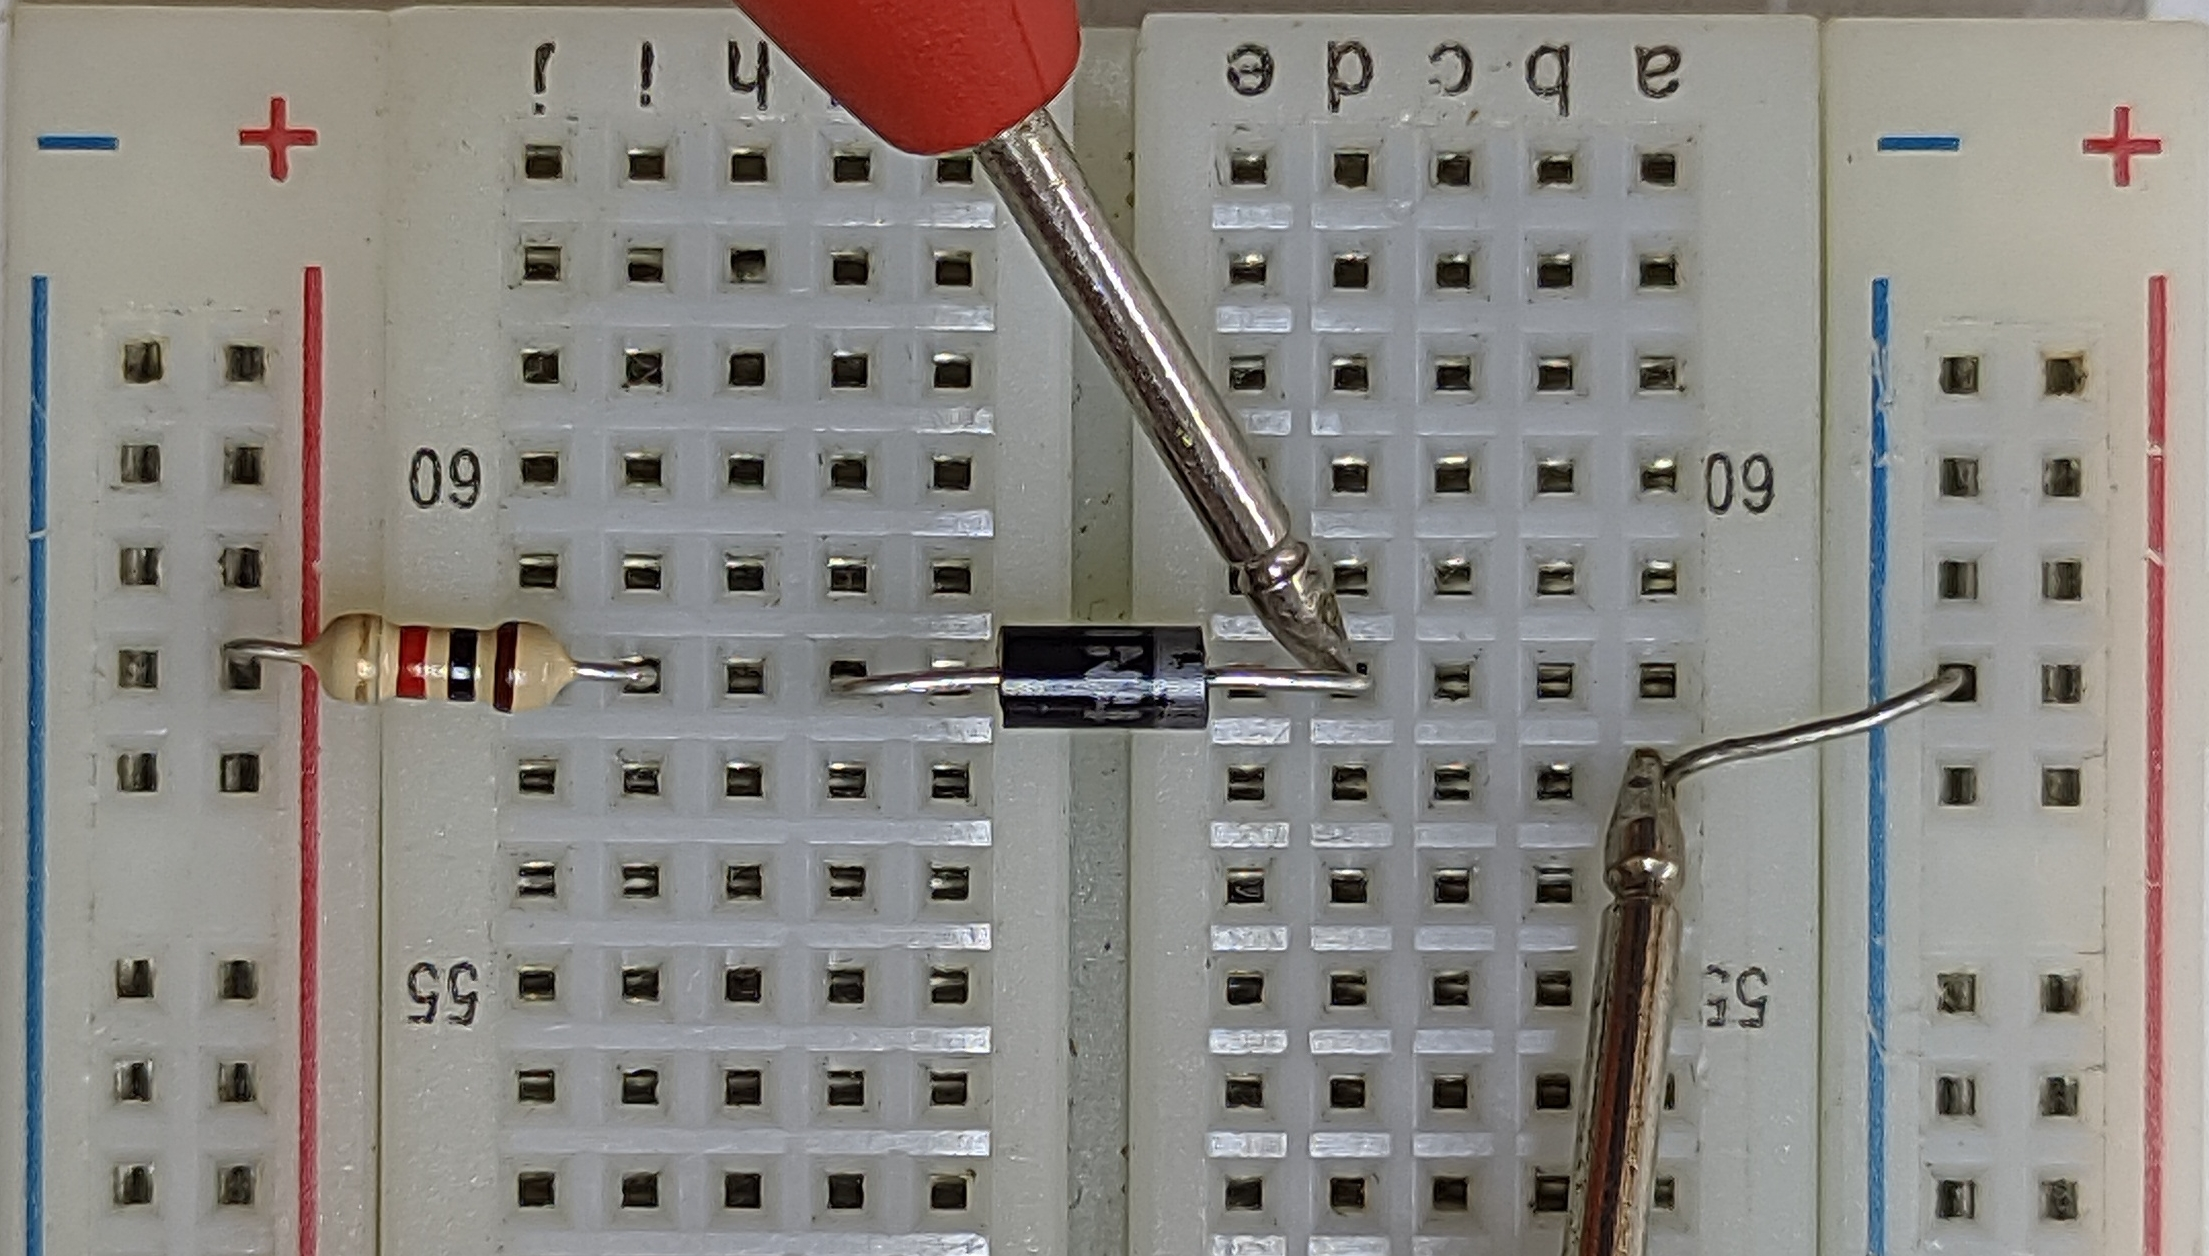
\includegraphics[angle=180, width=1\textwidth]{pictures/prot_crkt-1_curr.jpg}
          \caption{Medicion de corriente del circuito.}
          \label{crkt.Si.mult.curr}
        \end{minipage}
        \begin{minipage}{0.3\textwidth}
          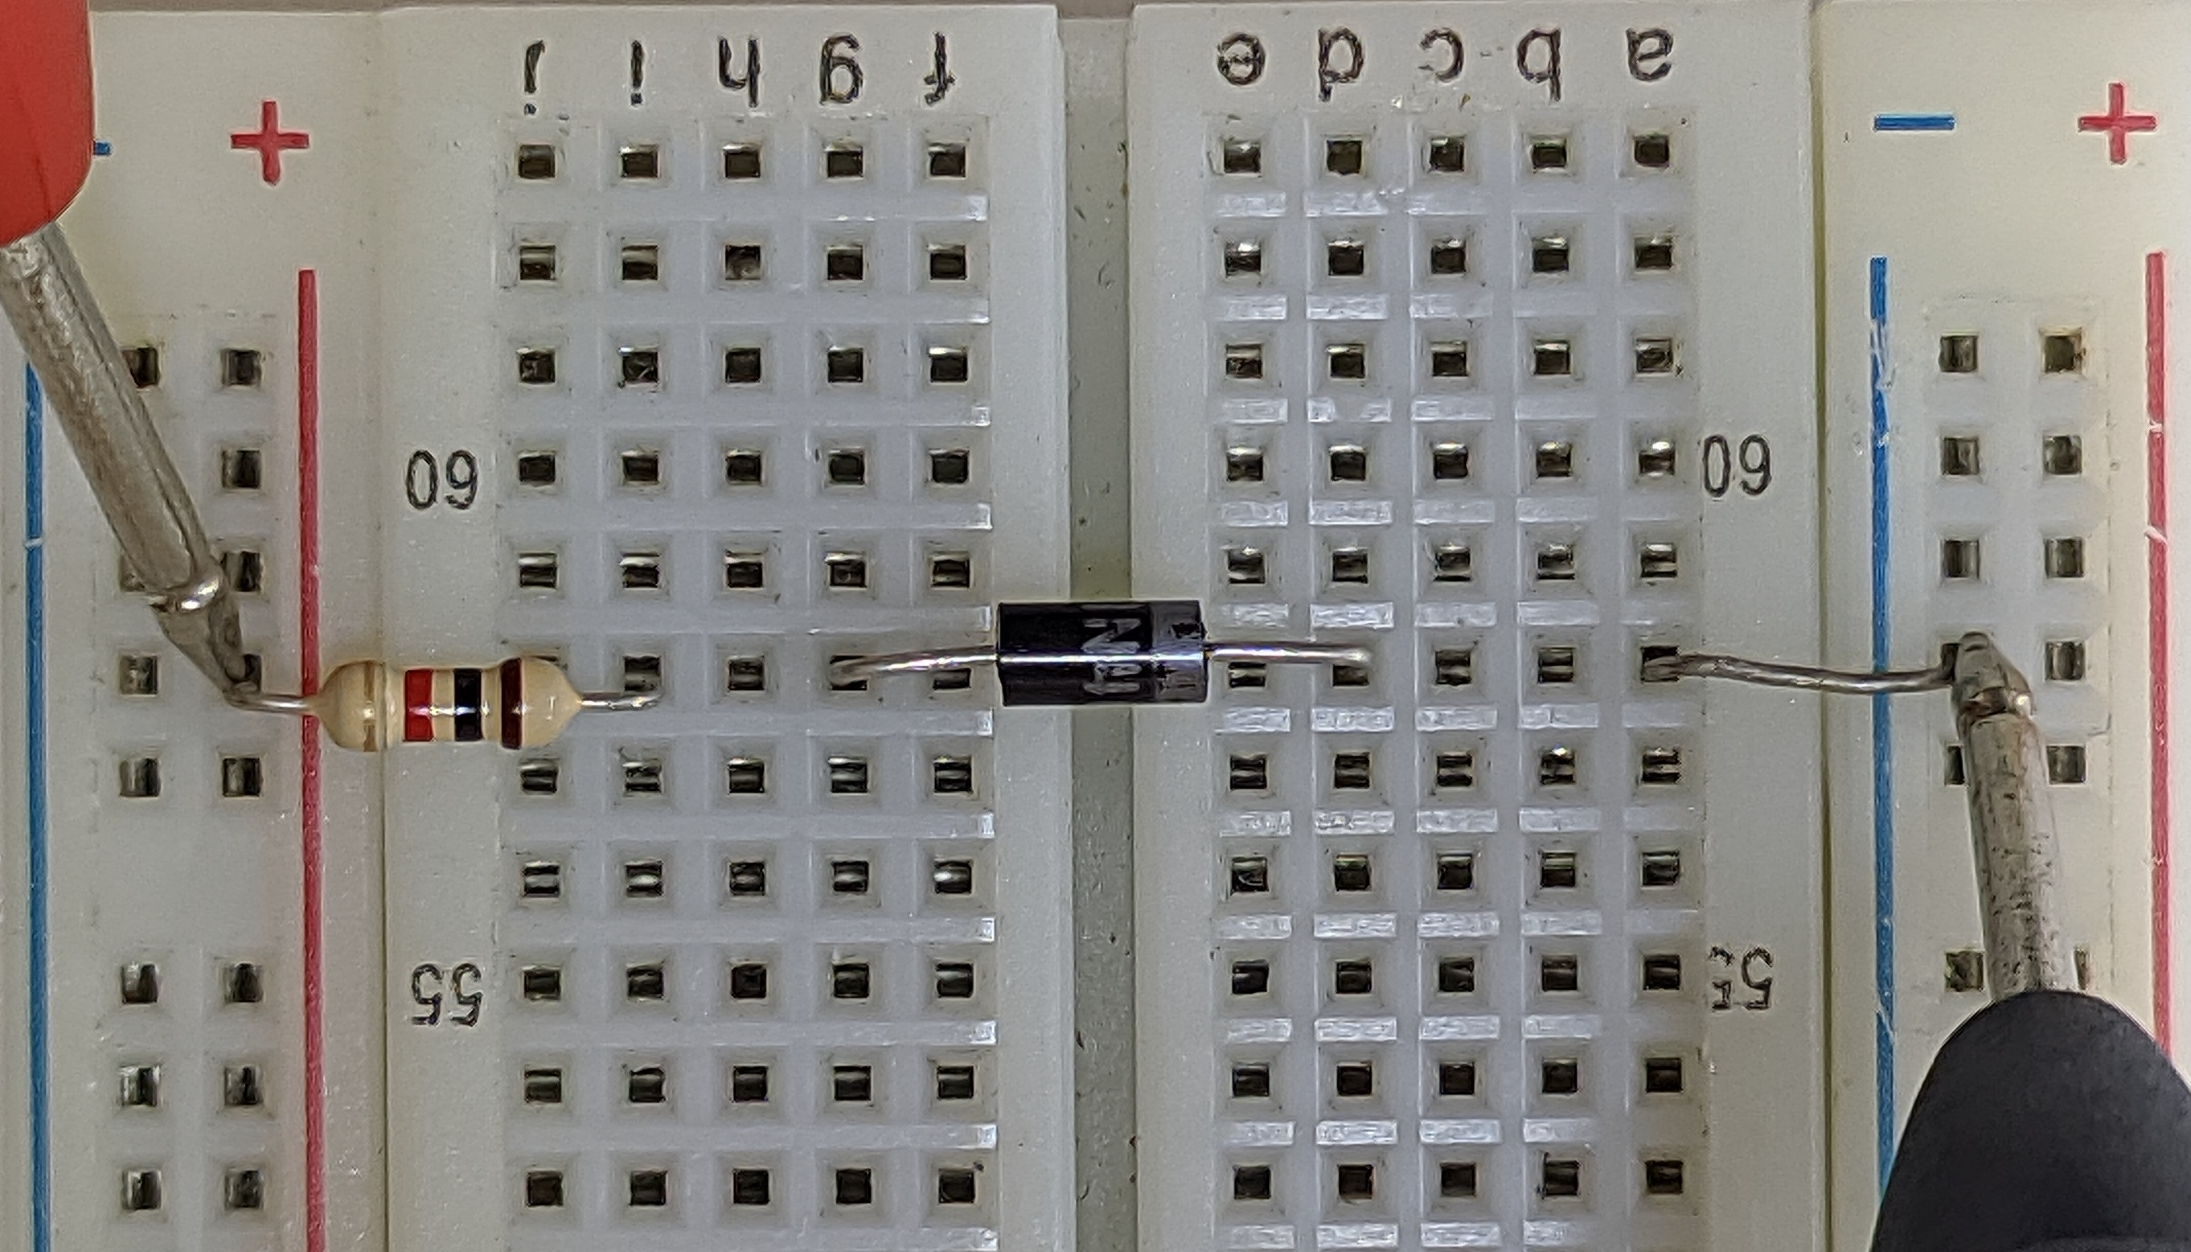
\includegraphics[angle=180, width=1\textwidth]{pictures/prot_crkt-1_vi.jpg}
          \caption{Medicion de tension de la fuente.}
          \label{crkt.Si.mult.vi}
        \end{minipage}
        \begin{minipage}{0.3\textwidth}
          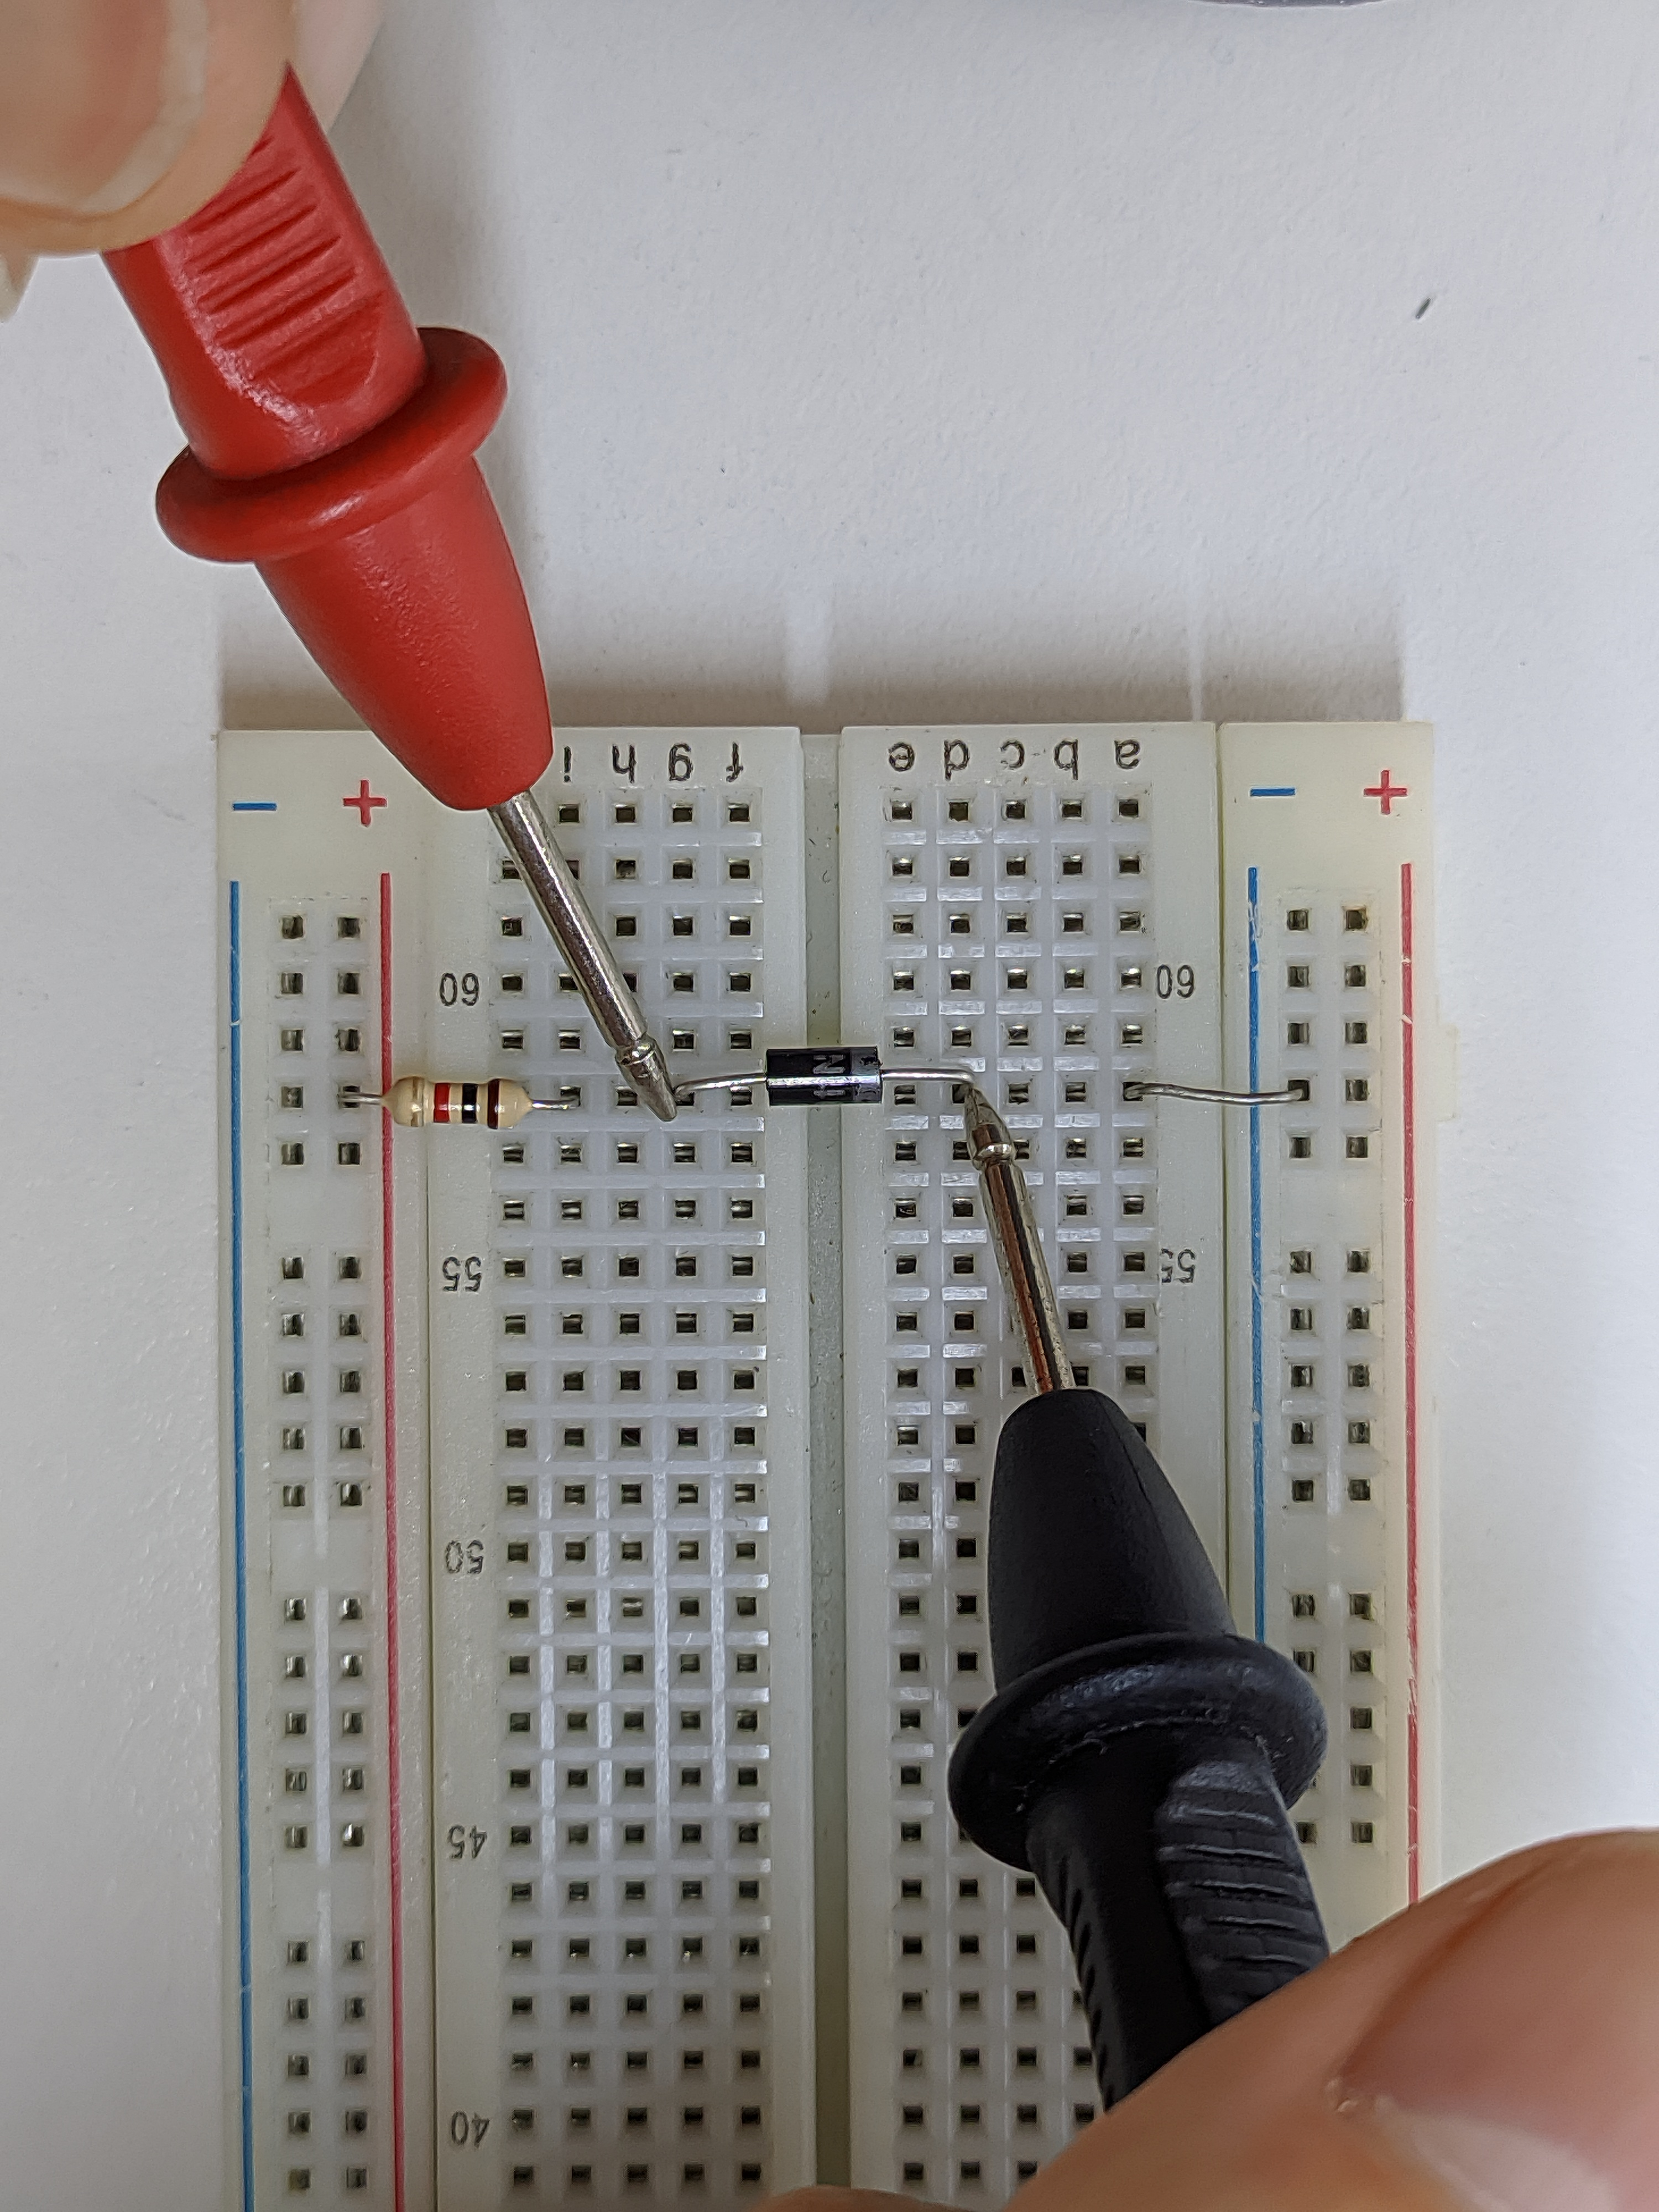
\includegraphics[angle=180, width=1\textwidth]{pictures/prot_crkt-1_vd.jpg}
          \caption{Medicion de caida de tension del diodo.}
          \label{crkt.Si.mult.vd}
        \end{minipage}
      \end{figure}

      Con el circuito de la figura (\ref{crkt.Si.prot}), y los tres multimetros midiendo al mismo tiempo, procedimos a
      hacer las variaciones de voltaje de entrada y tomar muestras de todas los valores.

      \begin{figure}[!ht]
        \centering
        \begin{minipage}{0.25\textwidth}
          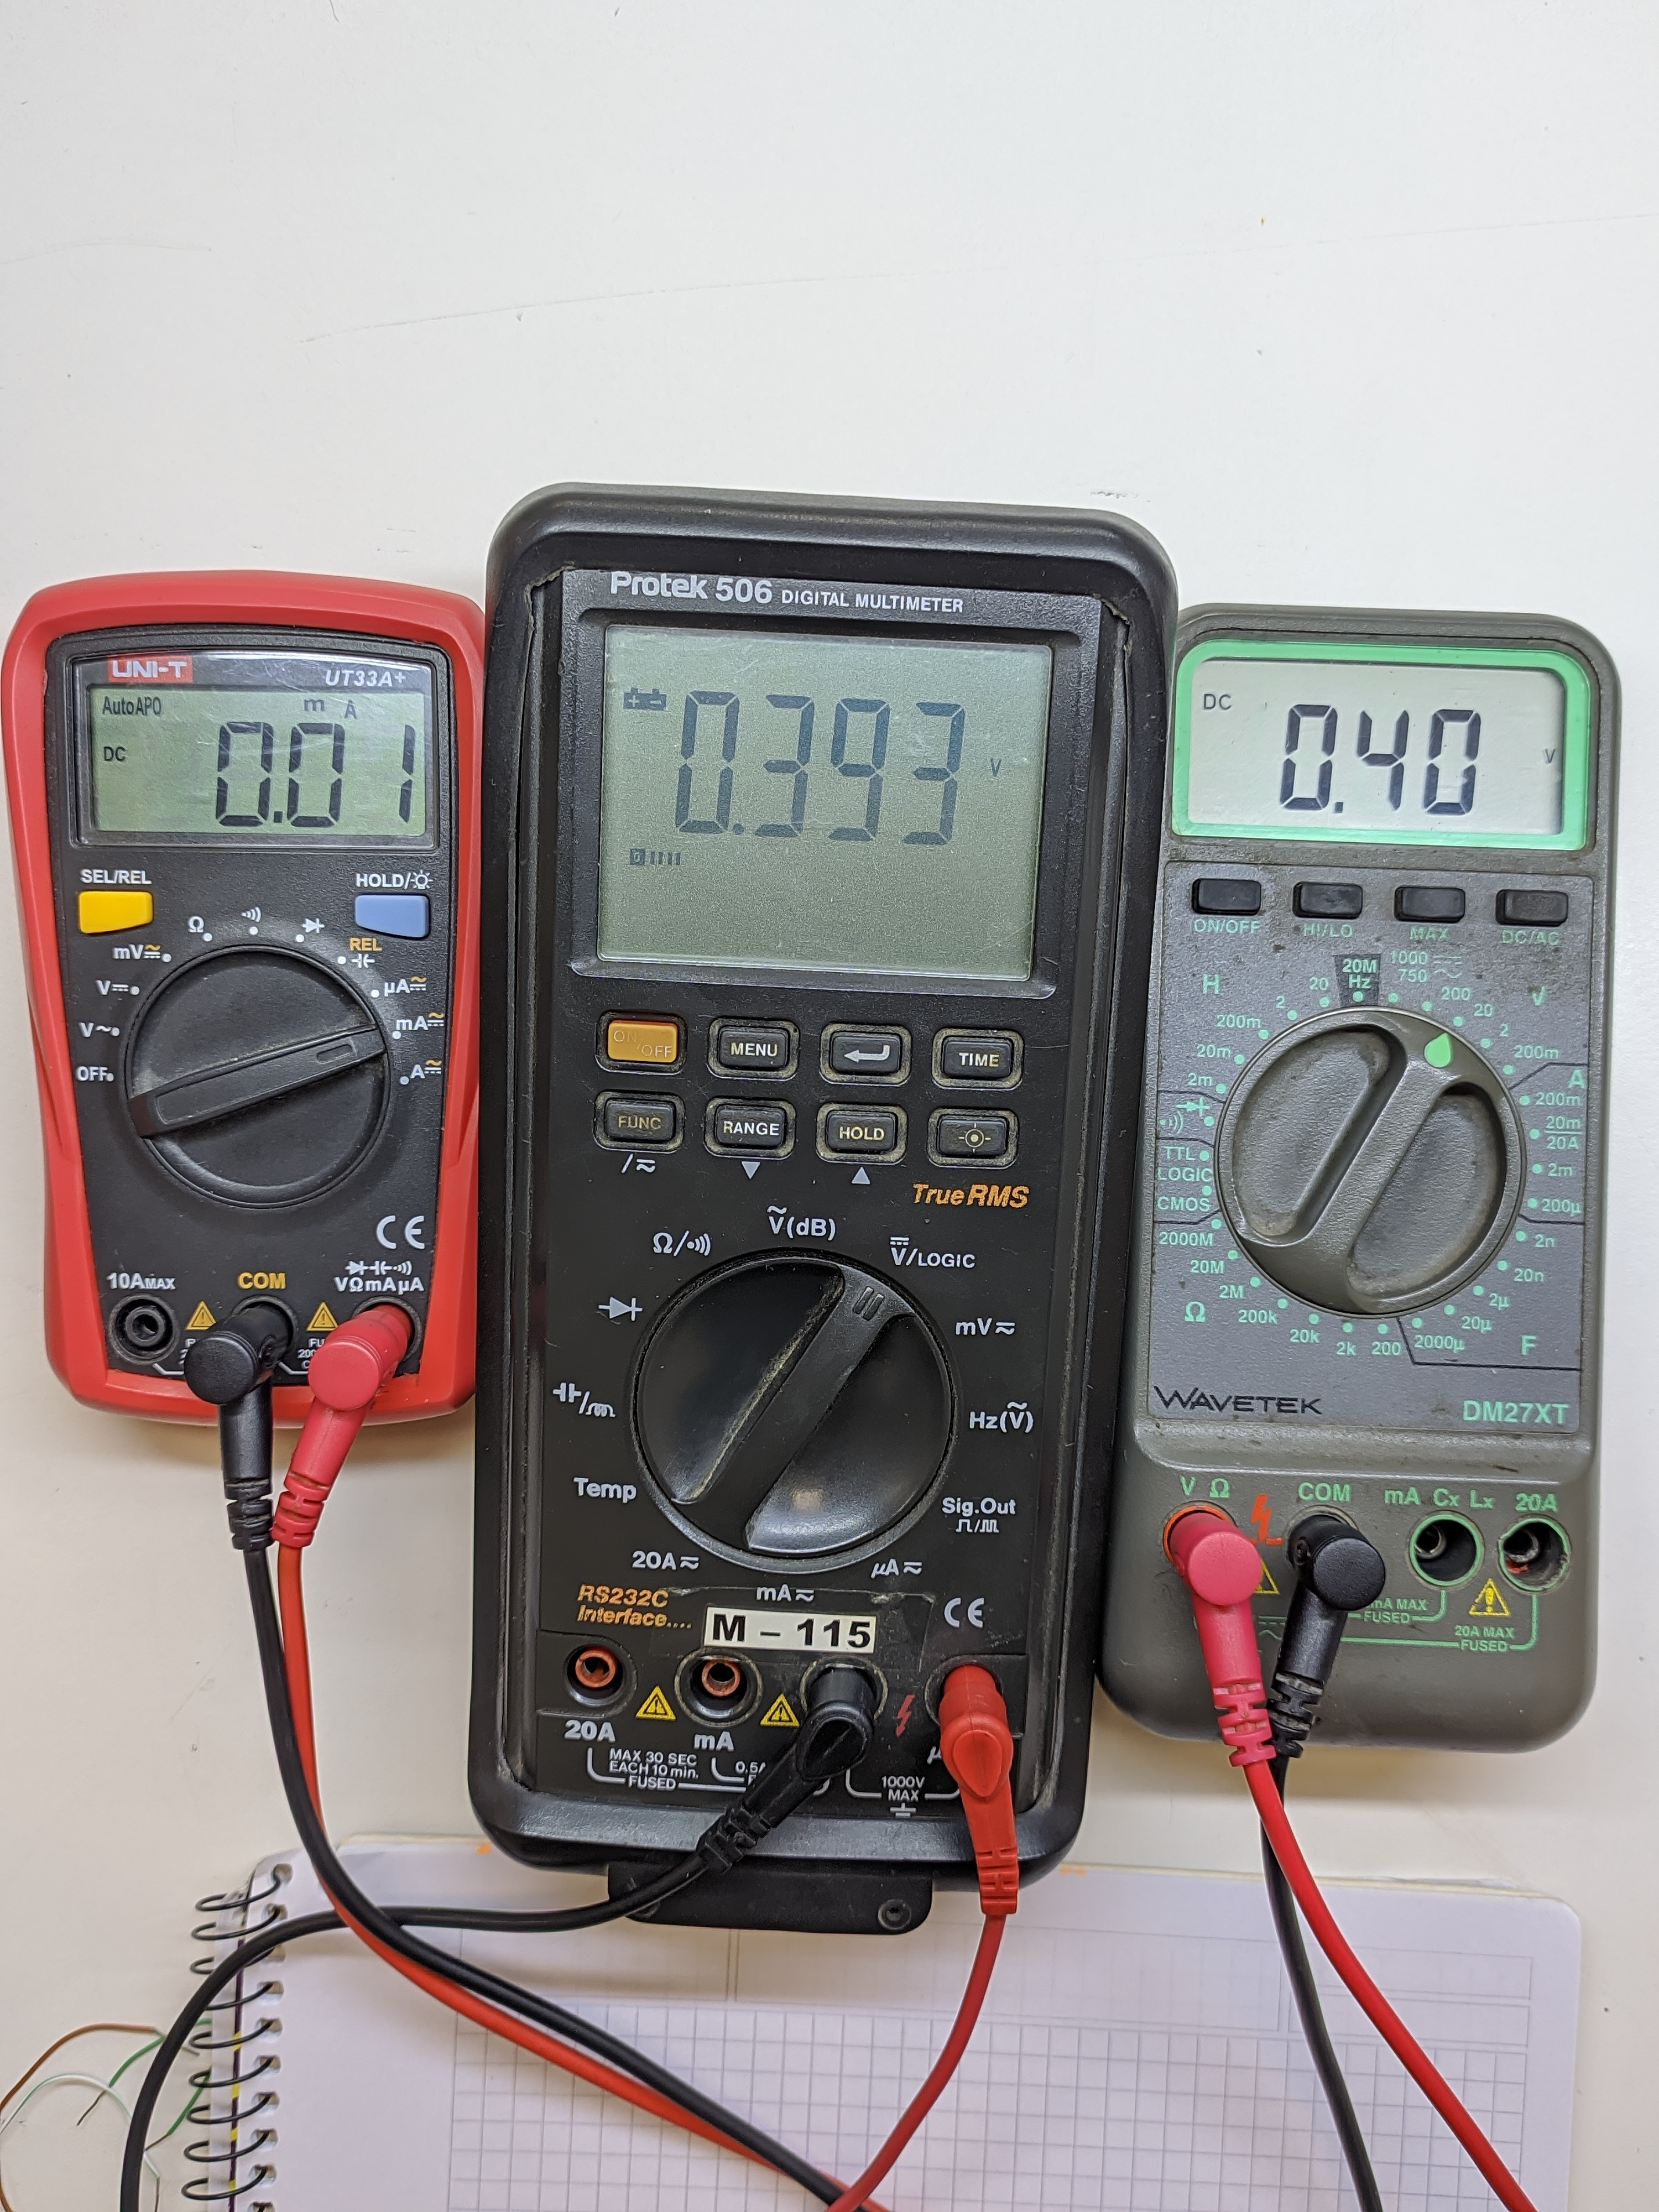
\includegraphics[width=1\textwidth]{pictures/mult_crkt-1_03.jpg}
        \end{minipage}
        \begin{minipage}{0.25\textwidth}
          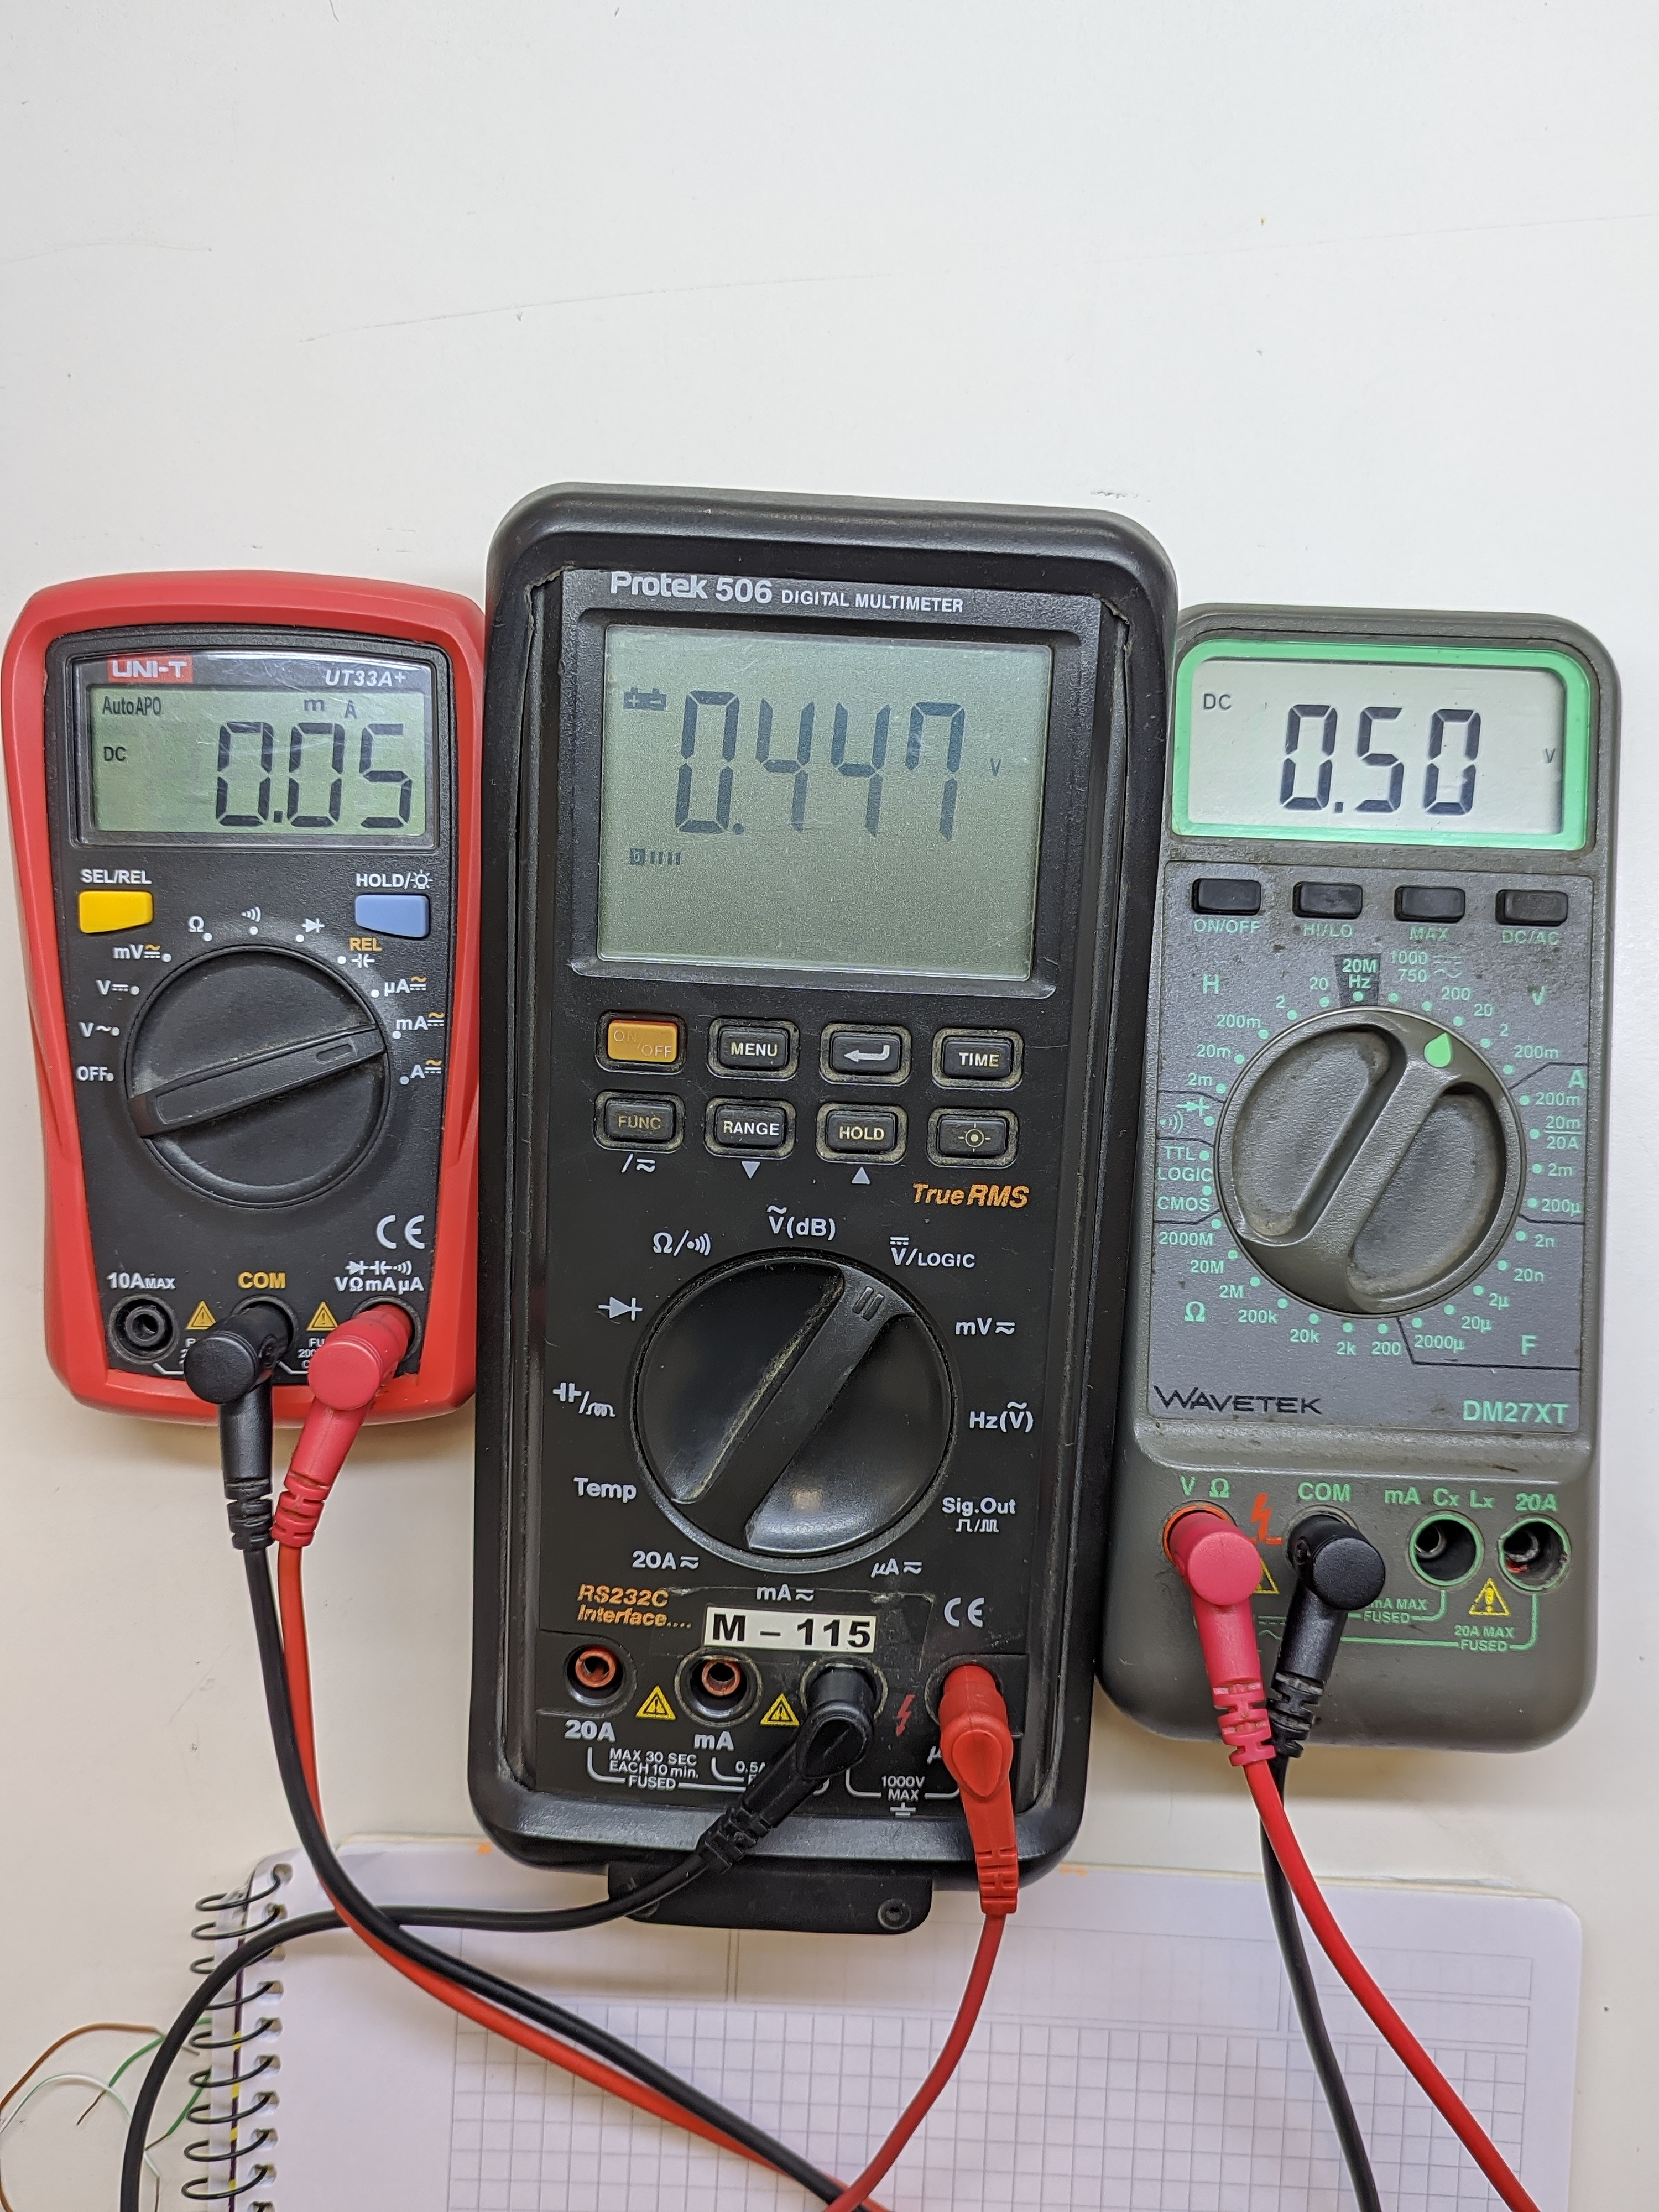
\includegraphics[width=1\textwidth]{pictures/mult_crkt-1_05.jpg}
        \end{minipage}
        \begin{minipage}{0.25\textwidth}
          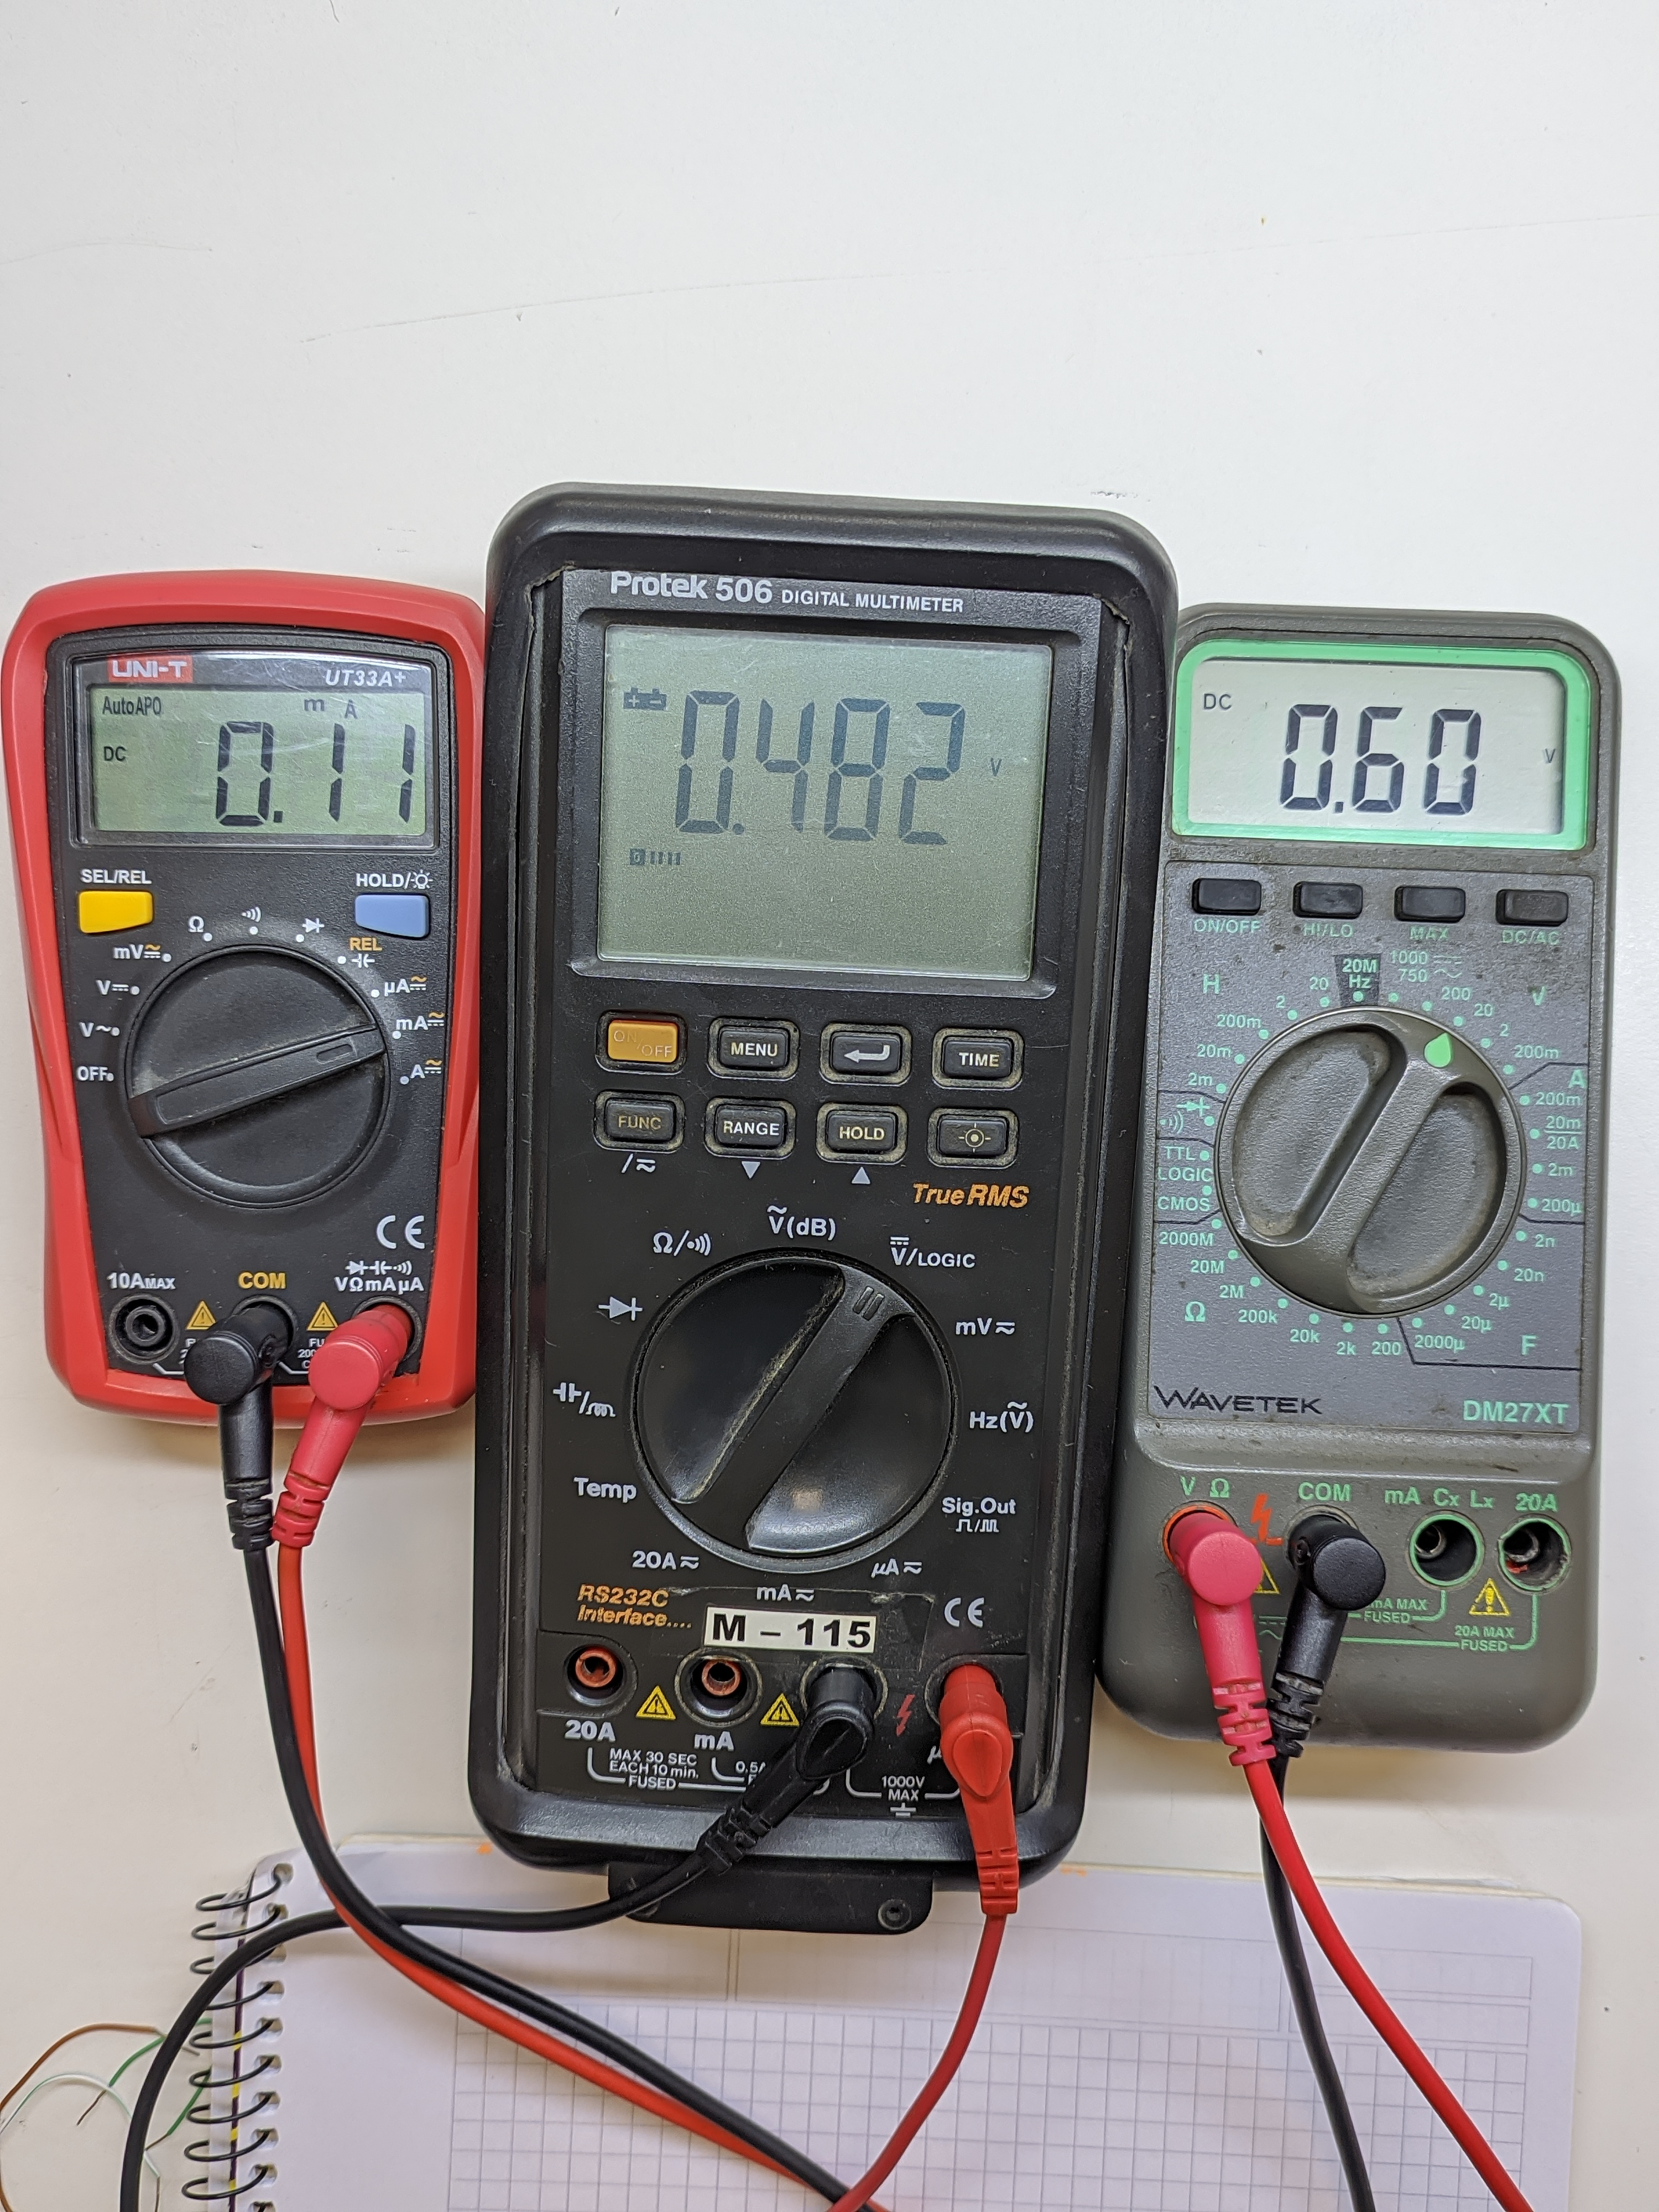
\includegraphics[width=1\textwidth]{pictures/mult_crkt-1_07.jpg}
        \end{minipage}
        \caption{Algunas fotos de las mediciones de los tres multimetros. El de la izquierda mide corriente en mA, el
        del medio mide la caida de tension del diodo y el de la derecha mide la entrada de la fuente}
      \end{figure}

      \begin{table}[H]
        \resizebox{\textwidth}{!}{\begin{tabular}{|c|c|c|c|c|c|c|c|c|c|c|c|c|}
          \hline
          $V_{in}$ & 100mV & 280mV & 400mV & 450mV & 500mV & 550mV & 600mV & 640mV & 700mV & 1V & 3V & 5V\\
          \hline
          $I_t$    & 0A & 0A & 0.01mA & 0.02mA & 0.05mA & 0.07mA & 0.11mA & 0.15mA & 0.2mA & 0.46mA & 2.36mA & 4.33mA\\
          \hline
          $v_D$    & 100mV & 280mV & 390mV & 420mV & 440mV & 460mV & 480mV & 490mV & 500mV & 550mV & 640mV & 680mV\\
          \hline
        \end{tabular}}
        \caption{Tabla de valores medidos del diodo de silicio.}
        \label{table.Si}
      \end{table}

      Con los datos de la tabla (\ref{table.Si}), podemos hacer una curva y compararla con la curva simulada.
      \begin{figure}[!ht]
        \centering
        \begin{tikzpicture}
          \begin{axis}[
            width=14cm,
            height=7cm,
            xlabel={$v_D$ [V]},
            ylabel={$i_D$ [mA]},
            grid=both,
            minor tick num=1,
            scale only axis,
            enlargelimits=false,
            scaled ticks=false,
            restrict x to domain=-0.2:1,
          ]
          \addplot[
            color=blue,
            mark=none,
            thick,
          ] table[
            col sep=tab,
            header=true,
            x=V(d1),
            y expr=\thisrow{I(D1)}*1000
          ] {simulations/TP2_1_graph.txt};
          \addlegendentry{Simulada}
          \addplot[
            color=red,
            mark=none,
            thick,
          ] coordinates {(.1, 0)(.28, 0)(.39, 0.01)(.42, 0.02)(.44, 0.05)(.46, 0.07)(.48, 0.11)(.49, 0.15)(.5, 0.2)(0.55, 0.46)(0.64, 2.36)(0.68, 4.33)};
          \addlegendentry{Medida}
          \end{axis}
        \end{tikzpicture}
        \caption{Grafico de la curva caracteristica simulada y la medida experimentalmente del diodo de Silicio.}
        \label{graph.comparativa.Si}
      \end{figure}

      Como se puede ver en la figura (\ref{graph.comparativa.Si}), la curva medida se acerca bastante a la curva
      simulada, por lo que podemos afirmar que para la polarizacion en directa, el modelo de simulacion es lo
      suficientemente preciso. Es muy posible que la pequeña variacion de la corriente se deba por alguna resistencia
      de contacto, ya sea en el circuito o en los cables del multimetro.

    \section{Diodo de Germanio}
      Se armo el circuito de la figura (\ref{crkt.Ge.directa}) para realizar las pruebas.
      \begin{figure}[H]
        \centering
        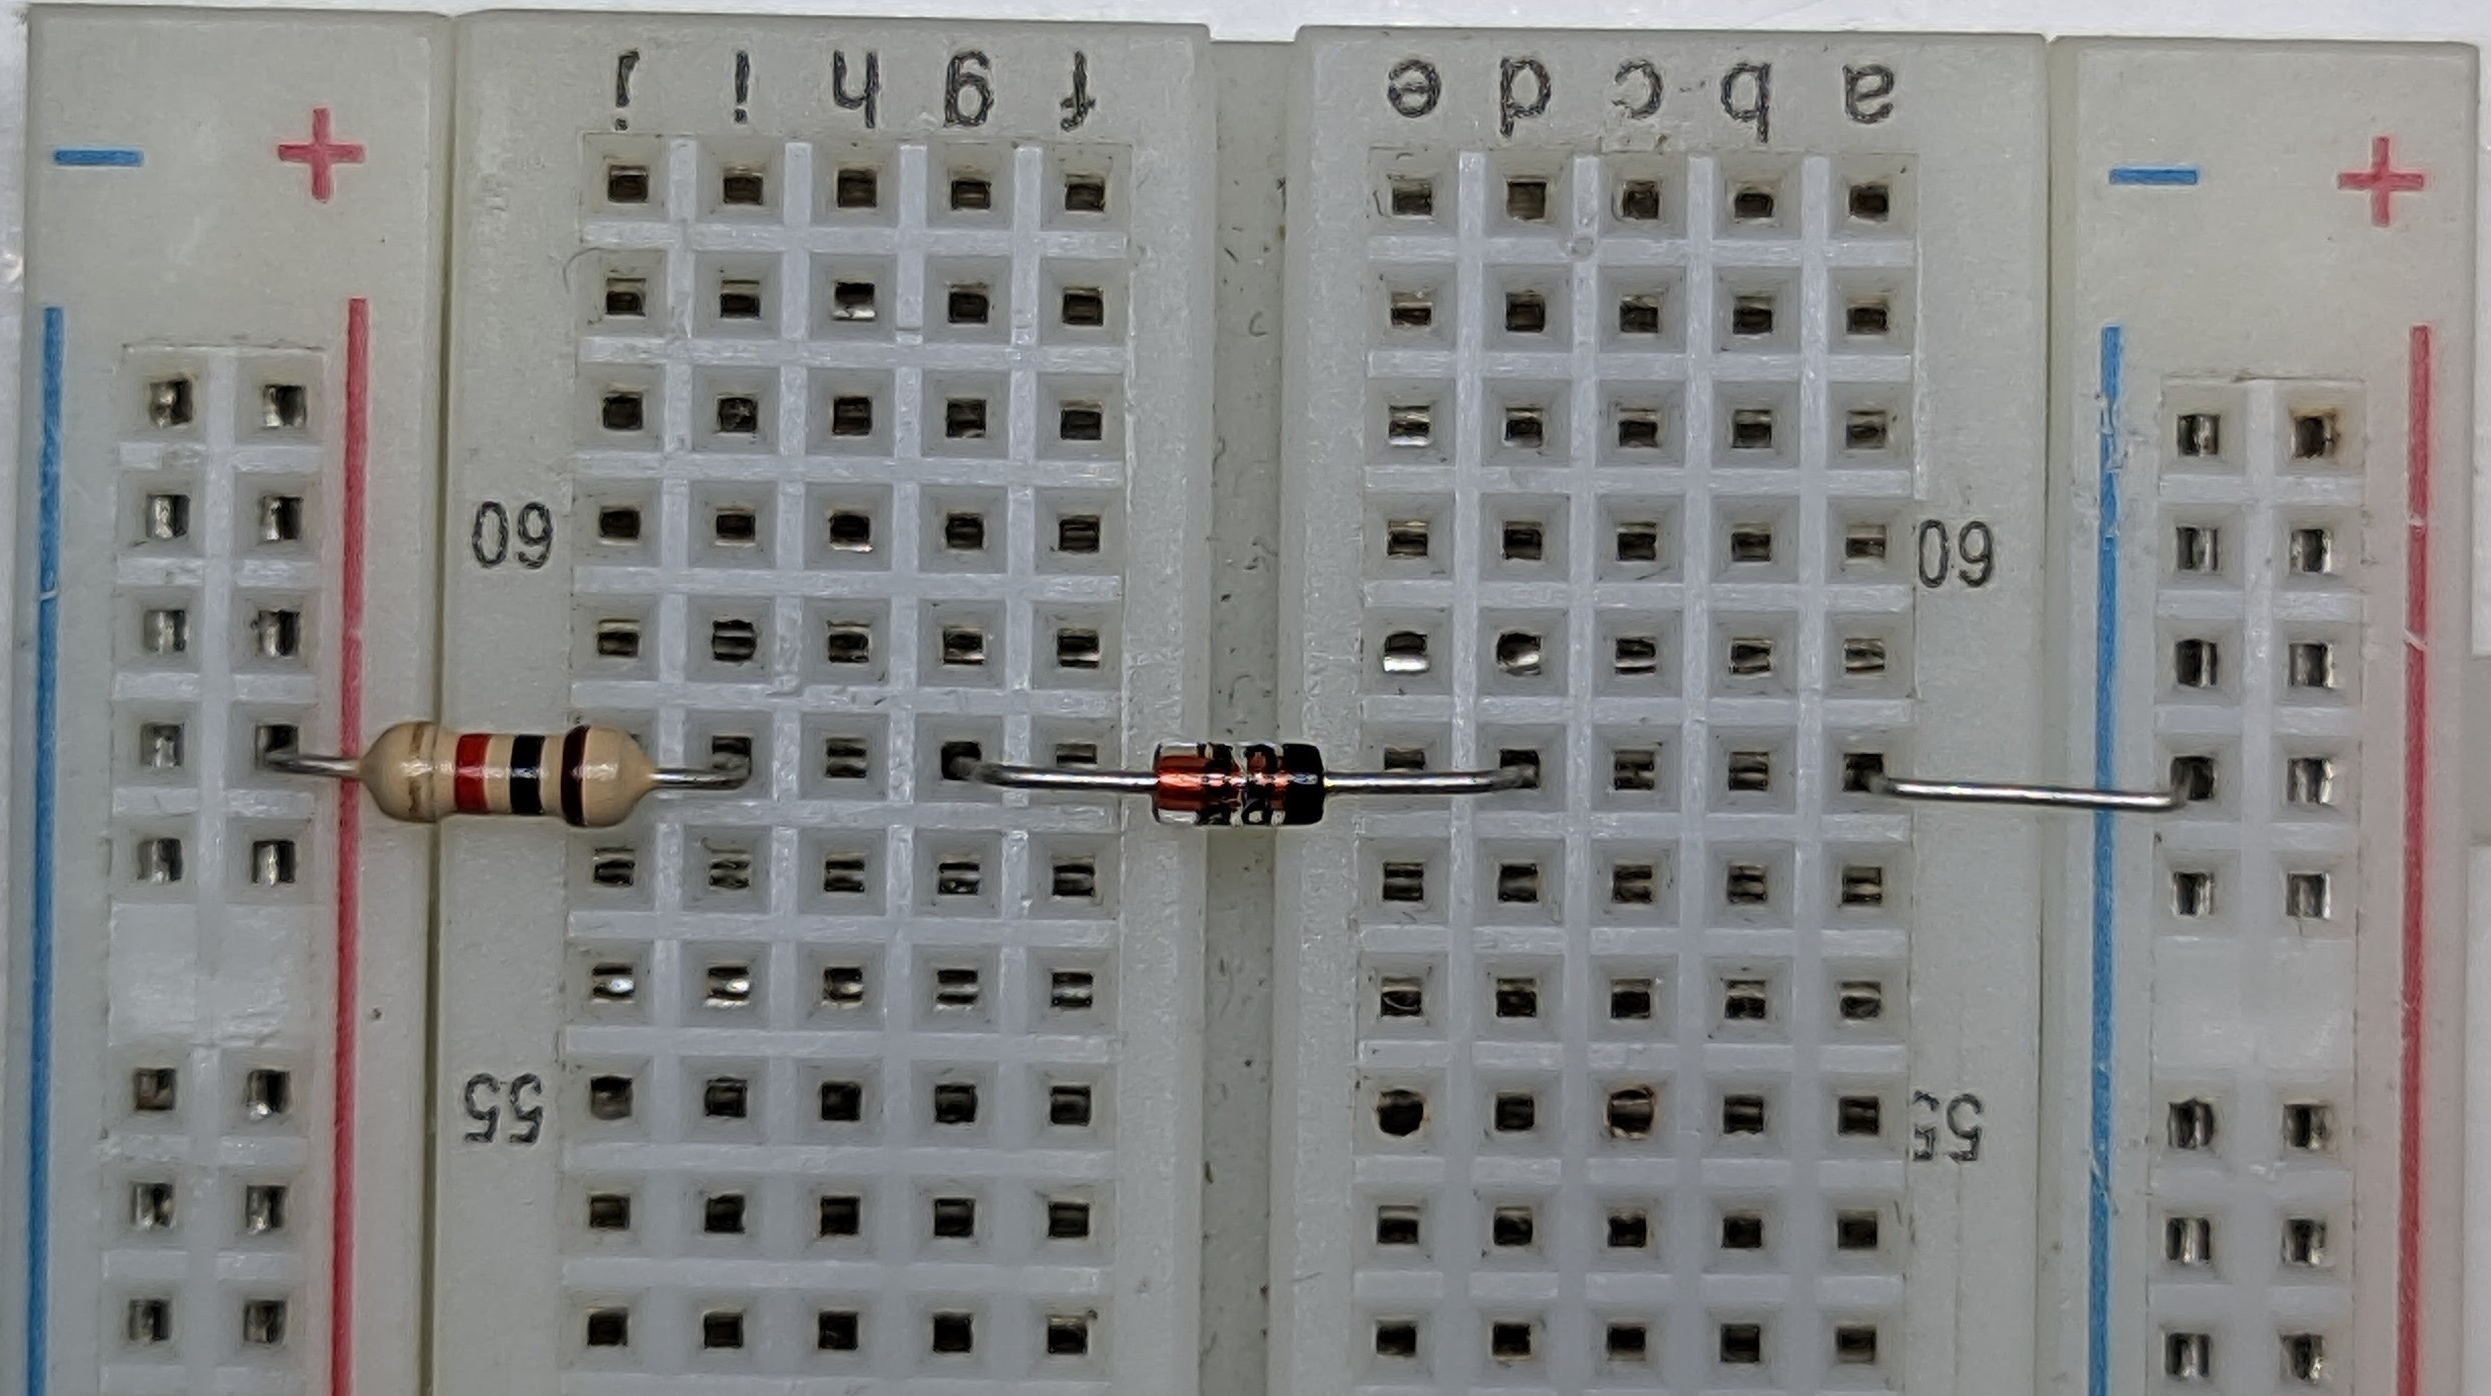
\includegraphics[angle=180, width=.8\textwidth]{pictures/prot_crkt-2.jpg}
        \caption{Circuito de prueba con el 1N60}
        \label{crkt.Ge.prot}
      \end{figure}

      Para poder realizar las mediciones de corriente, tension de entrada, y caida de tension del diodo, se utilizaron
      tres multimetros en conjunto, con sus puntas dispuestas como se ve en las figuras (\ref{crkt.Ge.mult.curr}),
      (\ref{crkt.Ge.mult.vi}) y (\ref{crkt.Ge.mult.vd}).
      \begin{figure}[H]
        \centering
        \begin{minipage}{0.3\textwidth}
          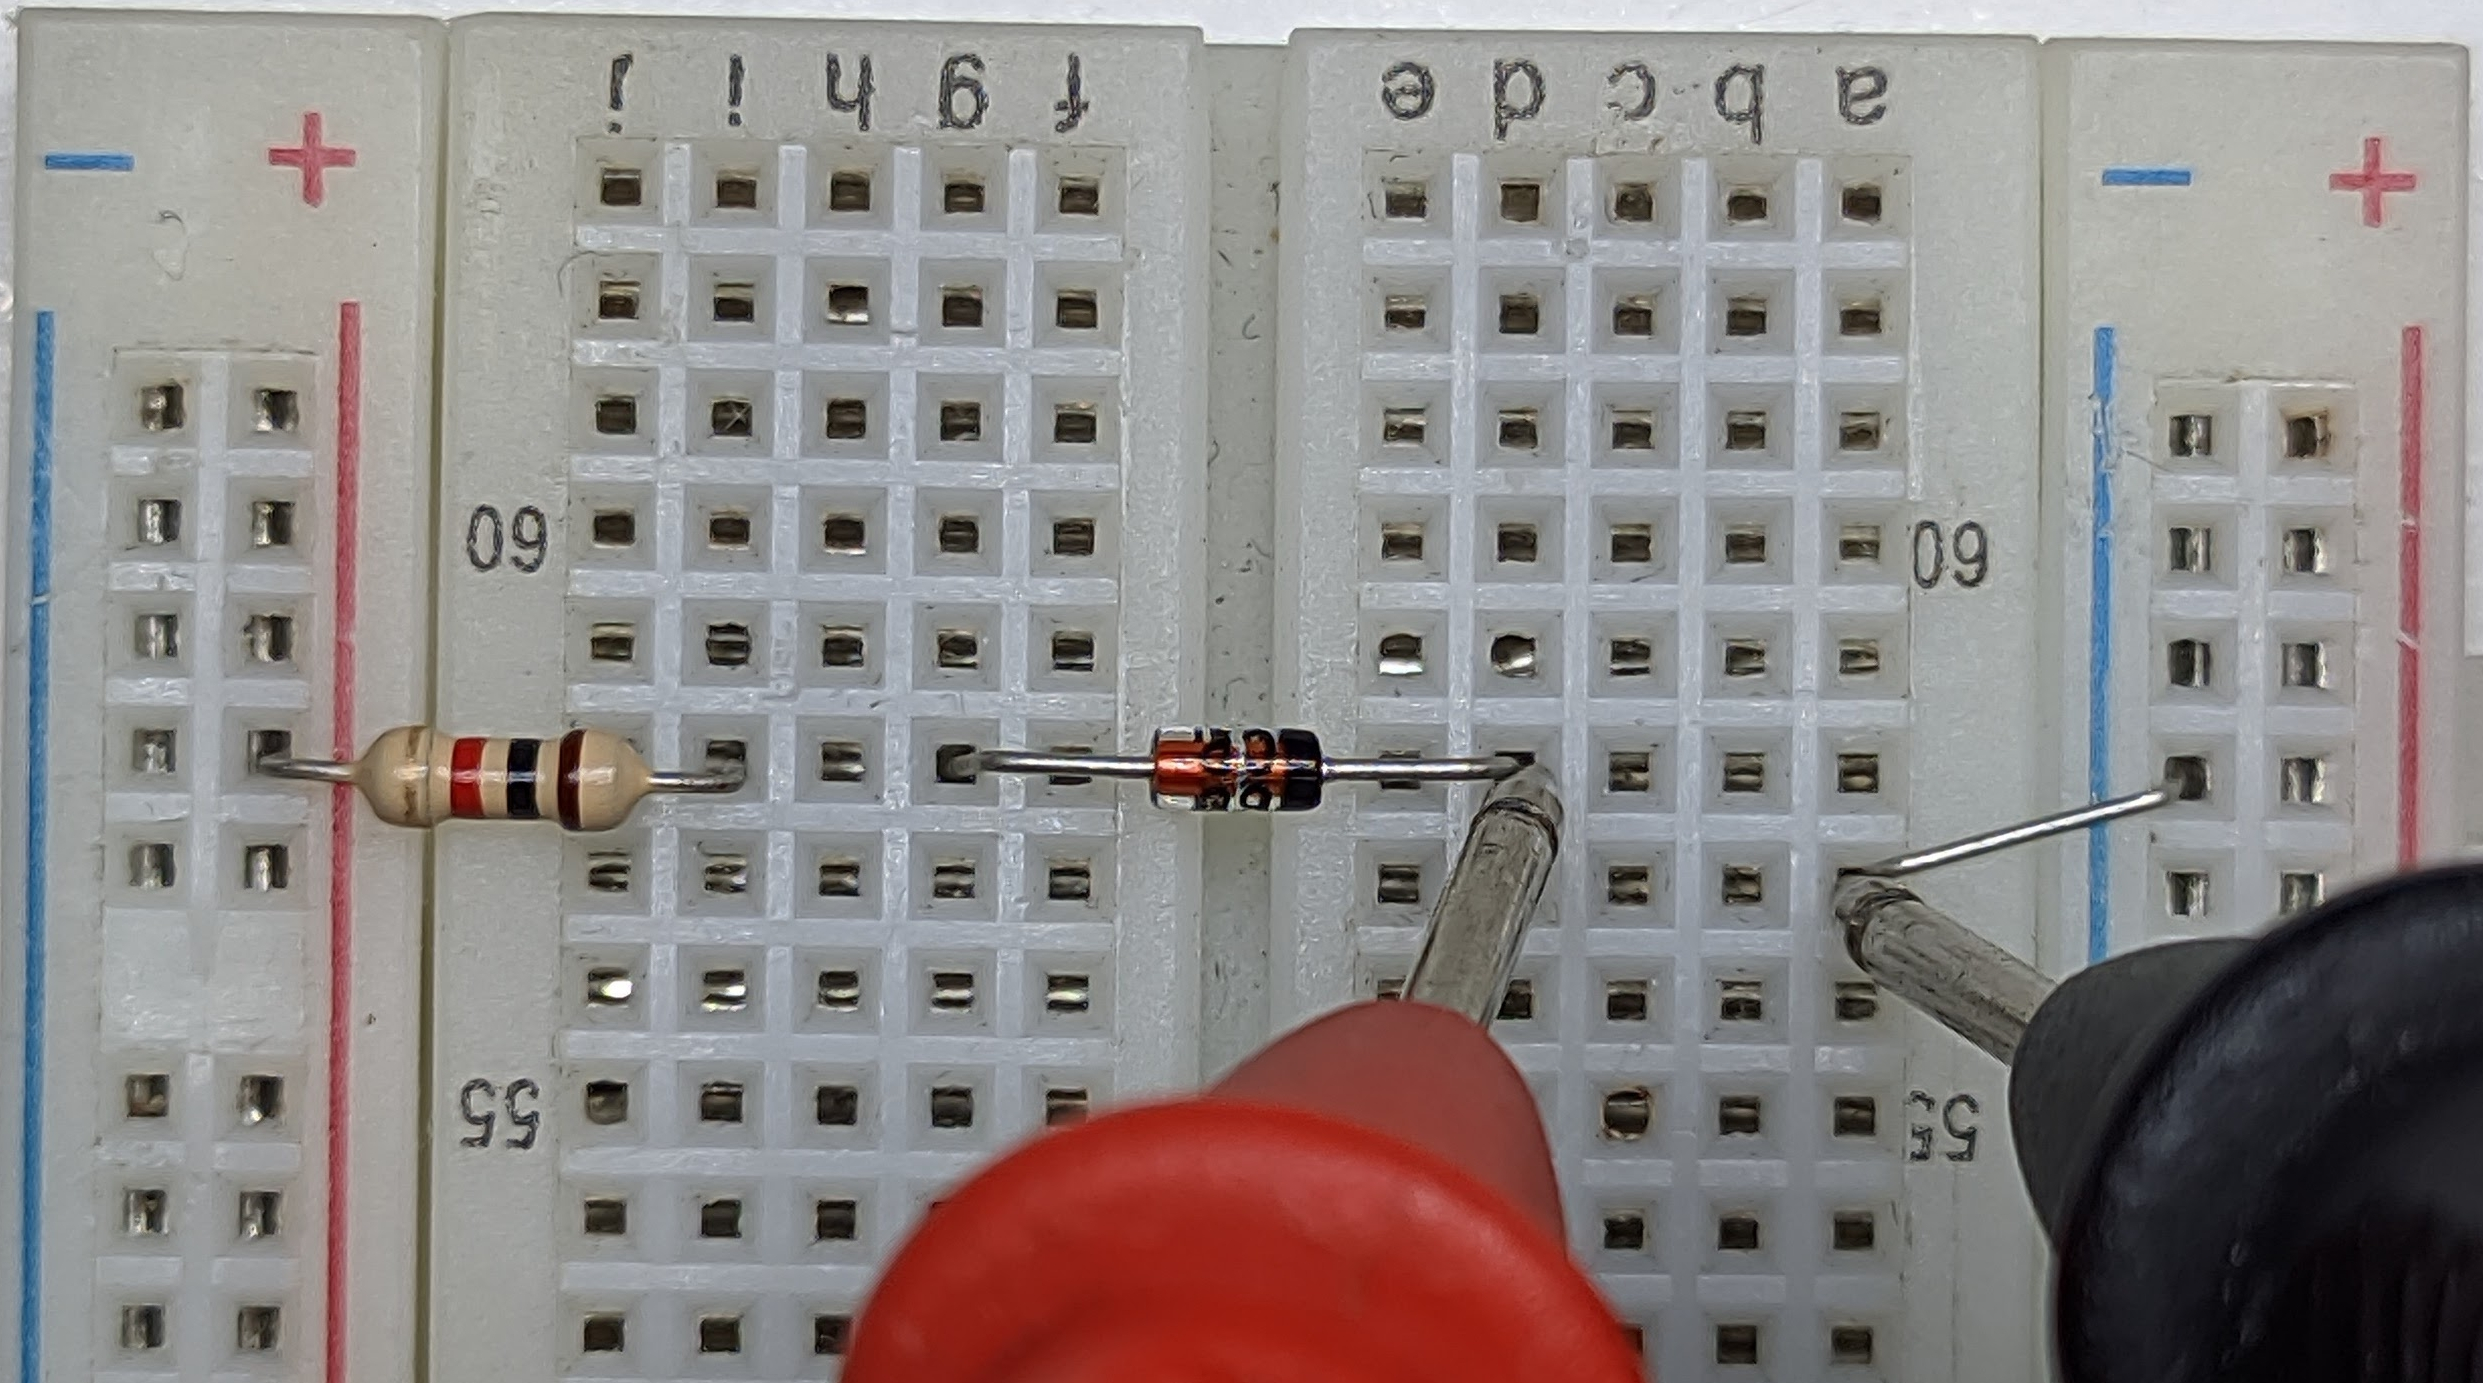
\includegraphics[angle=180, width=1\textwidth]{pictures/prot_crkt-2_curr.jpg}
          \caption{Medicion de corriente del circuito.}
          \label{crkt.Ge.mult.curr}
        \end{minipage}
        \begin{minipage}{0.3\textwidth}
          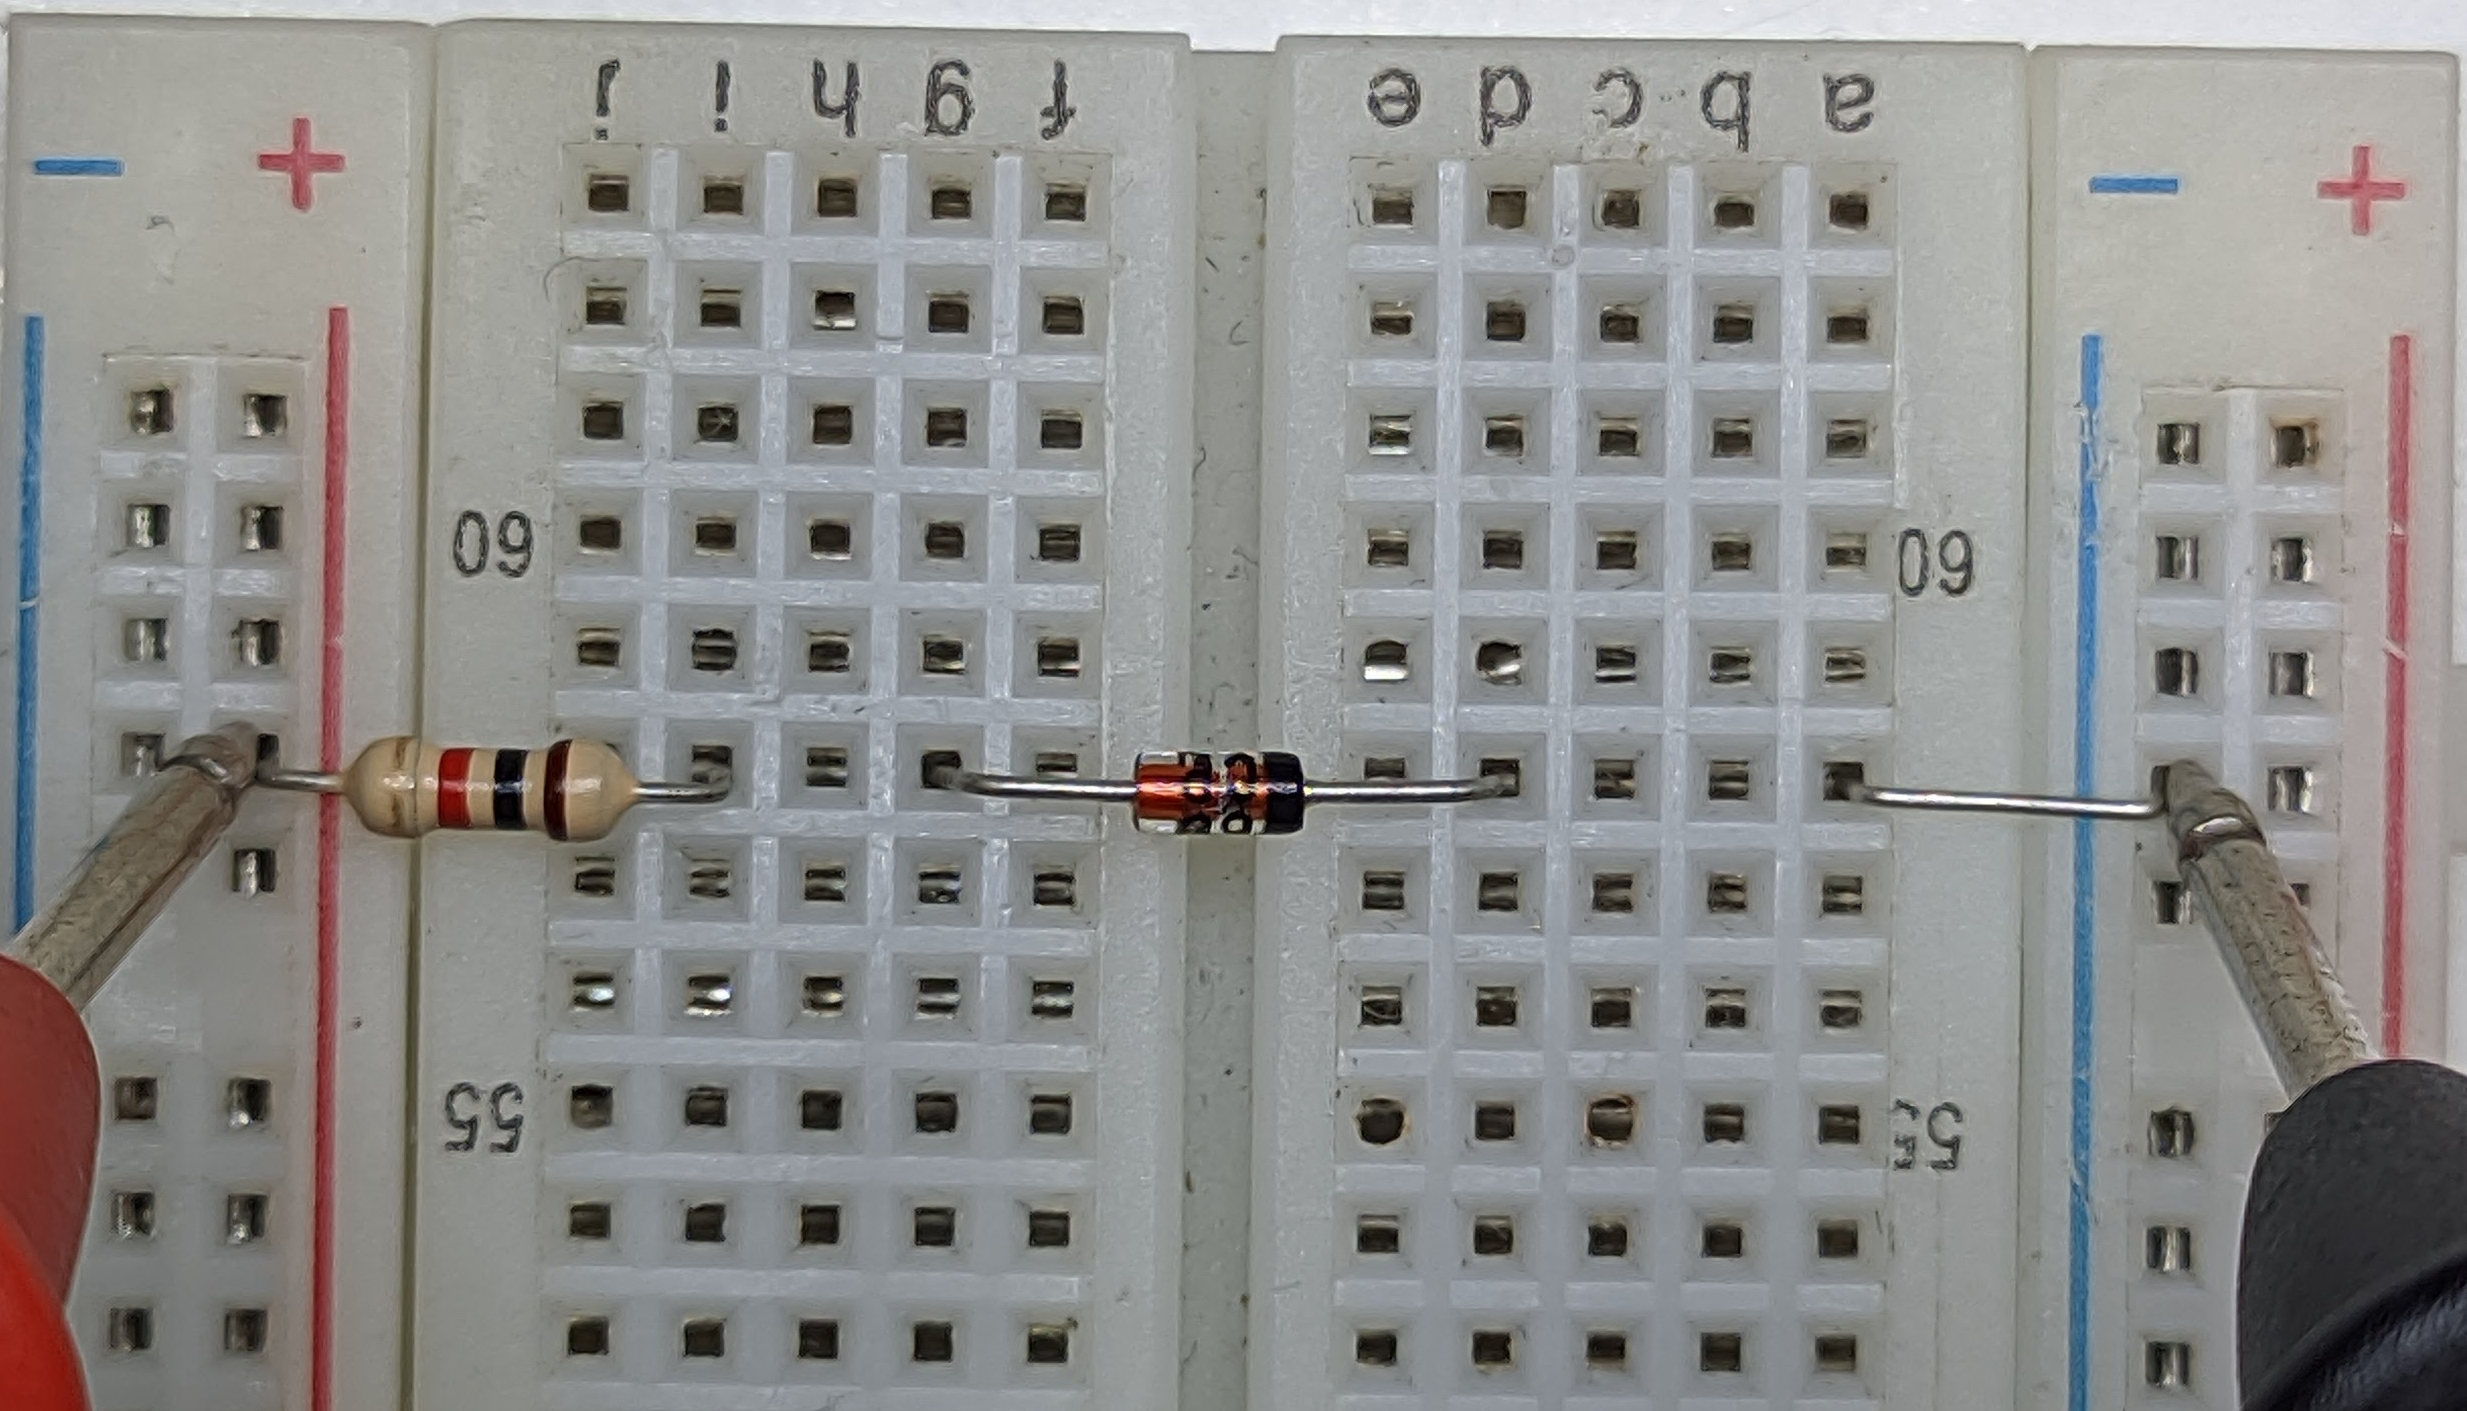
\includegraphics[angle=180, width=1\textwidth]{pictures/prot_crkt-2_vi.jpg}
          \caption{Medicion de tension de la fuente.}
          \label{crkt.Ge.mult.vi}
        \end{minipage}
        \begin{minipage}{0.3\textwidth}
          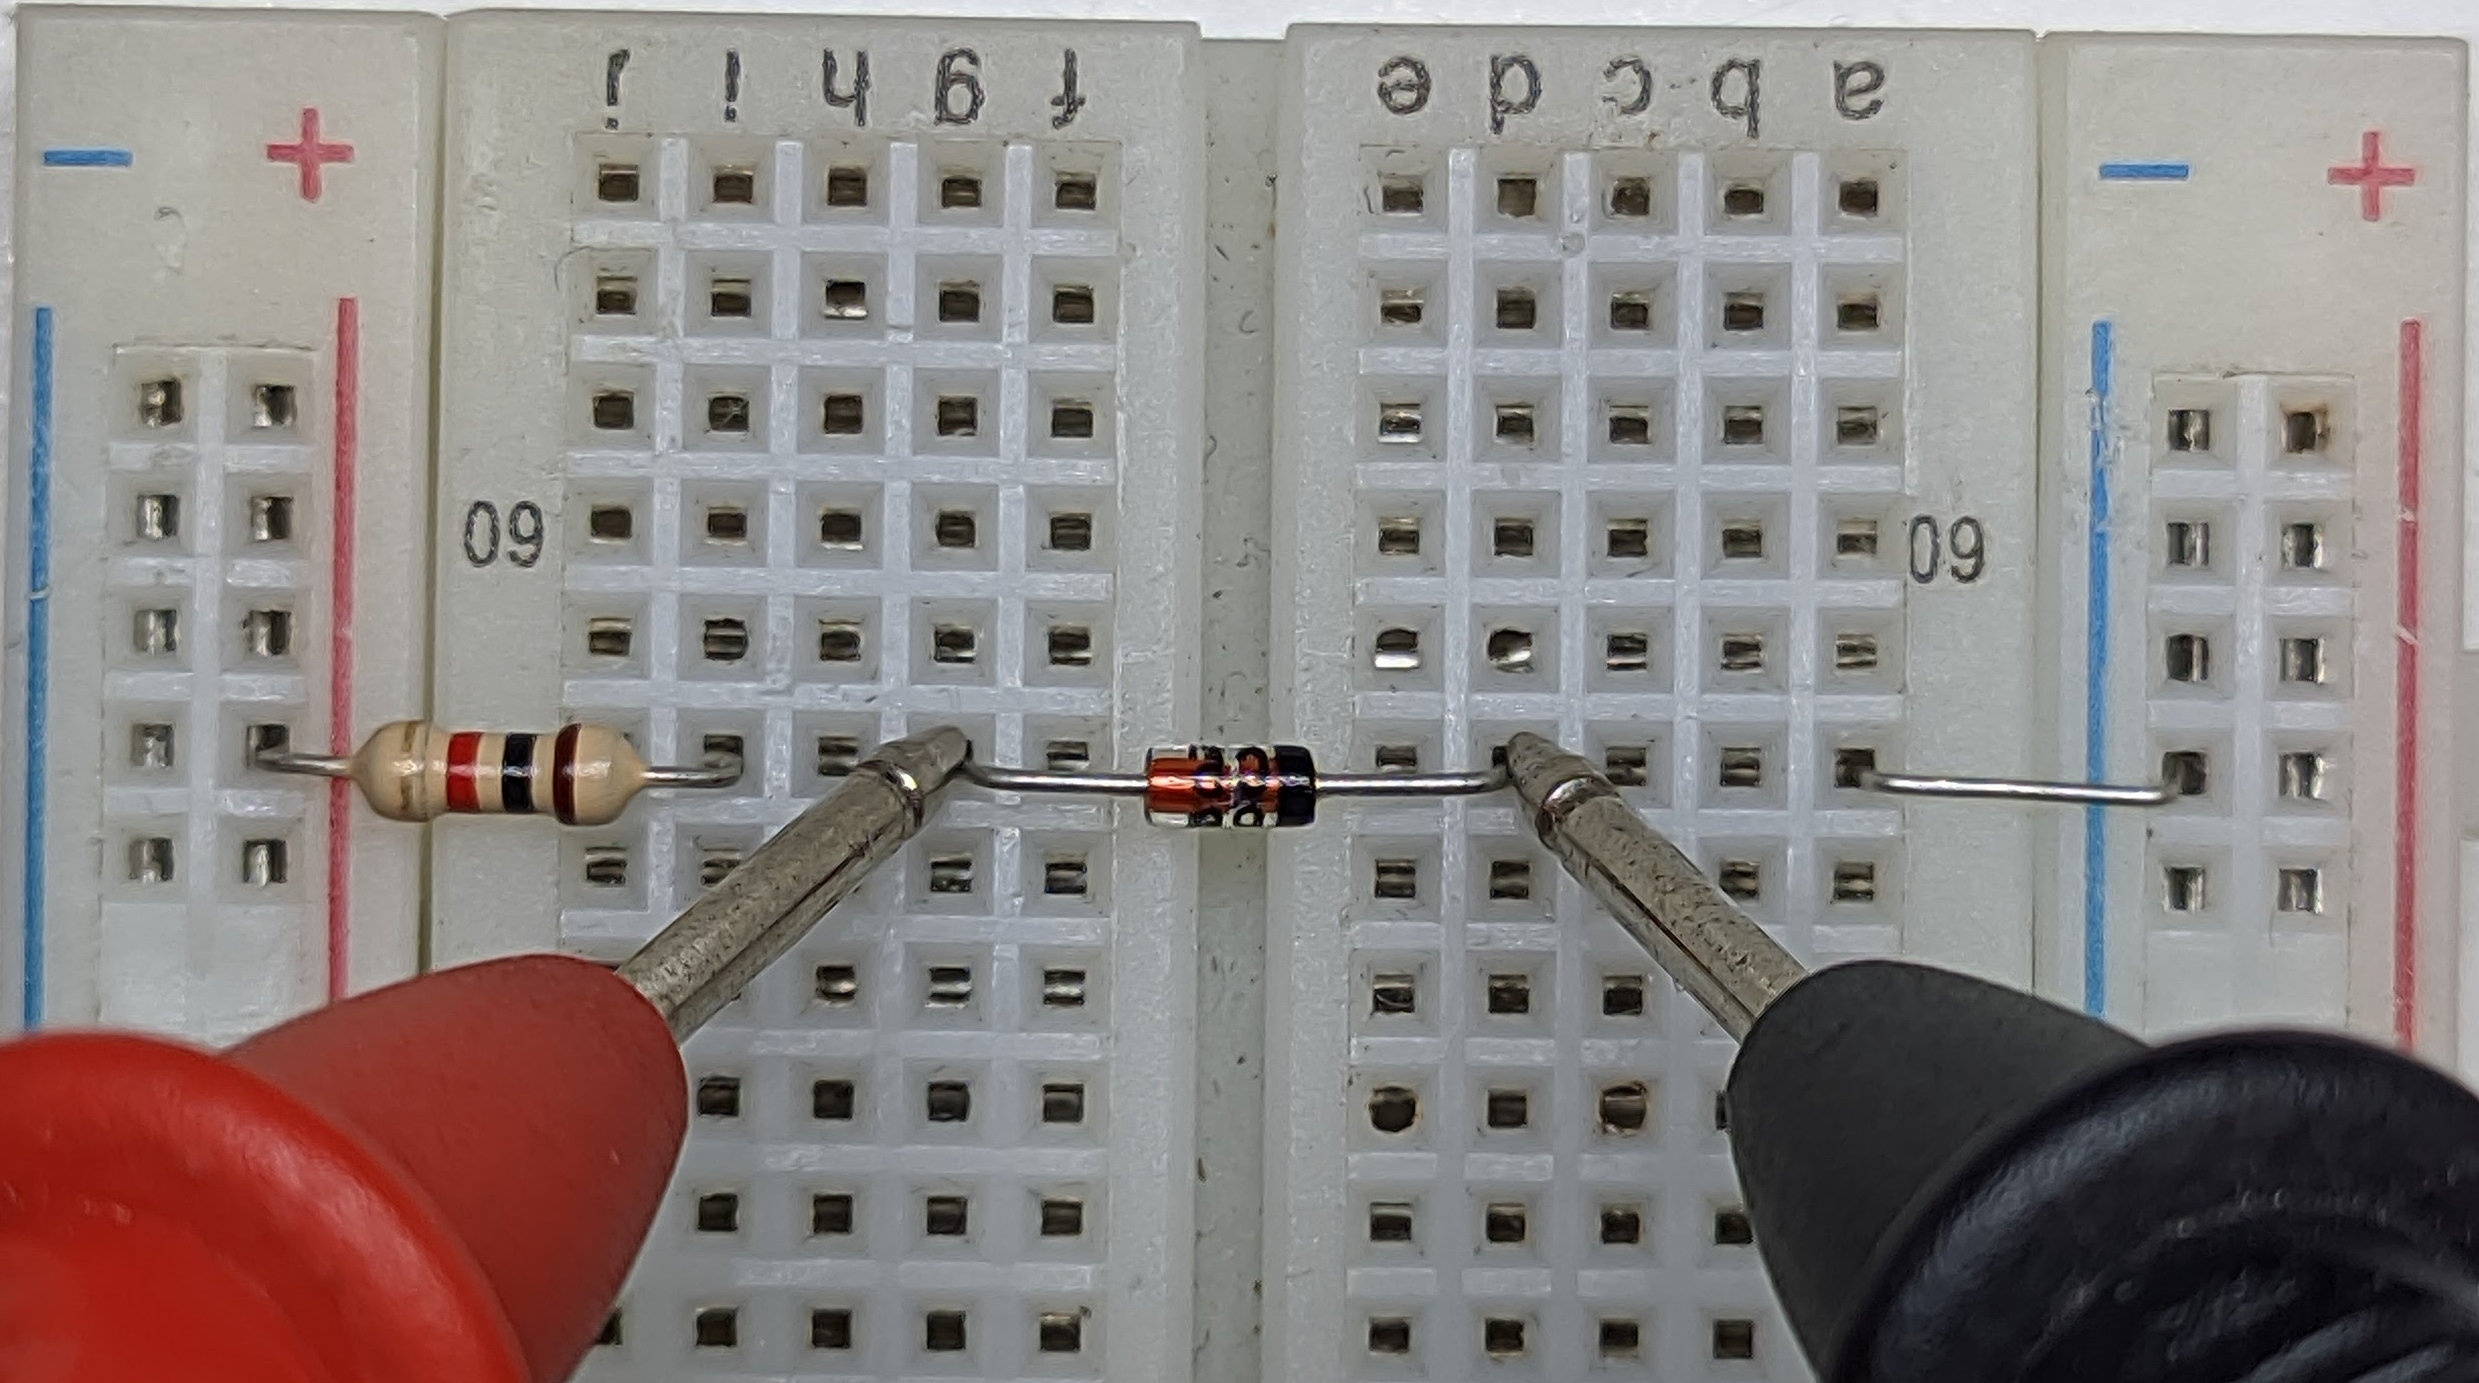
\includegraphics[angle=180, width=1\textwidth]{pictures/prot_crkt-2_vd.jpg}
          \caption{Medicion de caida de tension del diodo.}
          \label{crkt.Ge.mult.vd}
        \end{minipage}
      \end{figure}

      Con el circuito de la figura (\ref{crkt.Ge.prot}), y los tres multimetros midiendo al mismo tiempo, procedimos a
      hacer las variaciones de voltaje de entrada y tomar muestras de todas los valores.

      \begin{figure}[!ht]
        \centering
        \begin{minipage}{0.25\textwidth}
          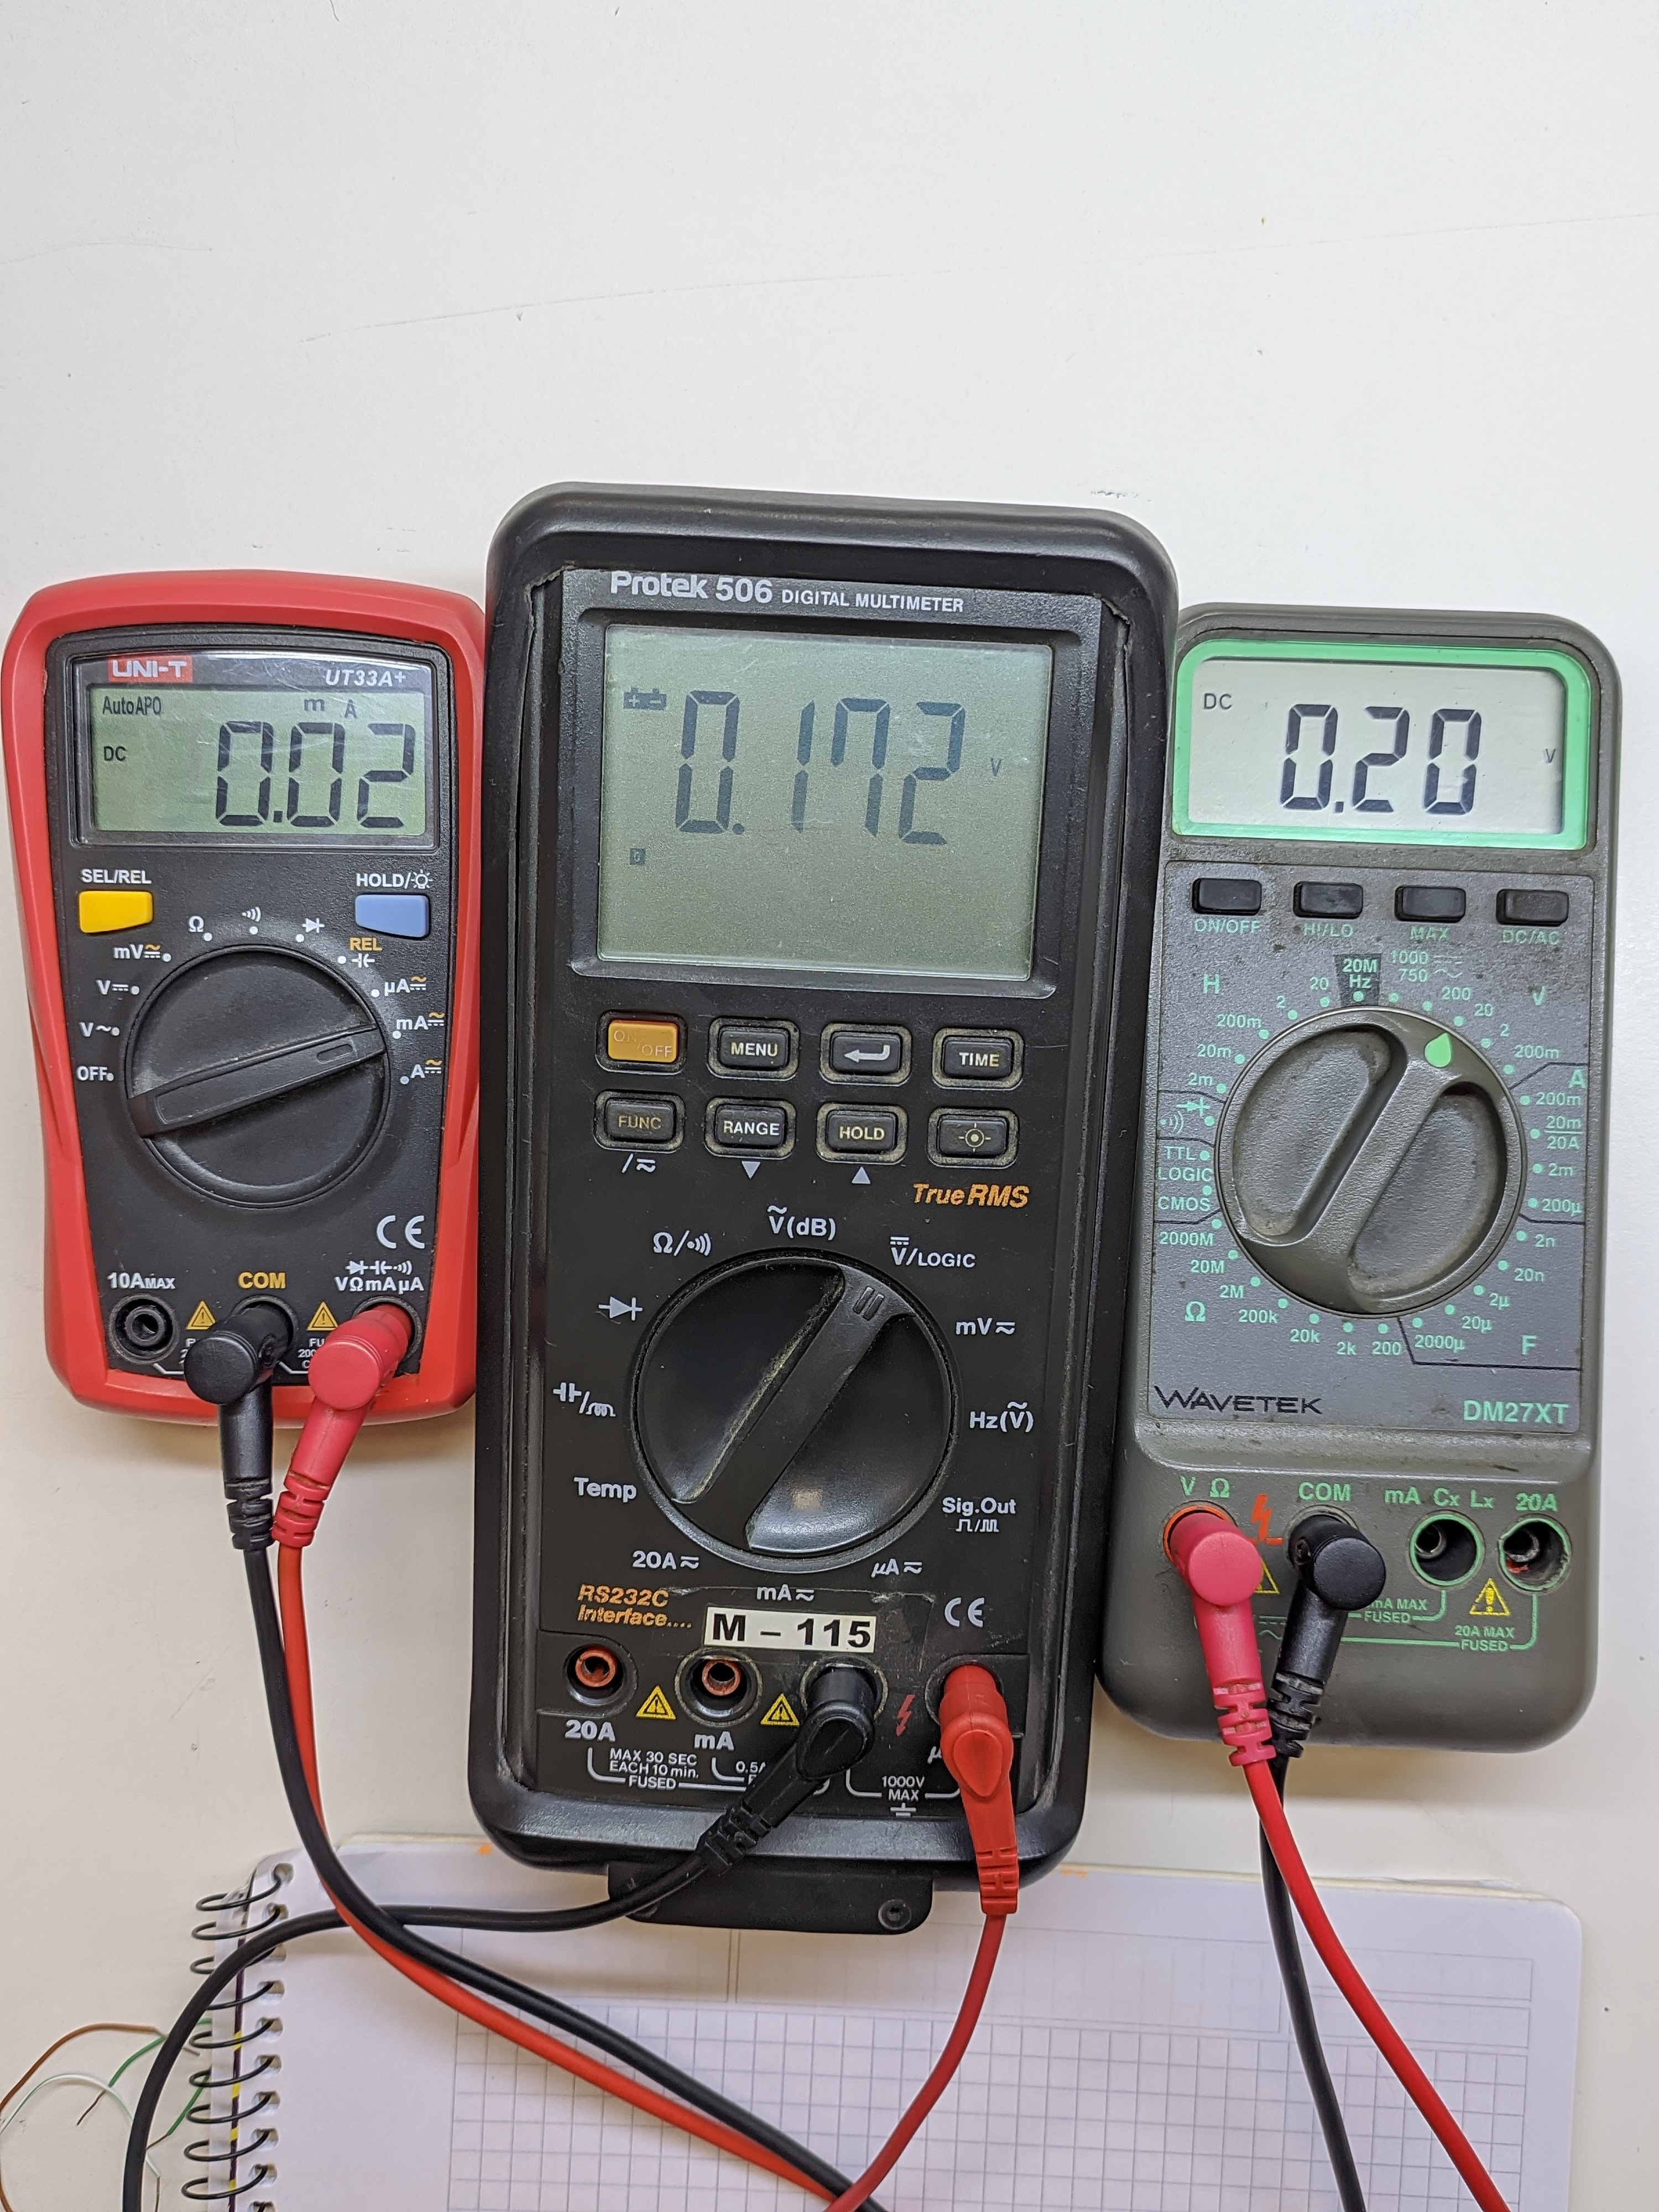
\includegraphics[width=1\textwidth]{pictures/mult_crkt-2_03.jpg}
        \end{minipage}
        \begin{minipage}{0.25\textwidth}
          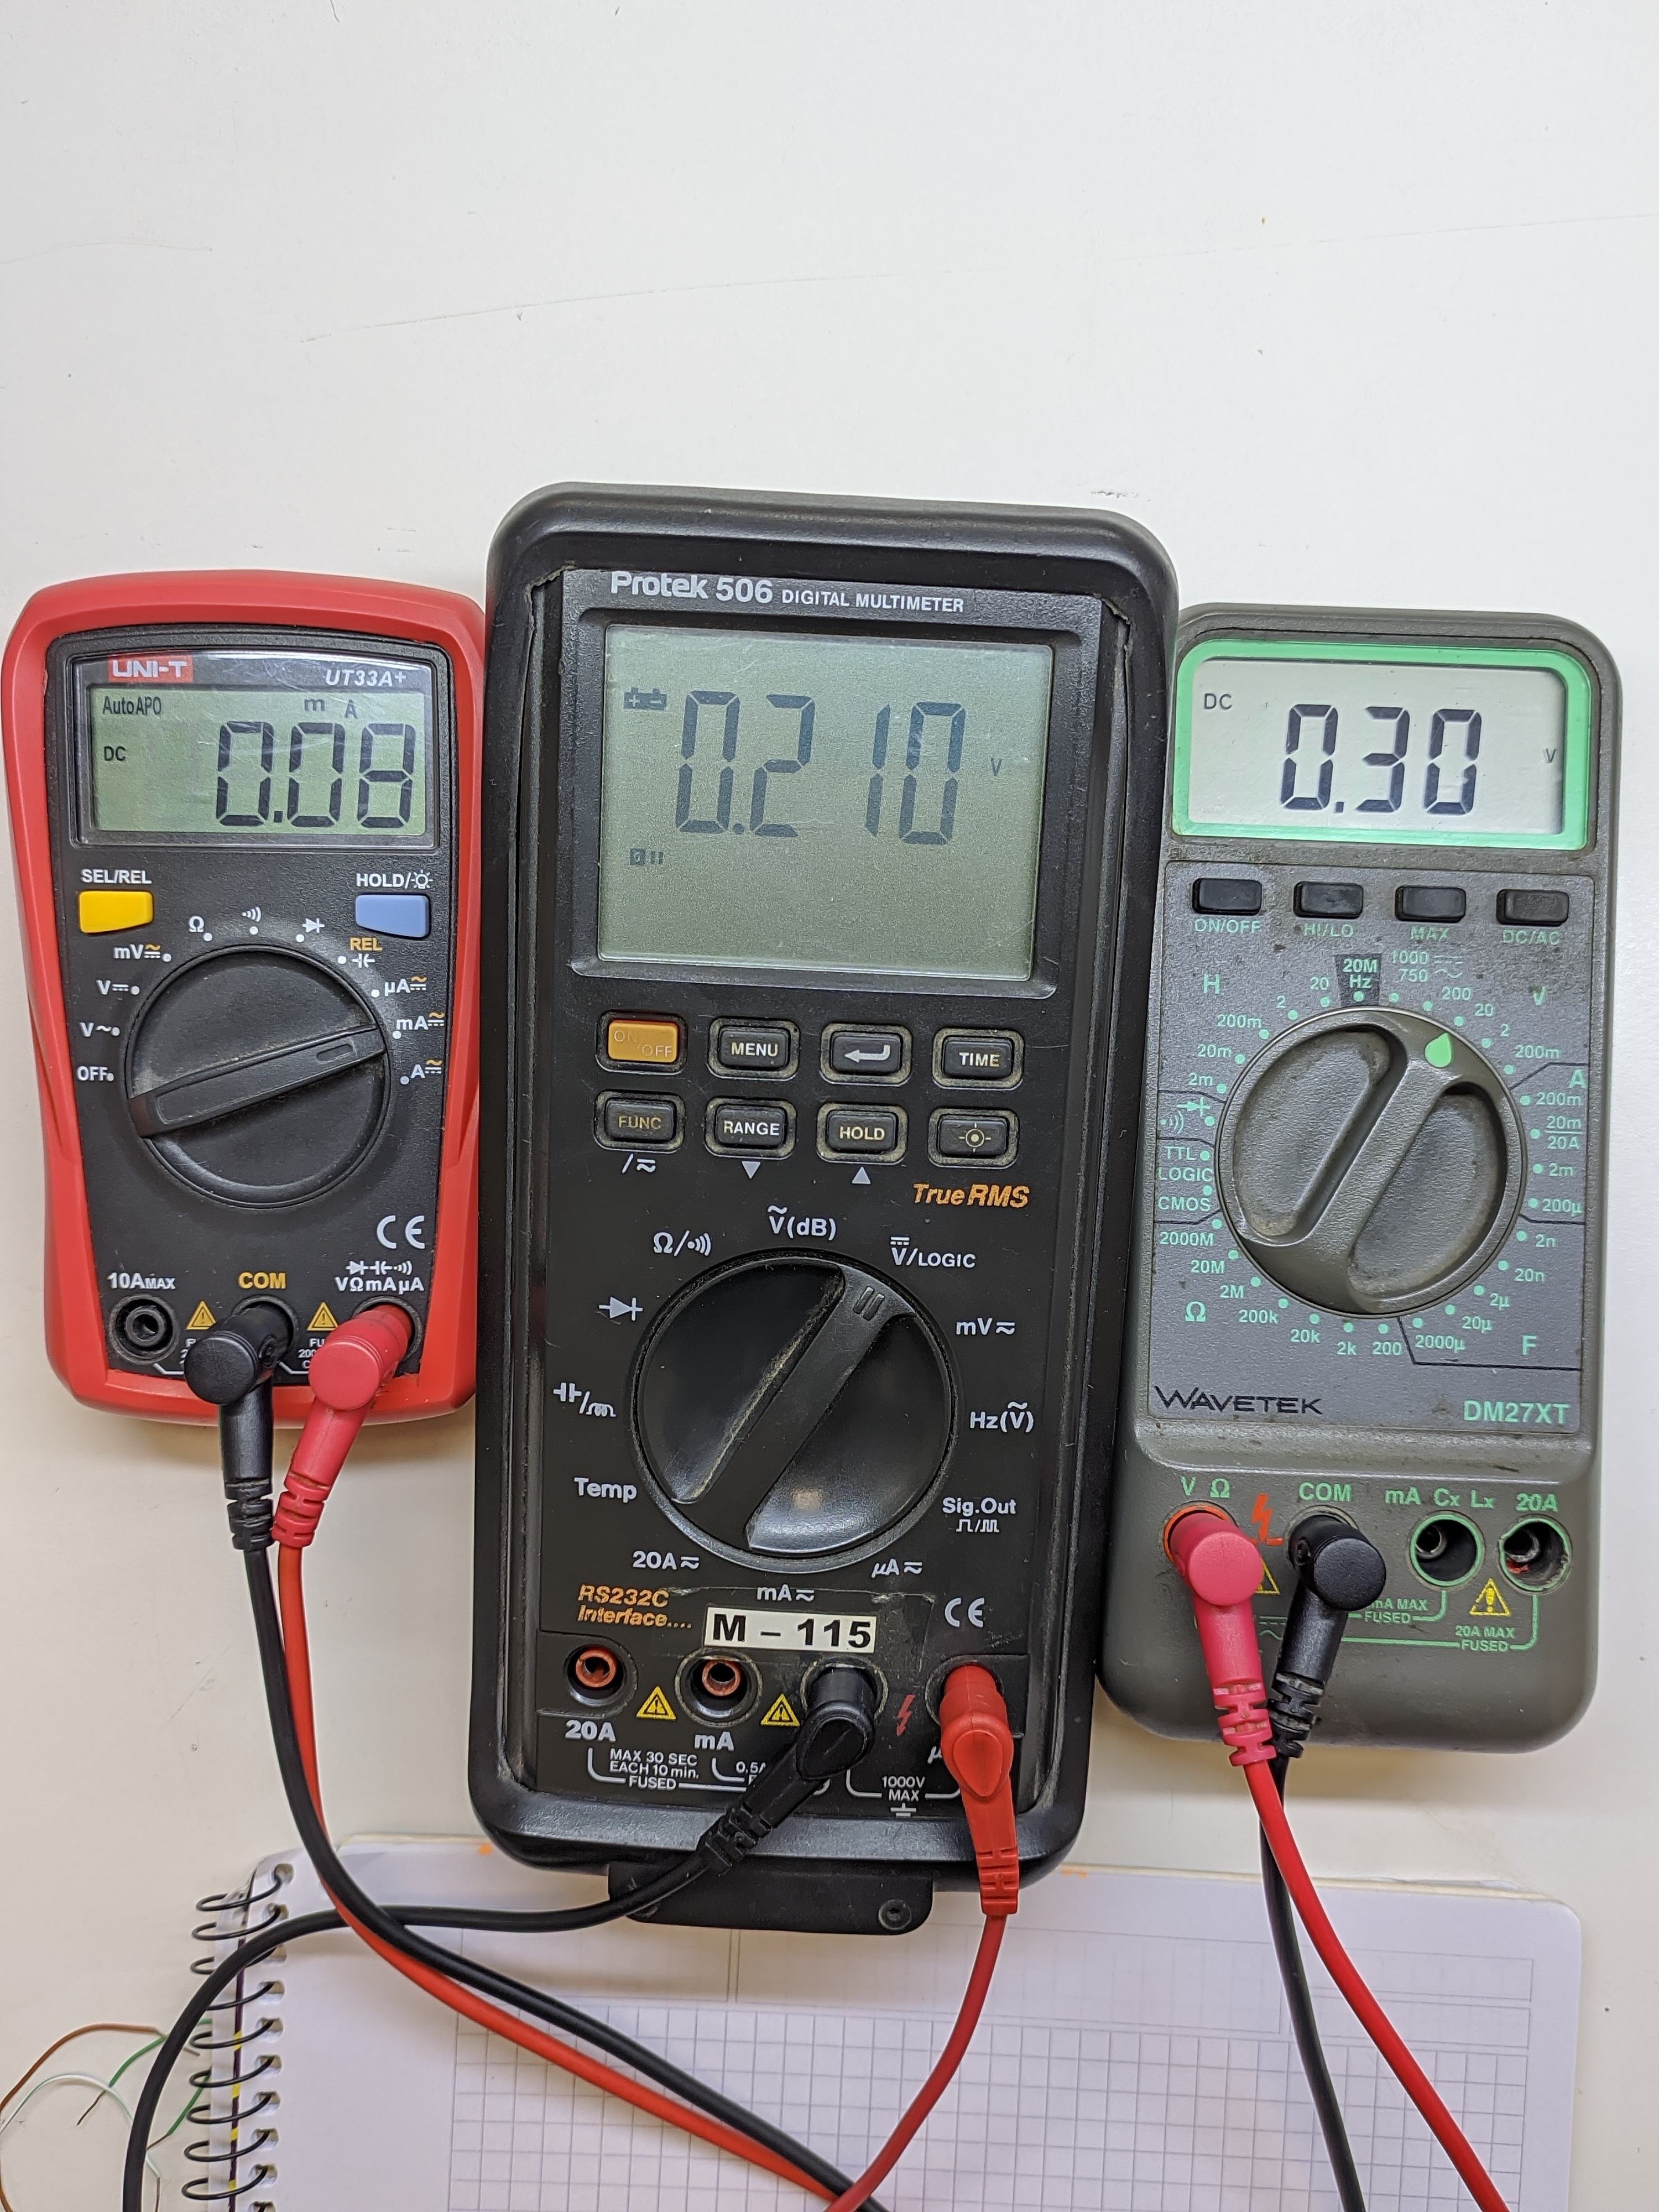
\includegraphics[width=1\textwidth]{pictures/mult_crkt-2_05.jpg}
        \end{minipage}
        \begin{minipage}{0.25\textwidth}
          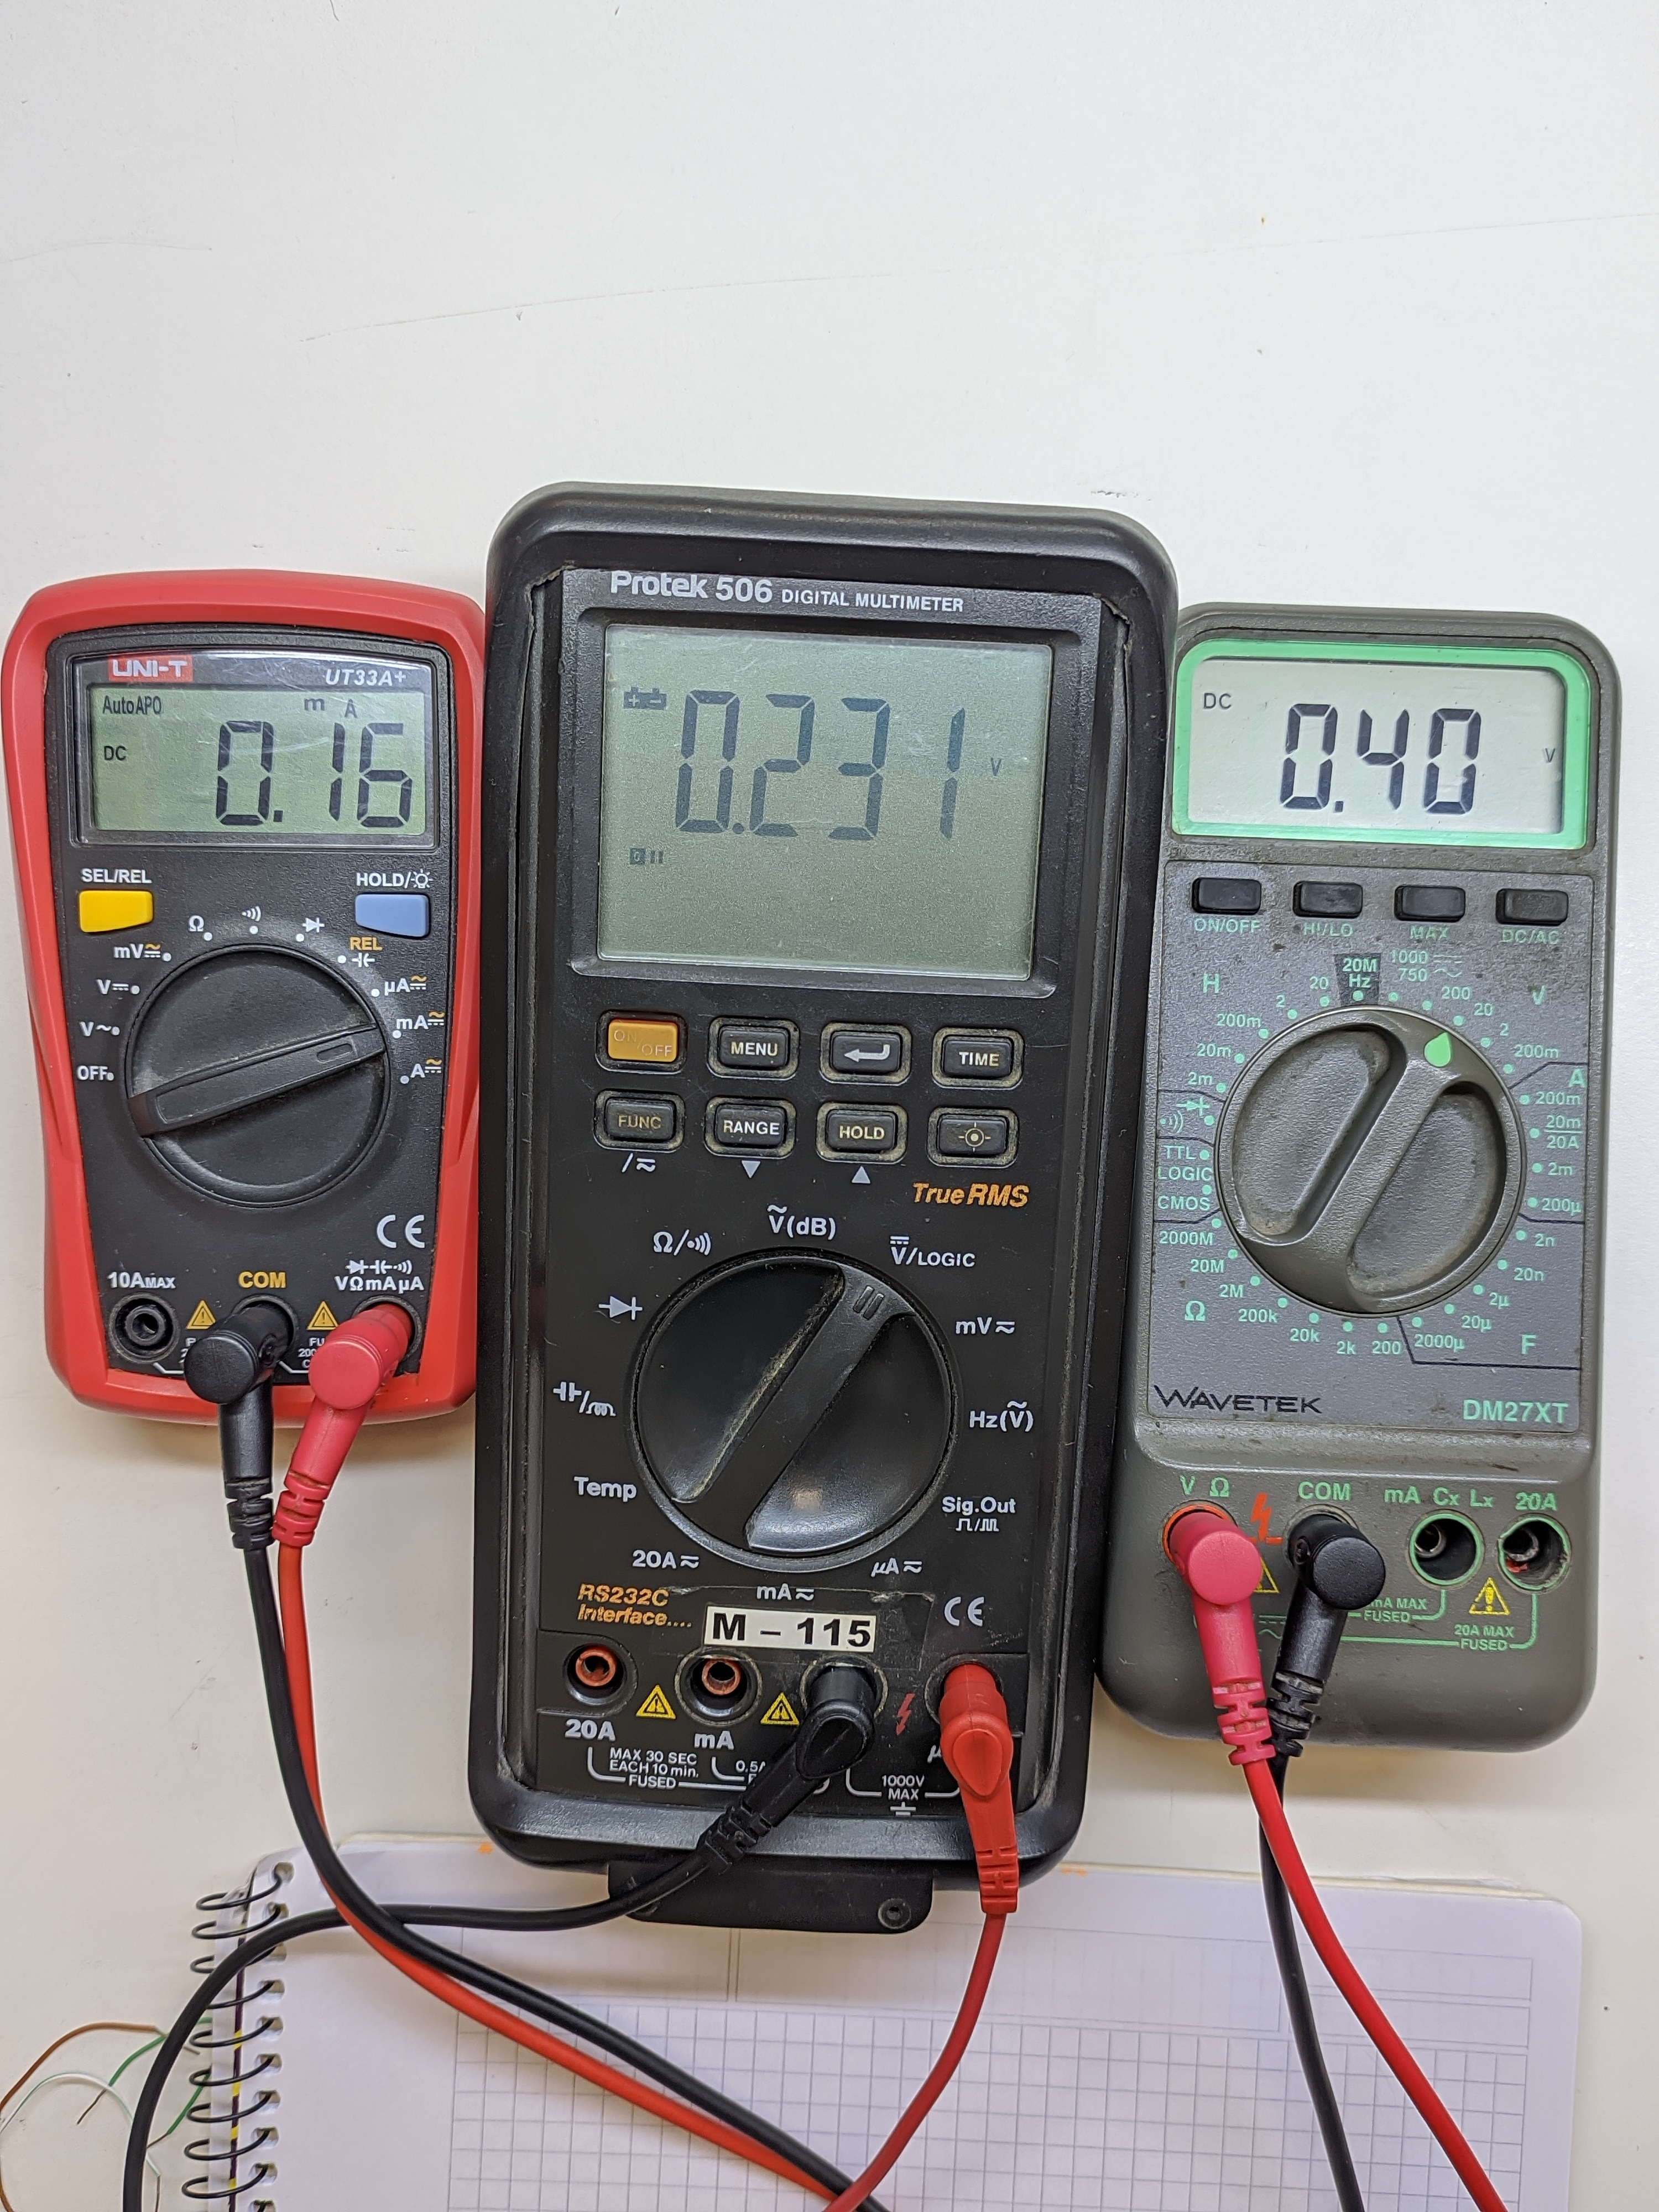
\includegraphics[width=1\textwidth]{pictures/mult_crkt-2_07.jpg}
        \end{minipage}
        \caption{Algunas fotos de las mediciones de los tres multimetros. El de la izquierda mide corriente en mA, el
        del medio mide la caida de tension del diodo y el de la derecha mide la entrada de la fuente}
      \end{figure}

      \begin{table}[H]
        \resizebox{\textwidth}{!}{\begin{tabular}{|c|c|c|c|c|c|c|c|c|c|c|c|c|c|c|}
          \hline
          $V_{in}$ & 110mV  & 160mV & 200mV   & 250mV & 300mV   & 350mV & 400mV   & 450mV & 500mV & 600mV      & 800mV      & 1V & 3V & 5V\\
          \hline
          $I_t$    & 0A     & 0A    & 0.02mA & 0.05mA & 0.08mA  & 0.12mA & 0.16mA & 0.21mA & 0.26mA & 0.35mA  & 0.54mA  & 0.73mA & 2.73mA & 4.69mA\\
          \hline
          $v_D$    & 100mV  & 150mV & 170mV   & 190mV & 210mV   & 220mV & 230mV   & 240mV & 240mV & 250mV   & 270mV   & 280mV & 330mV & 370mV\\
          \hline
        \end{tabular}}
        \caption{Tabla de valores medidos del diodo de germanio.}
        \label{table.Ge}
      \end{table}

      Con los datos de la tabla (\ref{table.Ge}), podemos hacer una curva y compararla con la curva simulada.
      \begin{figure}[!ht]
        \centering
        \begin{tikzpicture}
          \begin{axis}[
            width=14cm,
            height=7cm,
            xlabel={$v_D$ [V]},
            ylabel={$i_D$ [mA]},
            grid=both,
            minor tick num=1,
            scale only axis,
            enlargelimits=false,
            scaled ticks=false,
            restrict x to domain=-0.2:1,
          ]
          \addplot[
            color=blue,
            mark=none,
            thick,
          ] table[
            col sep=tab,
            header=true,
            x=V(d1),
            y expr=\thisrow{I(D1)}*1000
          ] {simulations/TP2_2_graph.txt};
          \addlegendentry{Simulada}
          \addplot[
            color=red,
            mark=none,
            thick,
          ] coordinates {(0.1, 0)(0.15, 0)(0.17, 0.02)(0.19, 0.05)(0.21, 0.08)(0.22, 0.12)(0.23, 0.16)(0.24, 0.21)(0.245, 0.26)(0.25, 0.35)(0.27, 0.54)(0.28, 0.73)(0.33, 2.73)(0.37, 4.96)};
          \addlegendentry{Medida}
          \end{axis}
        \end{tikzpicture}
        \caption{Grafico de la curva caracteristica simulada y la medida experimentalmente del diodo de Germanio.}
        \label{graph.comparativa.Ge}
      \end{figure}

      Como se puede ver, la figura (\ref{graph.comparativa.Ge}), no parece tener tantas similitudes con la curva
      simulada. Esto puede ser porque el diodo 1N60 fue descontinuado hace muchos años, y fue reemplazado por otro
      diodo. Es muy posible que este nuevo diodo tenga otras caracteristicas diferentes, como por ejemplo menor
      resistencia interna cuando se pone en conduccion. Tambien puede ser un problema del modelo. No hay un modelo
      oficial provisto por un fabricante de semiconductores.

      \section{Comparativa de las dos curvas medidas}
      \begin{figure}[!ht]
        \centering
        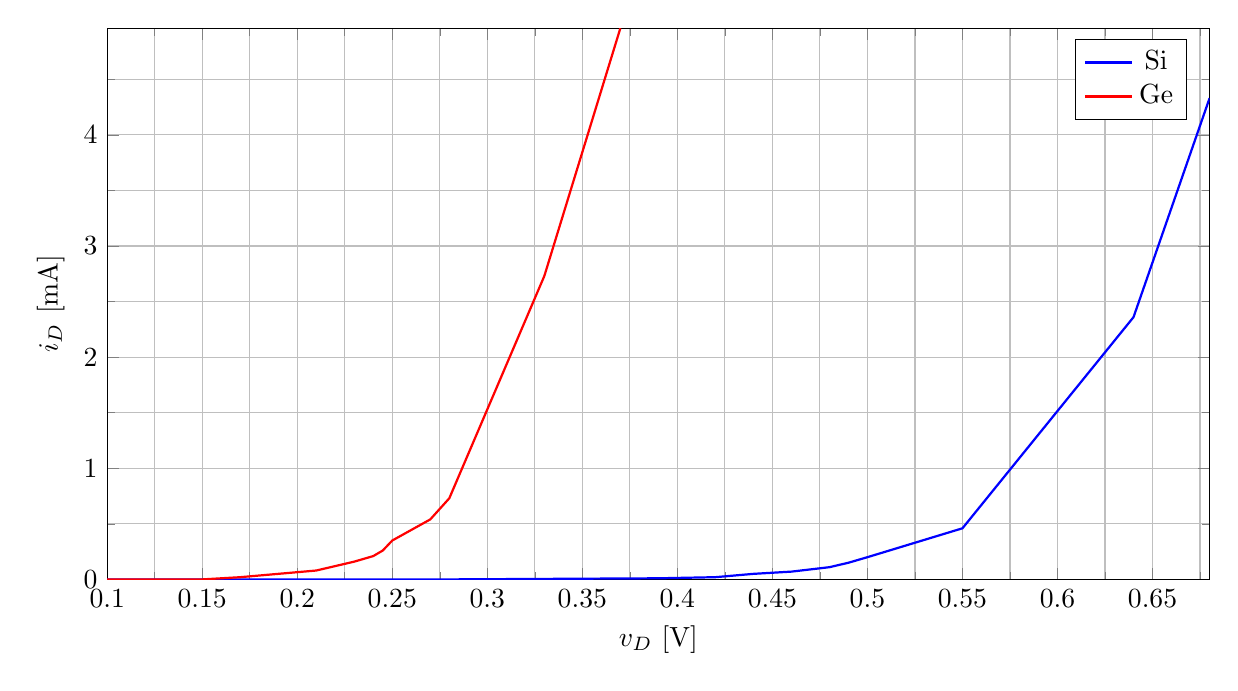
\begin{tikzpicture}
          \begin{axis}[
            width=14cm,
            height=7cm,
            xlabel={$v_D$ [V]},
            ylabel={$i_D$ [mA]},
            grid=both,
            minor tick num=1,
            scale only axis,
            enlargelimits=false,
            scaled ticks=false,
            restrict x to domain=-0.2:1,
          ]
          \addplot[
            color=blue,
            mark=none,
            thick,
          ] coordinates {(.1, 0)(.28, 0)(.39, 0.01)(.42, 0.02)(.44, 0.05)(.46, 0.07)(.48, 0.11)(.49, 0.15)(.5, 0.2)(0.55, 0.46)(0.64, 2.36)(0.68, 4.33)};
          \addlegendentry{Si}
          \addplot[
            color=red,
            mark=none,
            thick,
          ] coordinates {(0.1, 0)(0.15, 0)(0.17, 0.02)(0.19, 0.05)(0.21, 0.08)(0.22, 0.12)(0.23, 0.16)(0.24, 0.21)(0.245, 0.26)(0.25, 0.35)(0.27, 0.54)(0.28, 0.73)(0.33, 2.73)(0.37, 4.96)};
          \addlegendentry{Ge}
          \end{axis}
        \end{tikzpicture}
        \caption{Grafico de la curva caracteristica medida del diodo de Germanio y Silicio.}
        \label{graph.comparativa.medida}
      \end{figure}

      En la figura (\ref{graph.comparativa.medida}), nuevamente podemos apreciar las diferencias en los codos de
      conmutacion de ambos semiconductores. Las ventajas y desventajas son las mismas que cuando se hizo la comparativa
      de la figura (\ref{graph.simulation.comparativa.directa}).

  \part{Comportamiento del diodo en función de la temperatura}
    \chapter{Actividad de simulacion}
        Se pide simular el diodo 1N3198 pero esta vez para poder corroborar como afecta la temperatura la curva
        caracteristica. Para la simulacion se utilizaran las siguientes temperaturas: $20°C$, $100°C$ y $125°C$. Ademas
        de los siguientes parametros que se muestran a continuacion con el circuito a simular

        \begin{figure}[!ht]
          \centering
          \begin{minipage}{0.45\textwidth}
            \begin{circuitikz}[american voltages]
              \draw (0, -1) to [V=$V_1$, invert]             (0, 3)
                            to [short, -, i>^=$i_D$]         (1, 3)
                            to [R=$R_1$, v=$V_{R_1}$]        (4, 3)
                            to [short, -]                    (5, 3)
                            to [zzD=$1N3198$, v=$v_D$]       (5, -1)
                            to [short, -]                    (5, -1)
                            to [short, -]                    (0, -1)
                            ;
            \end{circuitikz}
            \caption{Circuito con diodo de silicio 1N3198.}
            \label{crkt.zener.directa}
          \end{minipage}
          \hfill
          \begin{minipage}{0.45\textwidth}
            \begin{lstlisting}[style=ltspice, caption={Parámetros de simulación LTspice}, label=list.zenner.directa]
              .dc V1 0 800m 10m
              .model 1N3198 D (IS=2.0e-7 N=1.20 RS=1.0 EG=1.11 XTI=-2 CJO=40p VJ=0.75 M=0.333 BV=2.25 IBV=5m KF=0 AF=1 FC=0.5)
              .step temp list 20 100 125
            \end{lstlisting}
          \end{minipage}
        \end{figure}


        A continuacion se presenta el grafico con cada variante de la curva caracteristica con su respectiva temperatura:






        Se puede observar y comprobar lo visto en el marco teorico, a mayor temperatura que se le aplique al diodo,
        el codo de conmutacion se puede observar con menor voltaje aplicado sobre el circuito, asi como lo afecta
        cuando aumenta la temperatura tambien lo afecta a menor temperatura, siendo asi que el diodo necesita mas
        voltaje para lograr pasar al estado de conmutacion. Sabiendo que los graficos que nos brinda el
        fabricante en la hoja de datos es en una temperatura promedio de 25$°C°$ en el grafico se observa
        perfectamente  los otros 2 casos.



        A su vez hay otra variable que termina siendo afectada por la temperatura y esta es la corriente de fuga,
        sabiendo que esto es la pequeña corriente que fluye cuando el diodo está polarizado en inversa. Idealmente
        debería ser cero, pero debido a la generación de pares electrón-hueco en el material, existe una pequeña
        corriente. La corriente de fuga inversa aumenta exponencialmente con la temperatura, aproximadamente se
        duplica por cada aumento de 10$°C$, esto se debe a que el aumento de la temperatura reduce la zona de
        agotamiento del semiconductor PN, provocando tambien que la barrera de potencial disminuya (por eso a mayor
        temperatura se logra conmutar con menor voltaje), facilitando el paso de los electrones a traves de esta
        generando la corriente de fuga.





  \part{Circuitos recortadores con diodos Zener}
    \chapter{Actividad de simulacion}
        En este ejercicio se pide analizar dos circuitos compuestos por dos diodos zener configurados como
        "back-to-back" implica conectar dos diodos Zener en sentido opuesto, con el ánodo de un diodo conectado al
        cátodo del otro. Esta configuracion se utiliza principalmente para proteger contra sobretensiones en ambas
        polaridades.

        \subsection{Circuito 1}

            En el primer circuito  se plantea lo siguiente:

            \begin{figure}[!ht]
              \centering
              \begin{minipage}{0.45\textwidth}
                \begin{circuitikz}[american voltages]
                  \draw (0, -1) to [V=$V_1$]                     (0, 3)
                                to [short, -, i<^=$i_D$]         (1, 3)
                                to [R=$R_1$, v<=$V_{R_1}$]       (4, 3)
                                to [short, -]                    (5, 3)
                                to [zzD=$1N60$, v<=$v_D$]        (5, -1)
                                to [short, -]                    (5, -1)
                                to [short, -]                    (0, -1)
                                ;
                \end{circuitikz}
                \caption{Circuito con diodo de silicio 1N60 en inversa.}
                \label{crkt.recortador.btb}
              \end{minipage}
              \hfill
              \begin{minipage}{0.45\textwidth}
                \begin{lstlisting}[style=ltspice, caption={Parámetros de simulación LTspice}, label=list.recortador.btb]
                  .model 1N5338B D(IS=1n RS=1 N=1.3 BV=5.1 IBV=240m CJO=200p TT=1u)
                  .model 1N5357B D(IS=1n RS=1 N=1.3 BV=20 IBV=65m CJO=200p TT=1u)
                  .tran .04
                \end{lstlisting}
              \end{minipage}
            \end{figure}



            Y el grafico que presenta es el siguiente:



            Como se puede observar, los diodos zener recortan las ondas dependiendo de los valores de los mismos, en
            este caso los diodos son de 5.1$V$ y 20$V$. En el semiciclo positivo, el Zener de 20$V$ está en inversa y
            conduce solamente si $Vin > 20.7V$, por otro lado en el semiciclo negativo, el Zener de 5.1$V$ esta en
            inversa y conduce solamente si $Vin <-5.8V$. Por lo tanto recorta la señal entre $+20.7V$ y $-5.8V$.


        \subsection{Circuito 2}

            En el segundo circuito se plantea lo siguiente:

            \begin{figure}[!ht]
              \centering
              \begin{minipage}{0.45\textwidth}
                \begin{circuitikz}[american voltages]
                  \draw (0, -1) to [V=$V_1$]                     (0, 3)
                                to [short, -, i<^=$i_D$]         (1, 3)
                                to [R=$R_1$, v<=$V_{R_1}$]       (4, 3)
                                to [short, -]                    (5, 3)
                                to [zD=$1N60$, v<=$v_D$]          (5, -1)
                                to [short, -]                    (5, -1)
                                to [short, -]                    (0, -1)
                                ;
                \end{circuitikz}
                \caption{Circuito con diodo de silicio 1N60 en inversa.}
                \label{crkt.recortador.ftf}
              \end{minipage}
              \hfill
              \begin{minipage}{0.45\textwidth}
                \begin{lstlisting}[style=ltspice, caption={Parámetros de simulación LTspice}, label=list.recortador.ftf]
                  .model 1N5342B D(IS=1n RS=1 N=1.3 BV=6.8 IBV=175m CJO=200p TT=1u)
                  .model 1N5349B D(IS=1n RS=1 N=1.3 BV=12 IBV=100m CJO=200p TT=1u)
                  .tran .04
                \end{lstlisting}
              \end{minipage}
            \end{figure}



            Y el grafico que presenta es el siguiente:

            En este caso al variar los valores de los diodos zener lo que ocurre es lo siguiente: Se presentan dos
            zener con los valores de $6.8V$ y $12V$. En el semiciclo positivo, el Zener de $6V$ está en inversa y
            conduce solamente si $Vin \leq 7.5V$, por otro lado en el semiciclo negativo, el Zener de $12V$ esta en
            inversa y conduce solamente si $Vin < 12.7V$. Por lo tanto recorta la señal entre $+7.5V$ y $12.7V$.







    \chapter{Actividad de laboratorio}
    \chapter{Analisis sobre parametros de hoja de datos}

        Se pide  determinar el significado de cada sigla y cual es su interpretación en el uso.



        Caracteristicas Electricas.


        Regimenes Maximos:

        \begin{enumerate}
          \item $V_{RRM}$: Es la tension inversa de pico de trabajo. Es la que puede ser soportada por el diodo sin
              llegar a la zona de ruptura.\\
            \item $V_{RSM}$: Es la tension inversa de pico no repetitiva. Es la maxima tension inversa transitoria que
              puede ser soportada  por el diodo en forma no repetitiva.\\
            \item $I_{FRMS}$: Es la corriente directa de pico repetitiva. Corriente que puede ser soportada cada 20ms
              con un pico de duracion de 1ms a $T=25°C$.\\
            \item $I_{FSM}$: Corriente directa de pico no repetitiva. Maximo pico de intensidad de corriente que puede
              soportar el dispoitivo.
        \end{enumerate}



        Regimenes Caracteristicos:

        \begin{enumerate}
          \item $V_{BR}$: Es la tension inversa continua. Maxima tension que soporta el diodo en estado de bloqueo.\\
            \item $I_R$: Maxima corriente inversa. Valor de orriente que circula en estado de bloqueo.\\
            \item $V_F$: Tension en directa. Tension en estado de circulacion.\\
            \item $I_{RM}$: Es la corriente máxima que fluye en sentido inverso cuando se cambia de polarización
              directa a inversa en un diodo.\\
            \item $I_F$: Corriente directa. Corriente que circula en estado de conduccion.
        \end{enumerate}



        Caracteristicas Termicas.

        \begin{enumerate}
            \item $T_J$: Es la temperatura de la union. Temperatura maxima del componente antes de que se dañe.\\
            \item $T_{STG}$: Es la temperatura de almacenamiento. Temperatura que se almacena en el dispositivo cuando
              no se le aplica potencia.\\
            \item $T_A$: Es la temperatura del ambiente. Temperatura a la que el diodo trabaja y se almacena.\\
            \item $R_{thjc}$: Es la resistencia térmica que se encuentra entre la unión semiconductora del diodo y la
              carcasa externa del dispositivo. Mide la eficiencia con la que el calor generado dentro del diodo se
              transfiere a la carcasa, donde puede ser disipado.
        \end{enumerate}


        Caracteristicas de Uso.

        \begin{enumerate}
          \item $V_{RMS}$: Es el valor eficaz de la tensión que se aplica a un diodo. Es el valor que representa el
            voltaje que, al ser aplicado a una carga, produciría el mismo efecto energético que la corriente alterna.\\
          \item $P_{tot}$: Potencia maxima que puede disipar el diodo.\\
          \item $T_{rr}$: Es el tiempo que tarda un diodo en dejar de conducir cuando se le aplica una polarización
            inversa después de estar inicialmente en polarización directa.
        \end{enumerate}

  \printbibliography
\end{document}
